% ===== % Essential Document Setup % ===== %
\documentclass[14pt]{article} % Base document class 
\usepackage[utf8]{inputenc} % Input encoding 
\usepackage[a4paper,top=3cm,bottom=1.5cm,left=2.5cm,right=2.2cm]{geometry}% Page margins 
% \usepackage[11pt]{extsizes} % Font size customization

% ===== % Fonts & Typography % ===== %
\usepackage{anyfontsize}
\AtBeginDocument{\fontsize{12pt}{15pt}\selectfont}
\usepackage{mathpazo} % Palatino font 
\usepackage{lmodern} % Improved version of Computer Modern 
\usepackage{setspace} % Line spacing control

% ===== % Colors and Graphics % ===== %
\usepackage{xcolor} % Color definitions 
\usepackage{graphicx} % Include graphics 
\graphicspath{{figures/}}
\usepackage{grffile} % Extended filename support for graphics 
\usepackage{tikz} % TikZ for drawing
\usetikzlibrary{arrows.meta, positioning}
% \usepackage{pgfplots}
% \pgfplotsset{compat=1.17}

% ===== % Math Packages % ===== %
\usepackage{amsmath, amsfonts, amssymb} % AMS math packages 
\usepackage{siunitx} % SI units formatting
\usepackage{braket}

% ===== % Lists and Itemization % ===== %
\usepackage{enumitem} % Custom list formatting

% ===== % Code Listings % ===== %
\usepackage{minted} % Code highlighting 
\usepackage{listings} % Code formatting 
\usepackage{fancyvrb} % Enhanced verbatim support

% ===== % Table and Figure Tools % ===== % 
\usepackage{caption} % Custom captions 
\usepackage{subcaption} % Sub-figures 
\usepackage{float} % Float placement control 
\usepackage{multirow} % Multiple row cells in tables 
\usepackage{multicol} % Multiple columns 
\usepackage{adjustbox} % Adjust content inside a box 
\usepackage{booktabs} % Professional tables

% ===== % Boxes and Styling % ===== %
\usepackage{framed} % Simple framed boxes
\usepackage{tcolorbox} % Colored and styled boxes 
\tcbuselibrary{skins, breakable} % Enable skin and breakable features
% Predefined box styles
\tcbset{
  defbox/.style={ 
    colback=green!5!white, colframe=green!50!black, boxrule=0.5pt, arc=3pt, left=6pt, right=6pt, top=6pt, bottom=6pt 
    }, 
  exbox/.style={ 
    colback=blue!5!white, colframe=blue!50!black, boxrule=0.5pt, arc=3pt, left=6pt, right=6pt, top=6pt, bottom=6pt 
    },
  proofbox/.style={
    colback=gray!1, colframe=black!60,
    boxrule=0.4pt, arc=2pt, left=6pt, right=6pt, top=6pt, bottom=6pt
  }
}

% ===== % Define the page style % ===== %
\usepackage{fancyhdr} % Customizing headers and footers
\usepackage{everypage} % to execute code on every page

\setlength{\headheight}{0pt} % Setting the height of the header
\addtolength{\topmargin}{0.4cm} % Adjusting the top margin
\addtolength{\footskip}{-0.2cm} % Adjusting the top margin

\fancypagestyle{customstyle}{
\fancyhf{} % Clear header and footer
\fancyhead[L]{\textit{Quantum Field Theory}} % Left header

\fancyhead[R]{%
\ifnum\value{page}<8
\textit{Introductory Class}%
\else
\ifnum\value{page}<17
\textit{Review of Special Relativity}
\else
\ifnum\value{page}<23
\textit{Preliminary QFT}
\else
\ifnum\value{page}<32
\textit{Poincaré Algebra}
\else
\ifnum\value{page}<38
\textit{GR basics for Classical Field}
\else
\ifnum\value{page}<44
\textit{Lie Derivative}
\else
\ifnum\value{page}<48
\textit{Covariant Derivative}
\else
\ifnum\value{page}<54
\textit{Classical Field Theory}
\else
\ifnum\value{page}<59
\textit{Gauge Theory}
\else
\textit{Path Integral Formalism}
\fi\fi\fi\fi\fi\fi\fi\fi\fi
}

\fancyfoot[C]{\textbf{\textit{\thepage}}} % Right header with page number
\renewcommand{\headrulewidth}{0.4pt} % Horizontal line under the header
\renewcommand{\footrulewidth}{0.4pt}
}

% ===== % Apply the custom page style % ===== %
\pagestyle{customstyle}

% ===== % Table of Contents & Navigation % ===== % 
\usepackage{hyperref} % Hyperlinks support 
\hypersetup{colorlinks=true, allcolors=black} % Black hyperlinks 
\usepackage{tocloft} % Custom TOC formatting 
\renewcommand{\cftsecleader}{\cftdotfill{\cftdotsep}} % Dotted TOC lines 
\usepackage{titletoc} % TOC appearance customization

% ===== % Citations % ===== % 
\usepackage[numbers]{natbib} % Numbered citations

% ===== % Miscellaneous % ===== %
\usepackage{etoolbox} % Logic and patching commands 
\usepackage{changepage} % Adjustable width environment 
\usepackage{lipsum} % Dummy text

% ===== % TOC dots % ===== %
\renewcommand{\cftsecleader}{\cftdotfill{\cftdotsep}}

\newcounter{mysection}
\renewcommand{\thesection}{\arabic{mysection}}

\newcommand{\fancysection}[2]{%
  \stepcounter{mysection}%
  \phantomsection
  \addcontentsline{toc}{section}{\thesection\quad #2}%
  
  \begin{tcolorbox}[
    enhanced,
    colback=gray!10,
    colframe=gray,
    coltext=black,
    width=\linewidth,
    height=2cm,
    valign=center,
    arc=0mm, auto outer arc,
    box align=base,
    before skip=10pt, after skip=10pt,
    overlay={
      \node[anchor=north west, font=\small\bfseries, text=gray!60!black] at (frame.north west) {#1};
      \node[anchor=north east, font=\small\bfseries, text=gray!60!black] at (frame.north east) {};
    },
    halign=center,
    fontupper=\Large\bfseries,
  ]
    #2
  \end{tcolorbox}
}

%-------------------------------
% Document begins
%-------------------------------
\begin{document}
%-------------------------------
% Title Page
%-------------------------------
\begin{titlepage}
    \centering
    \vspace*{3cm}
    {Lecture notes on \par}
    \vspace{1cm}
    \hrule
    \vspace{1cm}
    {\huge \textit{\textbf{Quantum Field Theory}} \par}
    \vspace{1cm}
    \hrule
    \vspace{1cm}
    \small
   (Based on the lectures by \textit{Dr. M Arshad Momen})
    % \vspace{1cm}
    % \hrule
\vspace{3cm}
% \vfill
\end{titlepage}

\newpage
\thispagestyle{empty} % No header/footer

\vspace*{6cm} % Push content to vertical center
\hrule
\vspace*{1.5cm}
\begin{center}
    \begin{minipage}{0.85\textwidth}
        \centering
        
        These lecture notes are based on the \textit{Quantum Field Theory} course taught by $${\textbf{\textit{Dr. M Arshad Momen}}}$$ in the Department of Theoretical Physics, University of Dhaka, as a part of the Master's program (2023–2024). \\
        \vspace{0.6cm}
        They have been prepared by $$\href{mailto:biswasfalguni282@gmail.com}{\textbf{\textit{Falguni Biswas}}}$$ $$\textbf{\&}$$ $$\href{mailto:arif.afhsain@gmail.com}{\textbf{\textit{Muhammad Arif Hussain}}}$$ Master's students (2023–2024) in the Department of Theoretical Physics, University of Dhaka.\\
        \vspace{0.6cm}
        Please note that these are working drafts and may contain typographical errors. If you find any mistakes or have suggestions for improvement, feel free to contact us.
    \end{minipage}
\end{center}
\vspace*{1.5cm}
\hrule
\vspace*{\fill} % Push remaining space below
\newpage
%-------------------------------
% Table of Contents
%-------------------------------
\tableofcontents
\newpage

%-------------------------------
% Section: Lecture 1
%-------------------------------
\stepcounter{section}
\renewcommand{\thesection}{\arabic{section}}
\fancysection{(\textit{\textbf{Class-1})} Lecture \textbf{(-2)} : Thrs, Apr 17, 2025}{\textbf{\textit{Introductory class}}}

\subsection{Statistical Mechanics}
\subsubsection*{Ising Model: Insight}
\quad The expression: 
\[
H = -J \sum_{\langle i,j \rangle} S_i~S_j
\]
\quad is the \textbf{Hamiltonian} of a physical system.
\\
Here,
\begin{itemize}
  \item $H$ $\rightarrow$ Represents the total energy of the system.
  \item $J$ $\rightarrow$ This is called the \textbf{coupling constant}, that determines the interaction strength between spins.
  \begin{enumerate}
  \item If $J > 0$, $H$ represents a system of \textbf{ferromagnetic} material $(\uparrow\uparrow\uparrow\uparrow) \rightarrow$ Aligned in the same direction.
  \item If $J < 0$, it's \textbf{antiferromagnetic} $(\uparrow\downarrow\uparrow) \rightarrow$ Alternately aligned.
\end{enumerate}
\end{itemize}
% ---
\begin{tcolorbox}[ title=\textbf{Question: How to know whether a system is ferro or antiferromagnetic?}]
\vspace*{-0.5cm}
\begin{align*}
    \text{Ground}& \text{ State} \\
    &\downarrow \text{(Excited)}\\
     \text{Exhibit}&\text{ collective excitations} \\
     &\downarrow \\
     \text{Behave} & \text{ Like Quasiparticles}
\end{align*}
\end{tcolorbox}
% ---
\subsection*{Quasiparticle}
It is a collective emergent excitation in a many-body system that behaves like a particle. They are not real particles but they have energy, momentum, and spin.
% ---
\subsection*{Magnons}
\begin{enumerate}
    \item Magnons are often considered quasiparticles, which are the excitation of a many-body system in ferromagnetic materials.
    
    \item When a ferromagnetic system is disturbed from its equilibrium position, the aligned magnetic moments can wobble or oscillate around their equilibrium direction, creating a wave-like pattern of spin changes.
    
    \item The spin waves are quantized, meaning they represent the existence of discrete packets of energy. These packets are called \textbf{Magnons}.
\end{enumerate}

\subsection*{Dispersion Relation}
Describes the relationship between the frequency ($\omega$) and the wave vector ($k$) of a wave.

\[
\boxed{p = \hbar k,~ E = \hbar \omega}
\]

\subsection*{Massive}
\begin{itemize}
    \item Minimum energy required for an entity to exist comes from the equation:
    \[
    E = mc^2, \quad\rightarrow\quad\text{This denotes the \textbf{mass gap}}
    \]
\end{itemize}
\vspace{-1cm}
\begin{figure}[H]
\centering
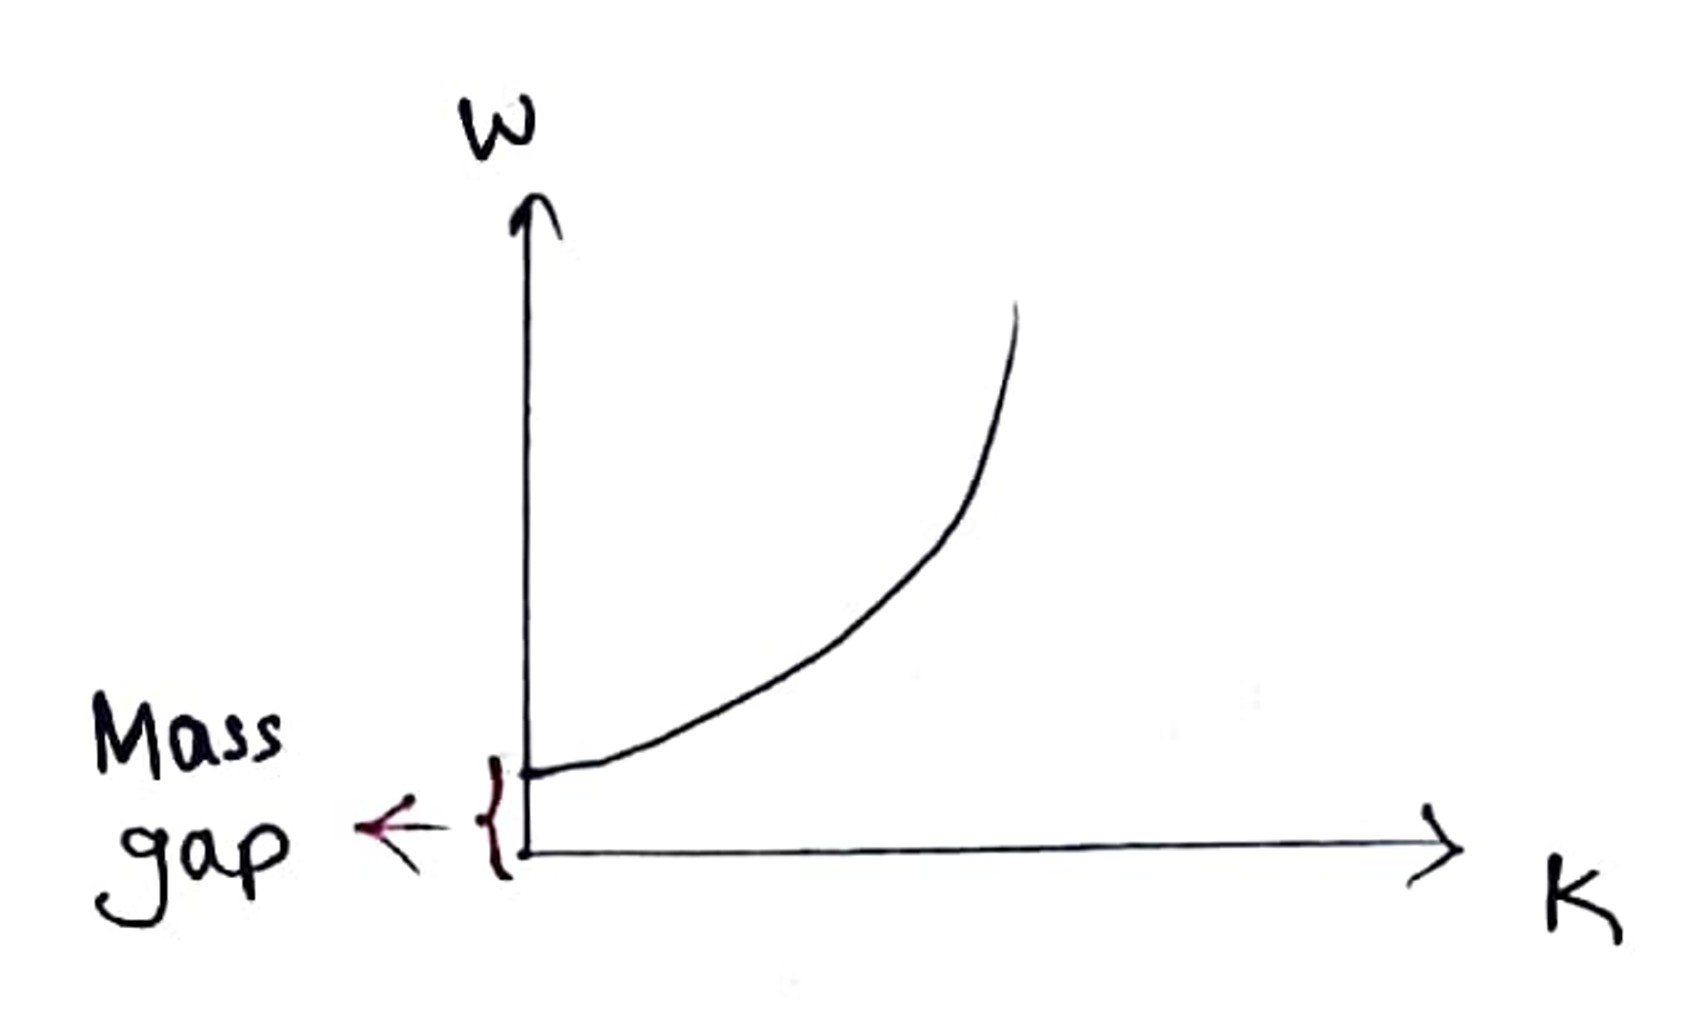
\includegraphics[width=0.6\linewidth]{L(-2)_1.jpg}
\caption*{}
\end{figure}
\vspace{-1.5cm}
\subsection*{Massless}
\begin{itemize}
    \item The relationship is linear.
    \item For photon: $\omega = ck$
    \item True for every relativistic particle.
\end{itemize}
% ---
\begin{figure}[H]
\centering
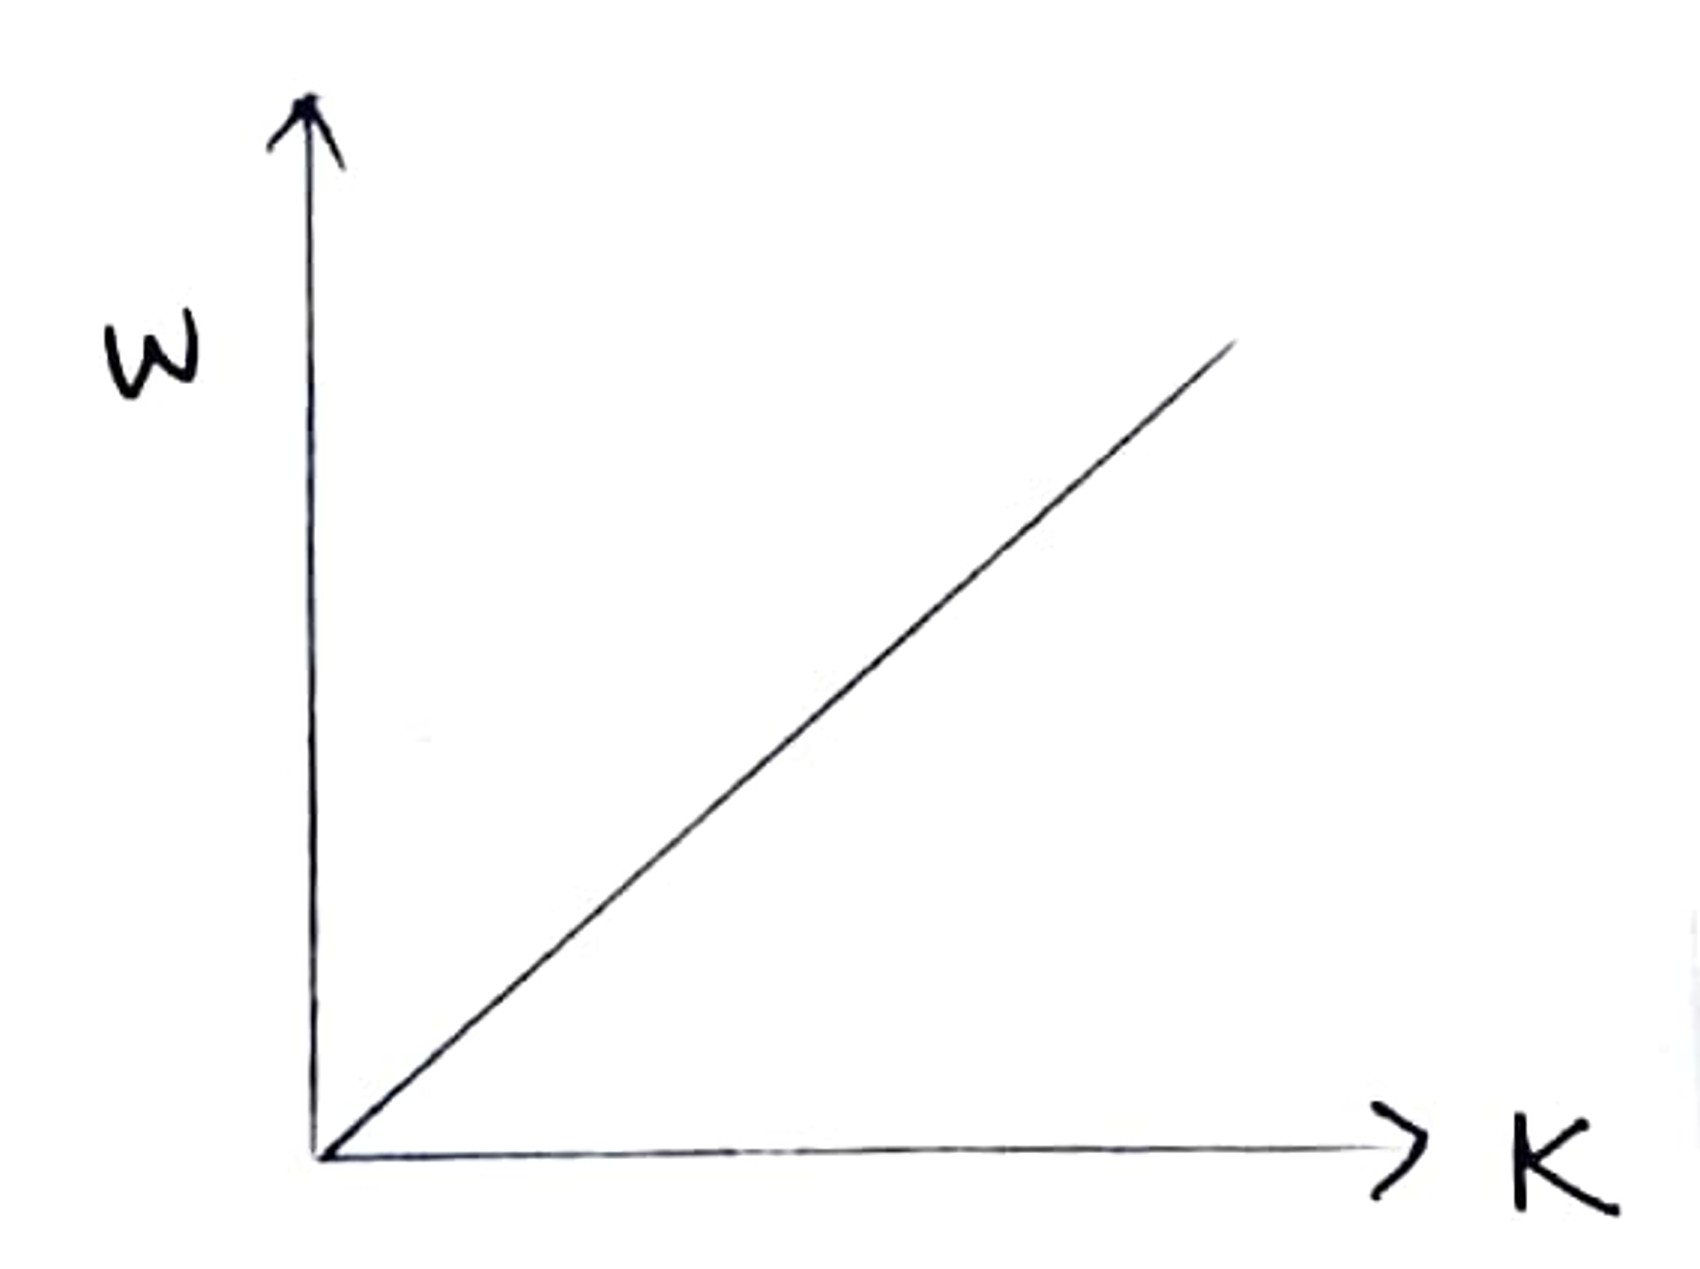
\includegraphics[width=0.45\linewidth]{L(-2)_2.jpg}
\caption*{}
\end{figure}
\vspace{-1cm}
\subsection{Quantum Mechanics}
\textbf{Density matrix} is a more general property than the wave function $\psi$ to represent or describe the state of a quantum system. It arises from an alternative interpretation of the first postulate of quantum mechanics, which asserts that $\psi$ describes the state of a system.
% ---
\subsection*{Fundamental Postulates of Quantum Mechanics:}
\begin{enumerate}
    \item Physical observables are represented by operators. Operators map to real numbers.
    \item States are mathematical objects that assign real expectation values to those operators.
\end{enumerate}
Conditions to be operators:
\[
\omega(\mathbb{I}) = 1 \quad , \quad \omega(A^\dagger A) \geq 0
\]
% ---
\begin{tcolorbox}[ title=\textbf{Question: What is algebra?}]
Algebra is a mathematical structure consisting of a set equipped with one or more operations, where the operations are \textbf{\textit{defined}} and the set is \textbf{\textit{closed}} under those operations.
\end{tcolorbox}
% ---
\textbf{Angular Momentum Operators:}
\begin{itemize}
    \item $[S_1, S_2] = i\hbar\, S_3$ \hfill (finite-dimensional representation)
    \item $[L_1, L_2] = i\hbar\, L_3$ \hfill (infinite-dimensional representation)
\end{itemize}
These are different representations of the same underlying algebraic structures, i.e., representation of a bigger space acting on different vector spaces.
% ---
\subsection*{Probability Interpretation}
\[
\psi \rightarrow \text{Probability Density}
\]
\[
    \int |\psi|^2 \, d\tau = \text{constant} =1
\]
$$\text{Not always right, especially when particle number is not conserved.}$$

This condition is violated when an atom undergoes a decay process, such as:
\[
\text{Atom} \rightarrow \text{Atom} + \bar{\psi}_{\gamma}
\]
\[
    \psi_I \rightarrow \psi_{II} + \bar{\psi}_\gamma
\]
\begin{figure}[H]
\centering
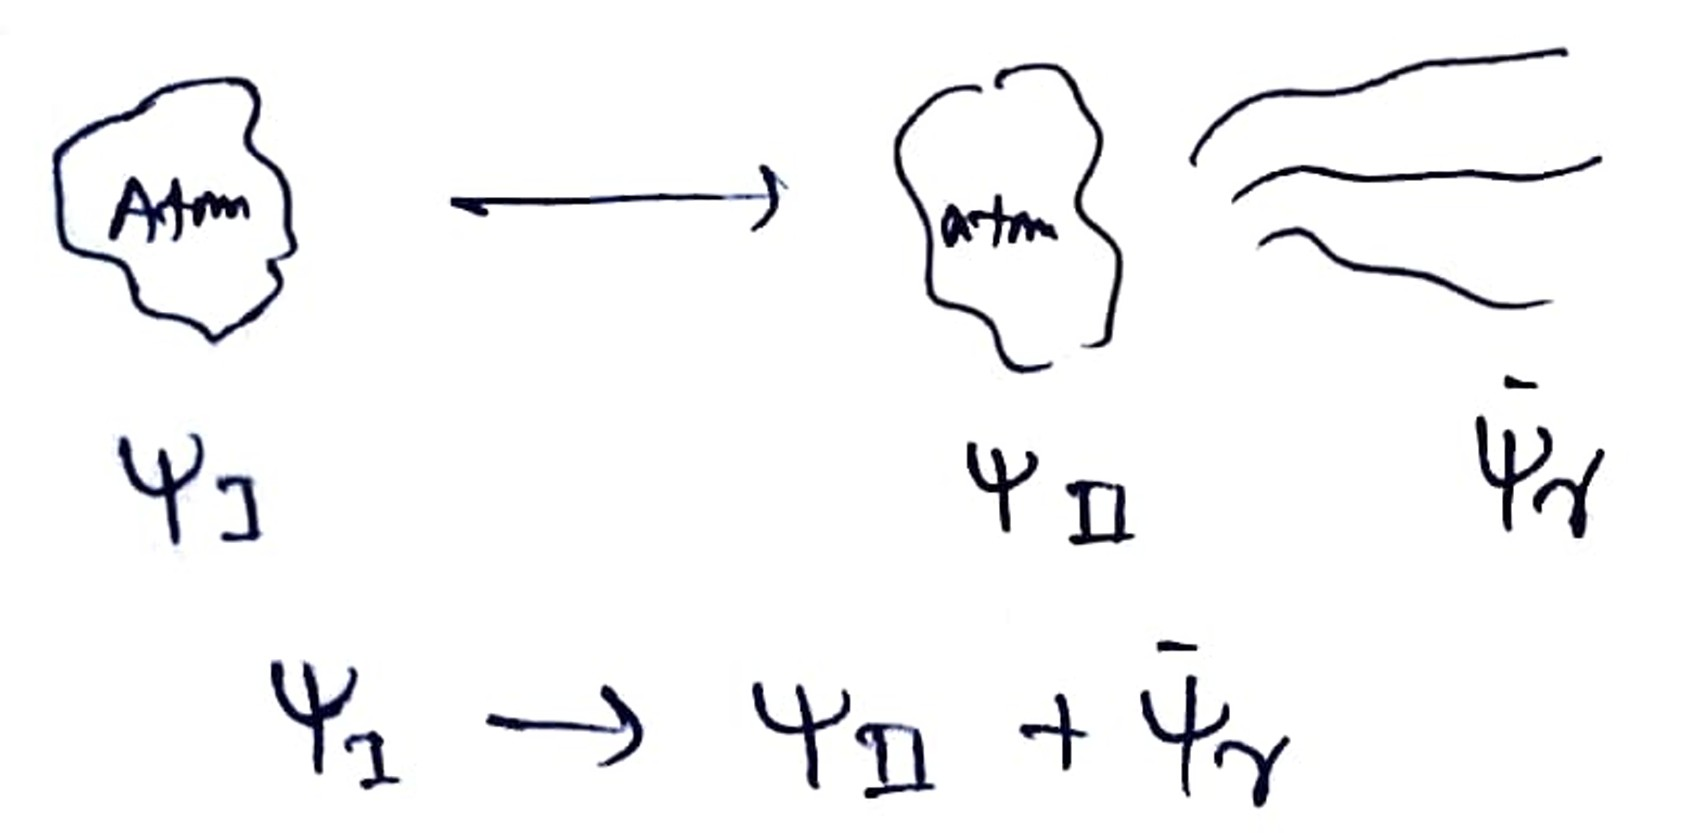
\includegraphics[width=0.6\linewidth]{L(-2)_3.jpg}
\caption*{}
\end{figure}
The conservation of total probability in such transitions implies:
\[
\int |\psi_I|^2 \, d\tau = \int \left(|\psi_{II}|^2 + |\bar{\psi}_\gamma|^2\right) \, d\tau
\]
\subsection*{Two Cornerstones of 20th Century Physics:}
\begin{itemize}
    \item \textbf{Special Relativity:} $E = mc^2$
    \item \textbf{Quantum Mechanics:} $\Delta p \, \Delta x \geq \hbar/2$
\end{itemize}

However, these two principles are not inherently compatible. For instance, taking the uncertainty principle to the limit:
\begin{align*}
    &\Delta x \to 0 ~~\Rightarrow~~ \Delta p~ \to \infty \\
    & \text{As, } \Delta E = \frac{(\Delta p)^2}{2m} \to \infty
\end{align*}
Energy uncertainty generates multi-particles. This leads to new phenomena, such as particle creation, which cannot be fully explained by either theory alone — highlighting the need for \textbf{Quantum Field Theory}. \\
% ---
\textbf{Reading Assignments:}
\begin{tcolorbox}[ title=Reading Assignments:]
\begin{itemize}
    \item Von Neumann — \textit{Mathematical Foundations of Quantum Mechanics}, \\
    (for mathematical formalism and axiomatic treatment.)
    \item Jackson — \textit{Classical Electrodynamics}, Chapters 11 and 12
\end{itemize}
\end{tcolorbox}
\newpage
%-------------------------------
% Section: Lecture 2
%-------------------------------
\stepcounter{section}
\renewcommand{\thesection}{\arabic{section}}
\fancysection{(\textit{\textbf{Class-2})} Lecture \textbf{(-1)}: Sat, Apr 19, 2025}{\textit{Review of Special Relativity}}
% \fancysection{Lecture \textbf{(-1)}: Sat, Apr 19, 2025}{\textit{Review of Special Relativity}}
\begin{itemize}
  \item Collection of events: $\{x\} = \mathcal{M} \rightarrow$ set of events in spacetime
  \item An event can be labelled by 4 coordinates: $x^a,~a = 0,1,2,3$
\end{itemize}
% ---
\subsection{Manifold}
Spacetime is endowed with a manifold structure $\Rightarrow$ means that: spacetime, although it can be curved and complex on a large scale, is treated mathematically as a \textbf{manifold} — a space that, in small patches, looks like regular, flat space and time.
\begin{tcolorbox}[ title=\textbf{Definition}]
A mathematical space on which calculus can be consistently defined. It is typically covered by multiple coordinate charts (or `patches') that together form an ``atlas''.
\[
\text{Spacetime} \rightarrow \text{Manifold } (\mathbb{R}^4)
\]
\end{tcolorbox}
\vspace{-0.5cm}
\begin{figure}[H]
\centering
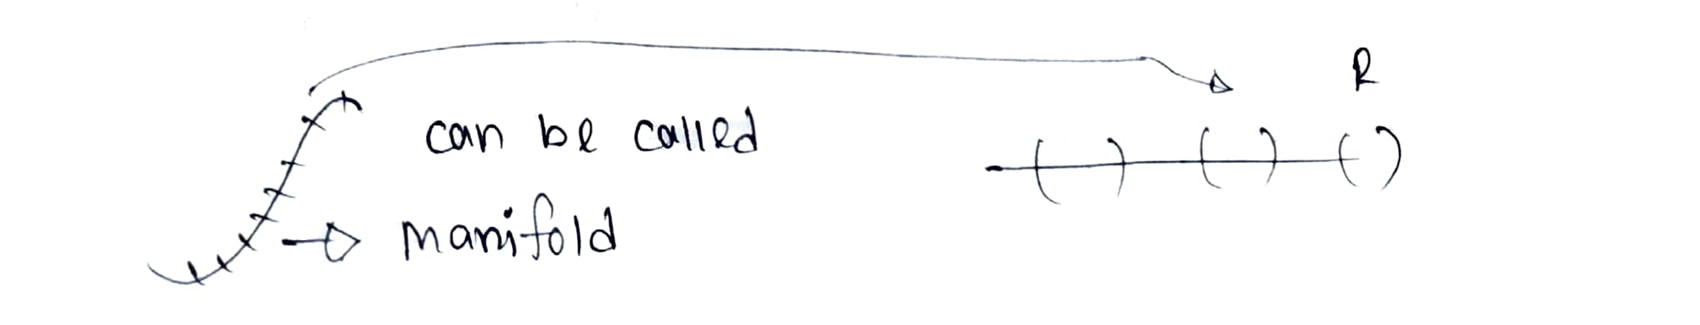
\includegraphics[width=0.9\linewidth]{L(-1)_1.jpg}
\caption*{}
\end{figure}
\vspace{-0.9cm}
\noindent
\underline{Each of the local neighborhood}s in a manifold is \underline{\textit{isomorphic} to line segments} in Euclidean space.
\begin{itemize}
  \item \textbf{Each of the local neighborhoods:} refers to small regions around each point on the manifold.
  \item \textbf{Isomorphic to line segments:} means that they have the same structure, in the sense that we can map one onto the other without losing information.
\end{itemize}
On the other hand,
% ---
\begin{figure}[H]
\centering
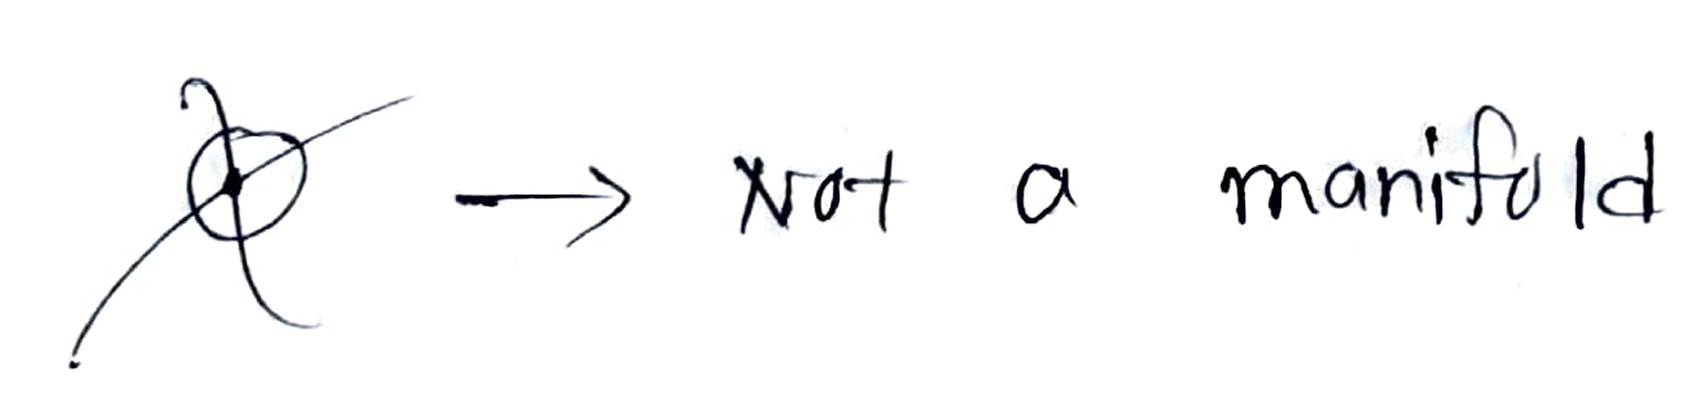
\includegraphics[width=0.5\linewidth]{L(-1)_2.jpg}
\caption*{}
\end{figure}
\vspace{-0.9cm}
\noindent
Because if there are `cuts' in spacetime — like tears, edges or points where the structure breaks down — then spacetime isn't a proper manifold at those points.

\subsection*{Manifold Requirements}
A manifold must satisfy:

\begin{enumerate}
    \item \textbf{Locally Euclidean:} Locally looks like flat space ($\mathbb{R}^4$).
    \item \textbf{Smooth or differentiable:} Calculus can be done.
    \item \textbf{No breaks or cuts:} The space must be continuous and connected in a smooth way.
\end{enumerate}
\noindent
Therefore, when there are `cuts', then at those points, the spacetime fails to be a manifold because smooth coordinates can't be defined or calculus can't be done nicely there.

\subsection*{Difference between SR and GR}
\begin{itemize}
    \item \textbf{SR} needs only one single patch. One single patch can cover everything.
    $$ \text{(A single patch = one coordinate system that works in a specific region of spacetime)} $$
    \item \textbf{GR} needs multiple patches to cover everything.
\end{itemize}

\subsection*{Example: Coordinate Patches on a Sphere}

To describe a sphere (specifically a 2D sphere like the surface of the Earth), at least 2 coordinate patches (charts) are needed to smoothly cover the entire surface.
\begin{center}
    \textbf{A single coordinate system works everywhere except at the poles.}
\end{center}
\begin{figure}[H]
\centering
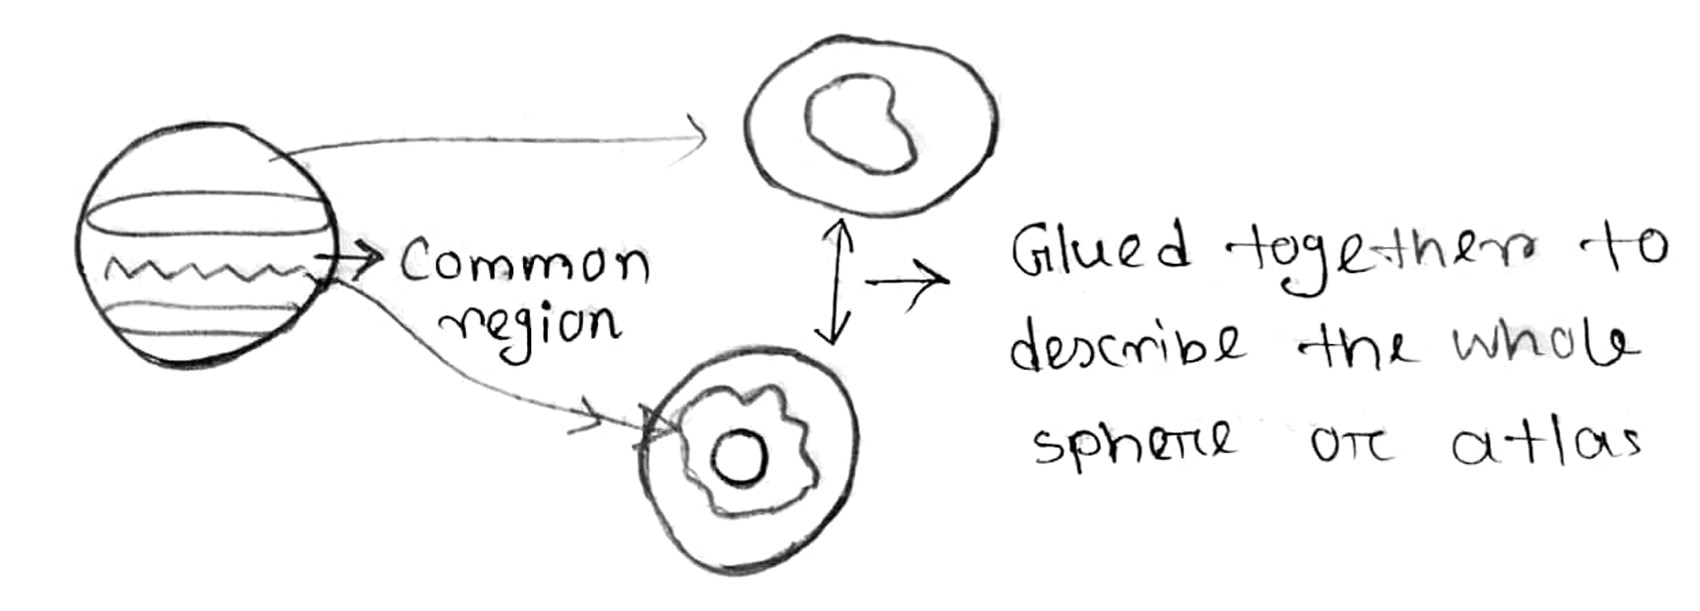
\includegraphics[width=0.8\linewidth]{L(-1)_3.jpg}
\caption*{}
\end{figure}
\vspace{-0.9cm}
\noindent
\textbf{Extra:} 

In $N$ dimensions, we need ${}^NC_2$ angles to describe the coordinate system. \\ \\
\noindent
\textbf{Example:} In 10 dimensions, $ {}^{10}C_2 = 45 $ angles are needed.
\begin{itemize}
    \item $ {}^{10}C_2 $ because we need 2 vectors to define a plane in space.
    \item Rotation is defined in a plane.
\end{itemize}
% ---
\textbf{Now, the spacetime interval (or ``distance-squared") between two events:}
\begin{align*}
    d^2(x, y) &= (x - y)^T H (x - y) \\
    &= (x - y)^a \, \eta_{ab} \, (x - y)^b \\
    &= [(x^0 - y^0)]^2 - (\vec{x} - \vec{y}) \cdot (\vec{x} - \vec{y})
\end{align*}

We use \textbf{East-coast convention:}
\[
H \equiv \eta_{ab} = 
\begin{bmatrix}
1 & 0 & 0 & 0 \\
0 & -1 & 0 & 0 \\
0 & 0 & -1 & 0 \\
0 & 0 & 0 & -1
\end{bmatrix}
\]
In Special Relativity (SR), $\eta$ is fixed and globally defined. However, in General Relativity (GR), the metric becomes a function of position.
\vspace{0.5cm}
$$\fbox{\textbf{\textit{The speed of information transfer is limited by the speed of light.}}}$$
% ---
\begin{figure}[H]
\centering
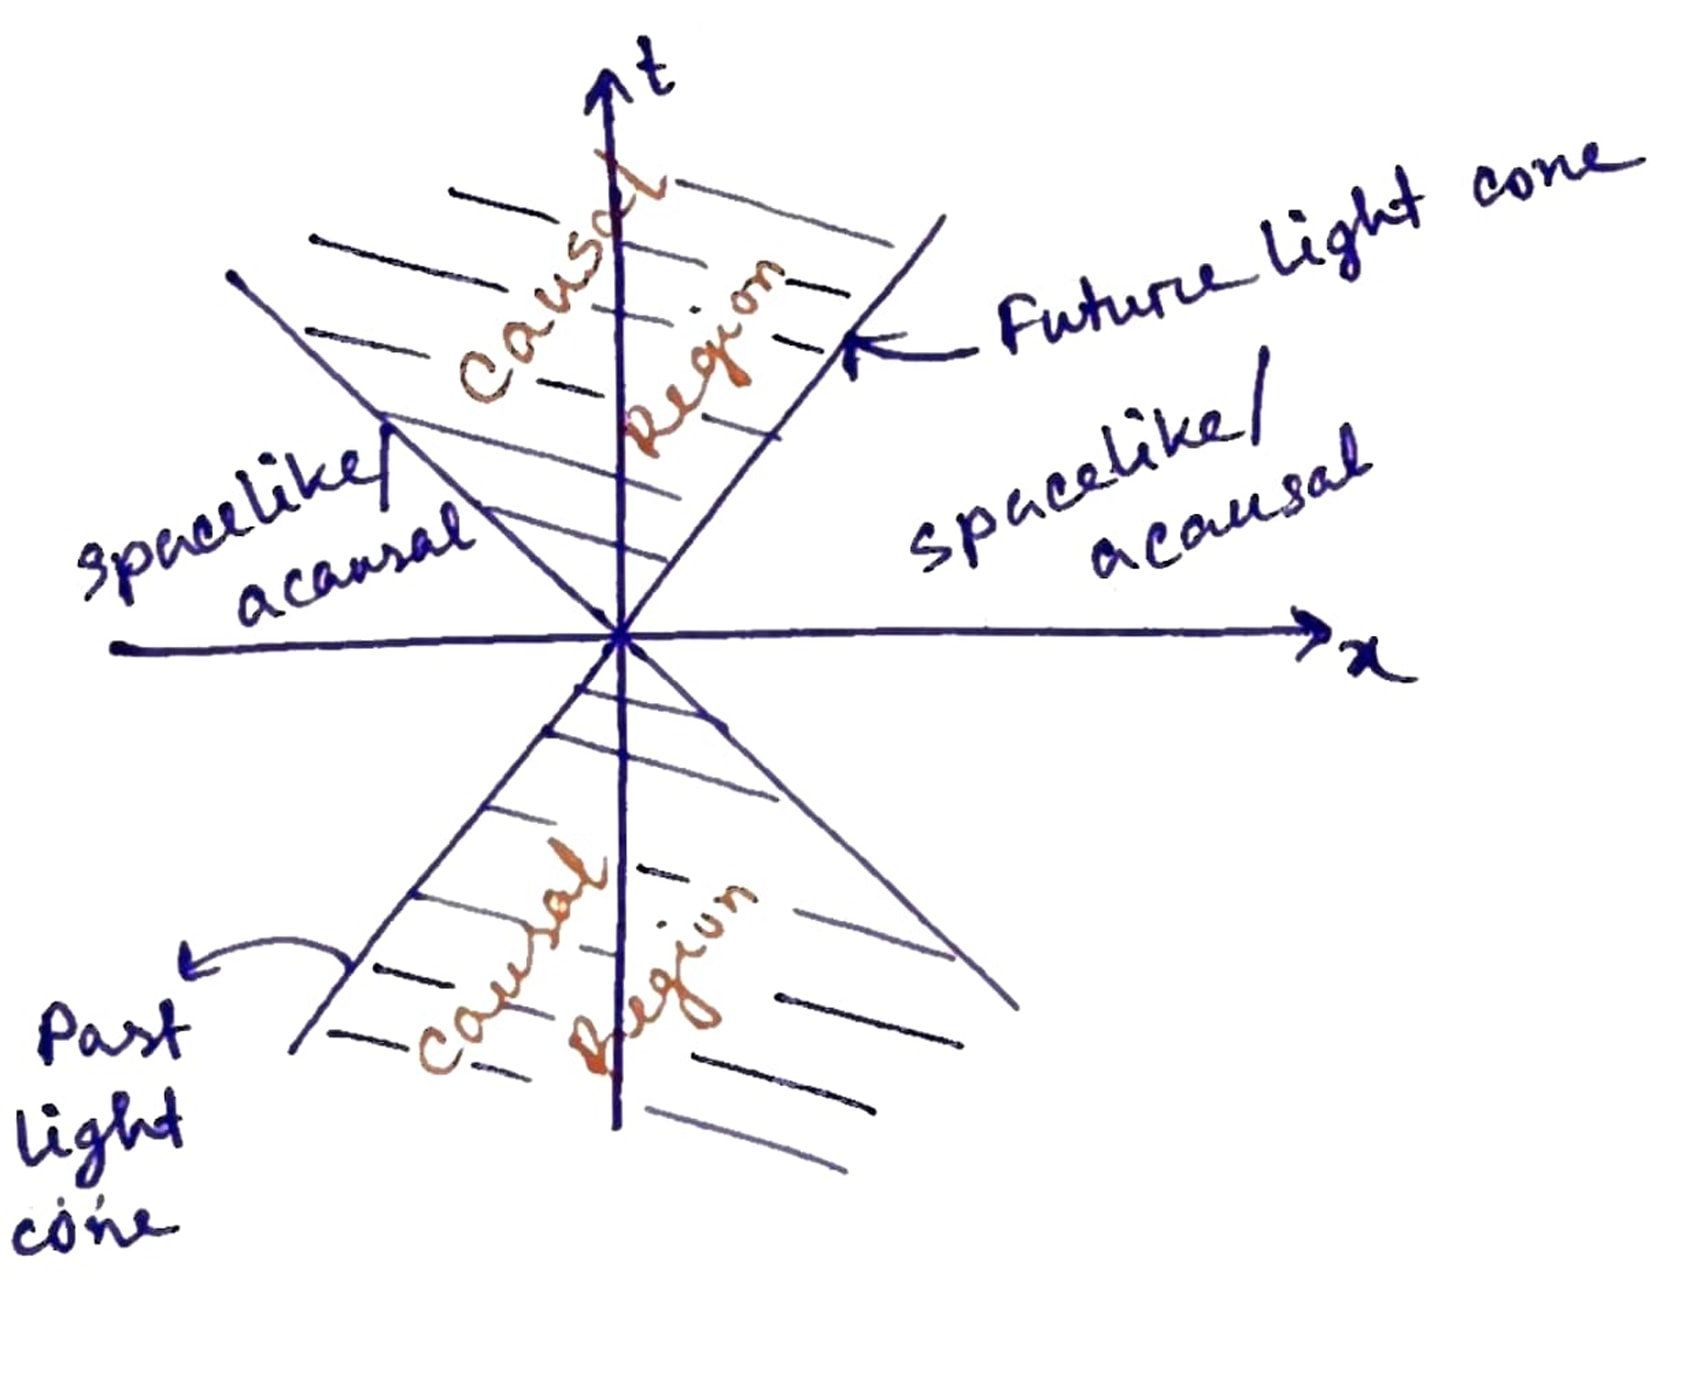
\includegraphics[width=0.6\linewidth]{L(-1)_4.jpg}
\caption*{Figure: Light Cone}
\end{figure}
% \vspace{-1.2cm}
\textbf{Constants and Units:}
\begin{align*}
   & c = 1  \Rightarrow  [L] = [T] \\
   & E = mc^2 \Rightarrow E = m \\
   & \hbar = 1 \Rightarrow ~ \lambda = \frac{\hbar}{mc} \sim \frac{1}{E} \\
   \therefore~ &[M],~[L]~,[T] \equiv E,~ \frac{1}{E},~ \frac{1}{E}
\end{align*}

$$\fbox{\textcolor{red}{\textbf{\textit{By convention, we will measure everything in energy scales.}}}}$$
\vspace{0.3cm}
\begin{tcolorbox}[ title=Postulate 1 :]
Laws of nature must be such that all (\ldots \footnote{Something else wll sit here}) observers\footnote{One who records--- always tied to the coordinate system.} will experience the same causal phenomena.
\end{tcolorbox}
\noindent
This postulate implies that laws must be written using \textbf{tensors} (they are independent of the coordinate system).
\newpage
\subsection*{Galilean Transformations:}
$$ x' = x - vt $$
\begin{itemize}
    \item In frame $S \Rightarrow m \frac{d^2x}{dt^2} = f$
    \item In frame $S' \Rightarrow m \frac{d^2x'}{dt^2} = f'$
\end{itemize}
Under the assumptions: \quad $t' = t, \quad m' = m$ \\
And, since $x' = x - vt$,
\begin{align*}
    f' &= m \dfrac{d^2 x'}{dt'^2} \\
    \Rightarrow f' &= m \dfrac{d^2 (x - vt)}{dt^2} \\
    \Rightarrow f' &= m \dfrac{dv}{dt} \quad [\because\dfrac{d^2}{dt^2}(-vt) = 0] \\
    \Rightarrow f' &= ma \\
    \therefore f'&= f
\end{align*}
$$ \textbf{This invariance is a ``symmetry'' of the Newtonian laws.} $$
% ---
\subsection*{Lorentz Transformations}
Lorentz transformations are linear transformations that keep the ``distance squared'' unchanged.

\[
d^2(x) = x^T H x
\]
\[
x^a \rightarrow x'^a = \Lambda^a_{~b}~x^b \quad [\text{not } \Lambda^a_{b} x^b]
\]
\[
\begin{pmatrix}
x'^0 \\
x'^1 \\
x'^2 \\
x'^3
\end{pmatrix}
=
\begin{pmatrix}
\Lambda^0{}_0 & \Lambda^0{}_1 & \Lambda^0{}_2 & \Lambda^0{}_3 \\
\Lambda^1{}_0 & \Lambda^1{}_1 & \Lambda^1{}_2 & \Lambda^1{}_3 \\
\Lambda^2{}_0 & \Lambda^2{}_1 & \Lambda^2{}_2 & \Lambda^2{}_3 \\
\Lambda^3{}_0 & \Lambda^3{}_1 & \Lambda^3{}_2 & \Lambda^3{}_3
\end{pmatrix}
\begin{pmatrix}
x^0 \\
x^1 \\
x^2 \\
x^3
\end{pmatrix}
\]

\subsection*{Rotations}
\[
\text{If}\quad  x = \begin{pmatrix}
x_1 \\
x_2 \\
x_3
\end{pmatrix}, 
\text{then:} \quad
x^T = \begin{pmatrix}
x_1 & x_2 & x_3
\end{pmatrix}
\]
Hence:
\[
x^T x = 
\begin{pmatrix}
x_1 & x_2 & x_3
\end{pmatrix}
\begin{pmatrix}
x_1 \\
x_2 \\
x_3
\end{pmatrix}
= x_1^2 + x_2^2 + x_3^2
= r^2
\]
Now, under rotation:
\[
x \to x' = R x
\]
Then,
\begin{align*}
    (x')^T x' &= (Rx)^T (Rx) \\
    &= x^T R^T R x \\
    &= x^T x
\end{align*}
Therefore:
\[
\therefore\boxed{  R^T R = R^T \mathbb{I} R = \mathbb{I}}
\]
Similarly, under Lorentz transformation:
\begin{align*}
    d^2(x') &= x'^T H x' \\
    &= (\Lambda x)^T H (\Lambda x) \\
    &= x^T~\Lambda^T H \Lambda~x \\
    &= x^T H x
\end{align*}
\[
\therefore \boxed{\Lambda^T H \Lambda = H}
\]
Just as $R^T R = \mathbb{I}$ defines orthogonal transformations, $\Lambda^T H \Lambda = H$ defines Lorentz transformations.
$$\fbox{$\left[R^T R = I\right] \subset \left[\Lambda^T H \Lambda = H\right]$ \text{are the examples of classical groups.}}$$

\subsection*{Dynamics}
\begin{figure}[H]
\centering
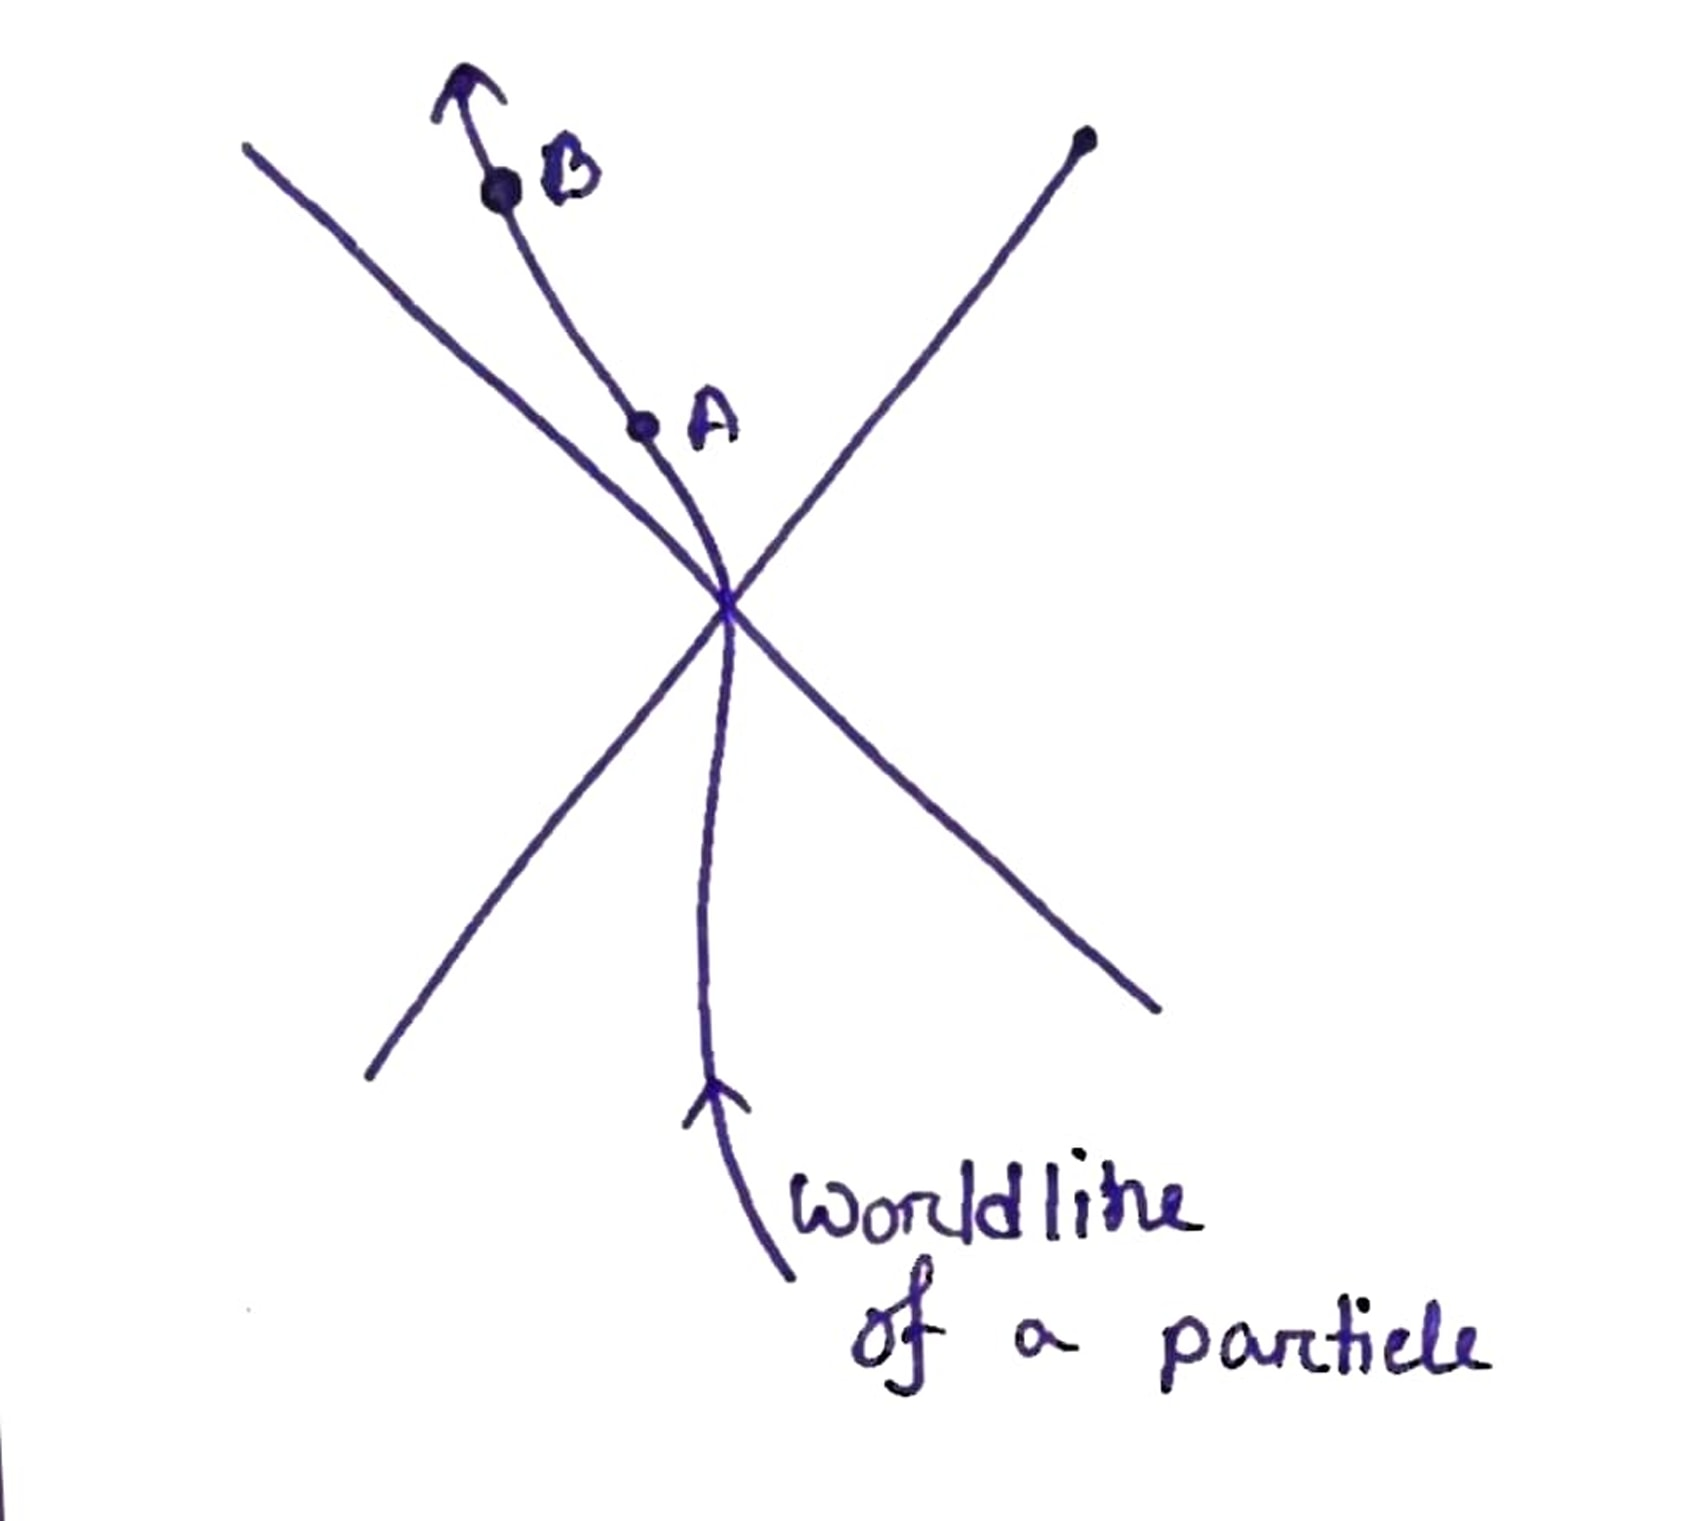
\includegraphics[width=0.5\linewidth]{L(-1)_5.jpg}
\caption*{}
\end{figure}
\vspace{-1cm}
\begin{itemize}
    \item Let $A \to x = (x^0, x^1, x^2, x^3)$
    \item $B \to x + dx = (x^0 + dx^0, \ldots, x^3 + dx^3)$
\end{itemize}
Hence,
\[
d^2(A,B) = (dx^0)^2 - d\vec{x} \cdot d\vec{x} = d\tau^2
\]

For a comoving observer, we have $$d\vec{x} = 0$$
\[
\text{thus:}~ d\tau^2 = (dx^0)^2
\]
\[
\textbf{(Time dilation simply arises from this equation)}
\]
\begin{itemize}
    \item If $d^2(A,B) \to$ constant (let it be 10), then:
    $$d\tau^2 \to 10 \quad \text{(comoving)} \quad [\because d\vec{x} \cdot d\vec{x} = 0] $$
    
    \item If not comoving, say $d\vec{x} \cdot d\vec{x} = 3$, then to keep $d^2(A,B) = 10$, we need to have:
     $$(dt)^2 = d^2(A,B) + d\vec{x} \cdot d\vec{x} = 10 + 3 = 13$$ 
    $$\text{Thus,}~ \boxed{(dt)^2 \neq (d\tau)^2 }$$
\end{itemize}
% ===
\subsection*{Proper Time ($\tau$)}
\begin{align*}
    \tau &= \text{Time measured by an observer moving along the worldline} \\
    &= \text{Time measured by a co-moving observer}
\end{align*}
\begin{align*}
    d\tau^2 &= dt^2 - d\vec{x} \cdot d\vec{x} \\
    \Rightarrow 1 &= \left( \frac{dt}{d\tau} \right)^2 - \left( \frac{d\vec{x}}{d\tau} \right)^2 \\
   &\left[\text{here, } u^a = \left( \frac{dt}{d\tau}, \frac{d\vec{x}}{d\tau} \right)\right] \\
    \Rightarrow u^a u_a &= u \cdot u = 1
\end{align*}
As we know,
\[
\boxed{u \cdot u 
\begin{cases}
>0 & ;\quad  \text{Timelike} \\
<0 & ;\quad \text{Spacelike} \\
=0 & ;\quad \text{Lightlike}
\end{cases}}
\]
Then:
\[
u \cdot u = 1 \quad \therefore \textbf{4-velocity is timelike}
\]
\vspace{-1cm}
\subsection*{Significance}
\begin{enumerate}
    \item The worldline of a massive object always stays inside the light cone --- it can never go faster than light.
    \item The object is always moving forward in time according to its own clock.
    \item If it were spacelike, that would imply faster-than-light motion.
\end{enumerate}
\begin{align*}
    \text{Now, }u \cdot u &= 1 \\
    \Rightarrow \frac{du^a}{dt} u_a &+ \frac{du_a}{dt} u^a = 0 \\
    \Rightarrow \frac{du^a}{dt} &u_a = 0 \\
    \Rightarrow a^b u_b &= 0
\end{align*}
\begin{figure}[H]
\centering
\begin{minipage}[c]{0.45\textwidth}
\[
\Rightarrow \text{4-acceleration} \perp \text{4-velocity}
\]
\[
\therefore \textbf{4-acceleration is spacelike}
\]
\end{minipage}
\hfill
\begin{minipage}[c]{0.5\textwidth}
\centering
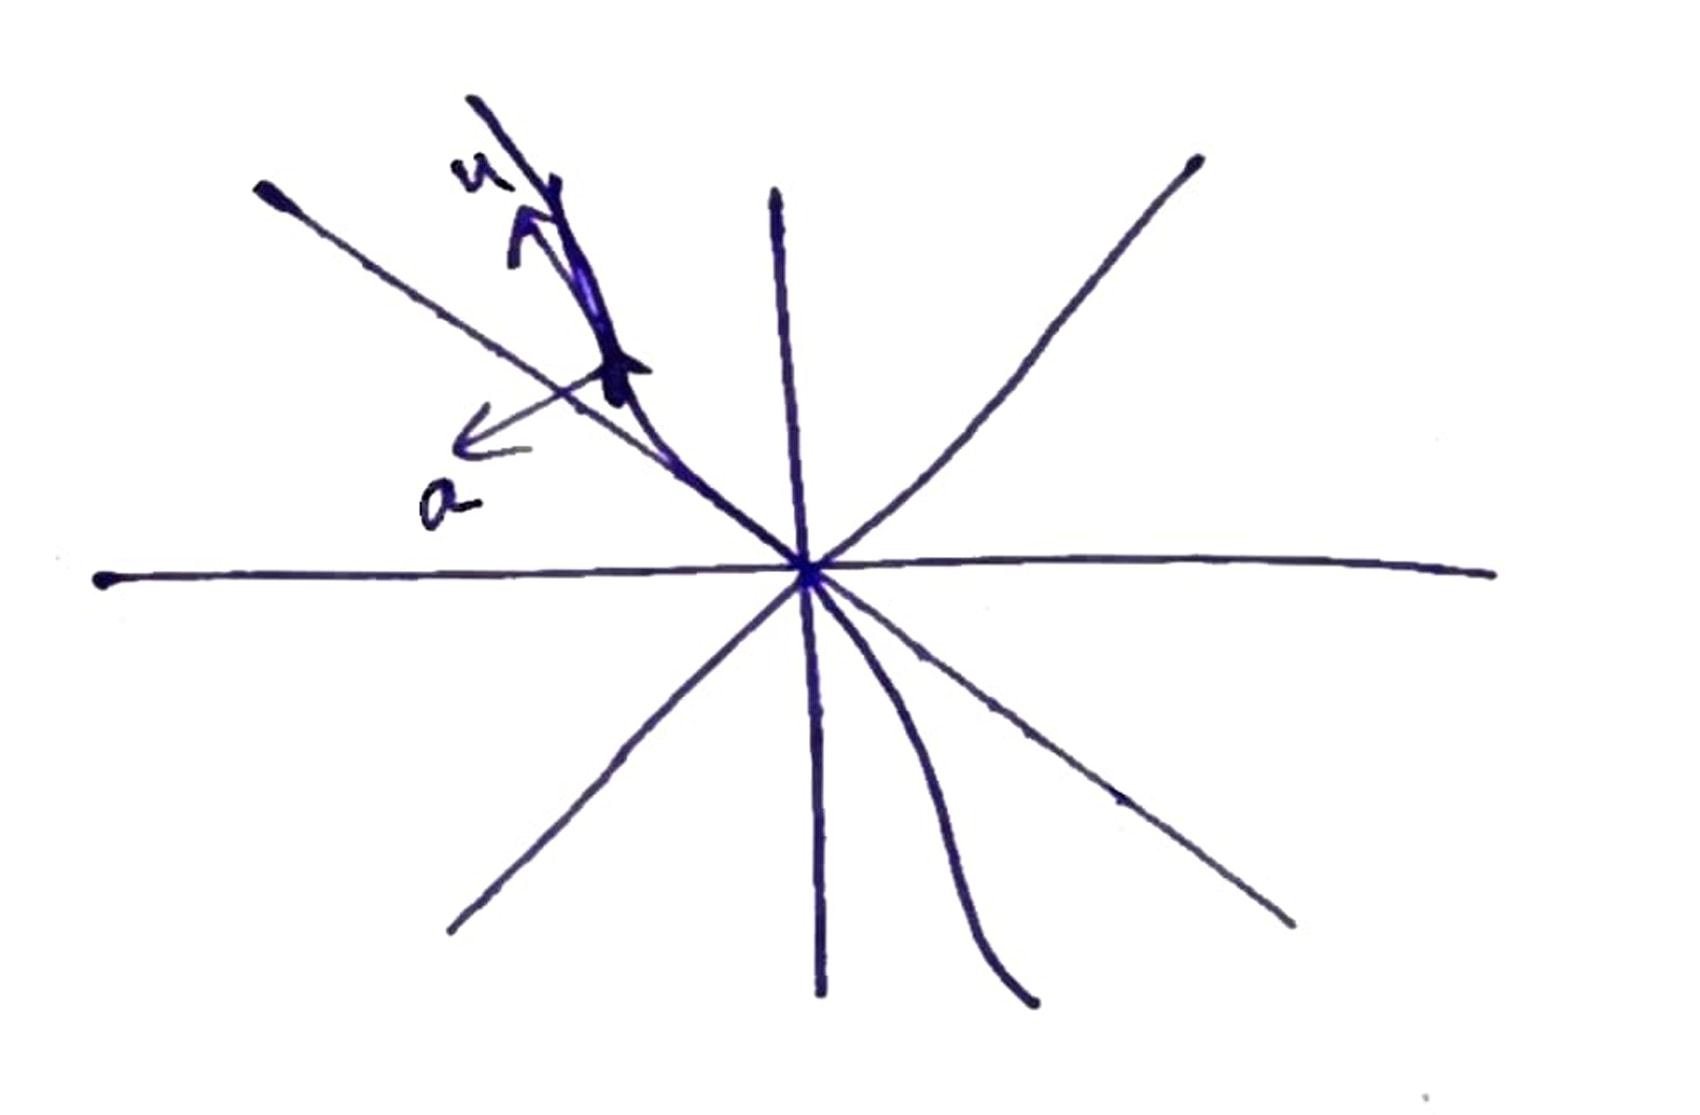
\includegraphics[width=\linewidth]{L(-1)_6.jpg}
\end{minipage}
\end{figure}
% ---
\newpage
\textbf{Significance:}
\begin{enumerate}
    \item It is not contributing to your time flow.
    \item It changes spatial direction through spacetime.
    \item The 4-acceleration only bends the path, it doesn't speed up or slow down in the time direction.
\end{enumerate}
% ---
\subsection*{Lorentz Force}

Relativistic generalization of Newton's second law:
\[
f^b = m a^b \quad \text{(Four-force)}
\]

In an electromagnetic field:
\begin{align*}
    &\quad~~~ a^b = F^b_{\ c} u^c \\
   &\Rightarrow a_b = F_{bc} u^c \quad \quad\quad [\text{Lowering the index}] \\
   &\Rightarrow a_b u^b = F_{bc} u^b u^c \quad~[\text{Contracting with}~u^b] \\
   &\Rightarrow F_{bc} u^b u^c = 0 \quad~~\quad[\text{Since }a^b u_b = 0] \\  
   &\Rightarrow F_{bc} u^b u^c + F_{bc} u^b u^c = 0 \\
   &\Rightarrow F_{bc} u^b u^c + F_{cb} u^c u^b = 0 \\
   &\Rightarrow F_{bc} u^b u^c + F_{cb} u^b u^c = 0 \quad\{\because [u^b,u^c]=0 \}\\
    &\Rightarrow \left(F_{bc} + F_{cb}\right) u^b u^c = 0 \\
    &\therefore F_{bc} = -F_{cb}  
\end{align*}
$$\fbox{
\textbf{\textit{The field strength tensor is antisymmetric.}}
}
$$
The classical (3-vector) form of the Lorentz force law:
\[
m \vec{a} = q \left( \vec{E} + \vec{v} \times \vec{B} \right)
\]

Relativistic form:
\[
m \frac{du^a}{d\tau} = q F^a_{\ b} u^b
\]

Field strength tensor $F^{ab}$:
\[
F^{ab} \equiv
\begin{bmatrix}
0 & -E_x & -E_y & -E_z \\
E_x & 0 & -B_z & B_y \\
E_y & B_z & 0 & -B_x \\
E_z & -B_y & B_x & 0
\end{bmatrix}
\]
% ---
\subsection*{Action Principle}
$$ \text{Action,}~ S \Rightarrow \delta S = 0 \quad \text{[minimum]} $$
$$ \textbf{(Observer independent)} $$
\[
\Downarrow \quad \text{consequence}
\]
$$\text{Euler-Lagrange (EL) equations.}$$
$$ \textbf{The action should be invariant under coordinate transformation.} $$
\begin{align*}
    S &\propto \text{proper length of worldline} \\
    \Rightarrow S &\propto \int d\tau \\
    \Rightarrow S &= m \int d\tau
\end{align*}
$$ \text{(where m is not relativistic mass, no relativistic mass exists.)} $$
$$\textbf{Action must be scalar, no change will happen under transformation.}$$
\\
\textbf{Dimensional Analysis of Action:}
\begin{itemize}
    \item $S$ is dimensionless
    \item $d\tau$ has units of length
    \item $m$ has units of inverse length
\end{itemize}
\begin{align*}
    S[x] &= m \int \sqrt{ \eta_{ab} \, dx^a dx^b }=m \int d \tau \\
    &= m \int \sqrt{ \eta_{ab} \, \frac{dx^a}{d\lambda} \frac{dx^b}{d\lambda} } \, d\lambda 
\rightarrow \text{(Reparameterization invariant)}
\end{align*}
$$(d\lambda\text{ can be any time, not necessarily just proper time})$$
\noindent
\textbf{HW:} \quad Derive the Euler–Lagrange equations corresponding to this action (Note: The Hamiltonian of this system is zero.)
% --- HW ---
\begin{framed}
\vspace{-0.5cm}
\subsection*{Solving the HW problem:}
Given, the action
\[
A[x(s)] = m \int_{s_1}^{s_2} \sqrt{\eta_{ab} \frac{dx^a}{ds} \frac{dx^b}{ds}} \, ds
\]
Where the Lagrangian:
\[
\mathcal{L}(\dot{x}^a, \dot{x}^b) = m\left( \eta_{ab}~\dot{x}^a\dot{x}^b \right)^{1/2}
\]
\noindent
Now, consider a variation in $x(s)$:
\[
x(s,\epsilon) = x(s,0) + \epsilon\eta(s)
\]
with the boundary condition:
\[
\eta(s_1) = \eta(s_2) = 0 \quad \text{[end points]}
\]
Therefore, the variation in the action is:
\begin{align*}
\delta A &= \delta \int_{s_1}^{s_2} \mathcal{L} \left( \dot{x}^a\left( s \right), \dot{x}^b \left(s\right) \right) ds \\
\Rightarrow \delta A &= m \int_{s_1}^{s_2} \left( \frac{\partial \mathcal{L}}{\partial \dot{x}^a}~ \frac{\partial \dot{x}^a}{\partial \epsilon} d\epsilon + \frac{\partial \mathcal{L}}{\partial \dot{x}^b}~\frac{\partial \dot{x}^b}{\partial \epsilon} d\epsilon \right) ds \\
\\
\Rightarrow \delta A &= m \int_{s_1}^{s_2} \left[ 
\frac{\dot{x}^a}{\sqrt{\dot{x}^b~ \dot{x}_b}}~ \frac{\partial^2 {x}^a}{\partial \epsilon~\partial s}~d \epsilon 
+ 
\frac{\dot{x}^b}{\sqrt{\dot{x}^a~\dot{x}_a}}~ \frac{\partial^2{x}^b}{\partial \epsilon~\partial s}~d\epsilon 
\right] ds \\
\\
\Rightarrow \delta A &= m \int_{s_1}^{s_2} \left[ 
\frac{\dot{x}^a}{\sqrt{\dot{x}^b~\dot{x}_b}} \frac{\partial^2{x}^a}{\partial \epsilon \partial s} d \epsilon 
+ 
\frac{\dot{x}^b}{\sqrt{\dot{x}^a~\dot{x}_a}} \frac{\partial^2 {x}^b}{\partial \epsilon \partial s} d \epsilon
\right] ds \\
\\
&\text{Now using integration by parts:} \\
% -----
\delta A &= m
\left\{ 
\left[ 
\frac{\dot{x}^a}{\sqrt{\dot{x}^b \dot{x}_b}} \frac{\partial x^a}{\partial \epsilon} \Bigg|_{s_1}^{s_2}
- \int_{s_1}^{s_2} \frac{d}{ds} \left( \frac{\dot{x}^a}{\sqrt{\dot{x}^b \dot{x}_b}} \right) \frac{\partial x^a}{\partial \epsilon} \, d \epsilon
\right] \right. \\
&\quad + \left. \left[ 
\frac{\dot{x}^b}{\sqrt{\dot{x}^a \dot{x}_a}} \frac{\partial x^b}{\partial \epsilon} \Bigg|_{s_1}^{s_2}
- \int_{s_1}^{s_2} \frac{d}{ds} \left( \frac{\dot{x}^b}{\sqrt{\dot{x}^a \dot{x}_a}} \right) \frac{\partial x^b}{\partial \epsilon} \, d \epsilon
\right]
\right\} ds
\\
&\text{Since } \eta(s_1) = \eta(s_2) = 0,\ \text{boundary terms vanish:} \\
\\
\delta A &= m \left[ 
- \int_{s_1}^{s_2} \frac{d}{ds} \left( \frac{\dot{x}^a}{\sqrt{\dot{x}^b~\dot{x}_b}} \right) \frac{\partial x^a}{\partial \epsilon} d\epsilon 
- \int_{s_1}^{s_2} \frac{d}{ds} \left( \frac{\dot{x}^b}{\sqrt{\dot{x}^a~\dot{x}_a}} \right) \frac{\partial x^b}{\partial \epsilon} d\epsilon 
\right] ds \\
\text{ If a = b then , } \\
\delta A &= m \left[ 
-2 \int_{s_1}^{s_2} \frac{d}{ds} \left( 
\frac{\dot{x}_a}{\sqrt{\dot{x}^b~\dot{x}_b}} 
\right)\right] \frac{\partial x^a}{\partial \epsilon} d\epsilon  ds  
\end{align*}
if a $\neq$ b , two integrands are separately zero.
Therefore, for the action to be minimum i.e. to be zero, the integrands must be zero.
Hence, we get the Euler-Lagrange equation:
\[
\boxed{m \frac{d}{ds} \left( \frac{\dot{x}_a}{\sqrt{\dot{x}^b~\dot{x}_b}} \right) = 0}
\]
\end{framed}
\newpage
%-------------------------------
% Section: Lecture 0
%-------------------------------
\stepcounter{section}
\renewcommand{\thesection}{\arabic{section}}
\fancysection{(\textit{\textbf{Class-3})} Lecture \textbf{0}: Thrs, Apr 24, 2025}{\textbf{\textit{Preliminary QFT}}}
\subsection{Action for a Point Particle (Massive)}
The action is given by
\begin{equation}
    S = m \int d\tau \tag{1} \label{eq:1}
\end{equation}
where $d\tau$ can be anything, just with respect to a comoving observer.

Expanding,\\
% ---
\begin{minipage}[c]{0.5\textwidth}
\begin{align*}
    S &= m \int \sqrt{\eta_{ab} \, dx^a \, dx^b} \\
      &= m \int \sqrt{\eta_{ab} \frac{dx^a}{d\lambda} \frac{dx^b}{d\lambda}} d\lambda \\
      &= ~~\int \mathcal{L}(x, \dot{x}) \, d\lambda \tag{2} \label{eq:2}
\end{align*}
\end{minipage}
\hfill
\begin{minipage}[c]{0.45\textwidth}
\begin{align*}
    \text{where,}\quad \lambda & : \quad \text{personal time (subjective)} \\
    \tau & : \quad \text{objective time}
\end{align*}
\end{minipage}
% ---
Now, 
\[
\int_a^b dy = y(b) - y(a)
\]
represents coordinates $dy$ can also be written as $$dy = \frac{df}{dy} \, dy$$
Therefore it is geometrical in nature and hence reparameterization invariant.

From equation \eqref{eq:2}, the conjugate momenta will be -
\begin{align*}
    p_a &= \frac{\partial \mathcal{L}}{\partial \dot{x}^a} \tag{3} \label{eq:3} \\
    \Rightarrow p_a &= \frac{\partial}{\partial \dot{x}^a} \left[ m \sqrt{\eta_{ab} ~\dot{x}^a \dot{x}^b} \right] \\
    \Rightarrow p_a &= m\frac{\left( \eta_{ab}~ \dot{x}^b + \eta_{ab}~ \dot{x}^a~ \delta^b_{~a} \right)}{2 \sqrt{\dot{x}^b \dot{x}_b}} \\
    [&\because \frac{\partial \dot{x}^b}{\partial \dot{x}^a} = \delta^b_{~a}] \\
     \Rightarrow p_a &= m\frac{\left(\dot{x}_a + \dot{x}_a\right)}{2 \sqrt{\dot{x}^b \dot{x}_b}} \\
    \therefore p_a &= \frac{m\dot{x}_a}{\sqrt{\dot{x}^b \dot{x}_b}} \tag{4} \label{eq:4}
\end{align*}
\begin{tcolorbox}[ title=\textbf{Note: How are $p$ and $v$ related?}]
The trivial answer is $p = mv$, but more generally,
\[
p_a = \frac{\partial \mathcal{L}}{\partial \dot{x}^a}.
\]
Here, $p_a$ is the cotangent vector, i.e., the dual of the tangent vector ($\dot{x}^a$).
\end{tcolorbox}
Now, the Hamiltonian is:
\begin{align*}
    H &= p_a \dot{x}^a - \mathcal{L} \\
      &= \frac{m\dot{x}_a}{\sqrt{\dot{x}^b \dot{x}_b}} \dot{x}^a - m \sqrt{\dot{x}_c \dot{x}^c} \\
      &= \frac{mr^2}{\sqrt{r^2}} - m \sqrt{r^2} \quad [\because \dot{x}_a \dot{x}^a=r^2]\\
      &= m\sqrt{r^2} - m \sqrt{r^2} \\
      &= 0
\end{align*}
\subsection*{Significance:}
As the Hamiltonian is the generator of time, and for this system it is zero implies that the worldline is fixed. The history of the particle (i.e., the trajectory) is known. There is no evolution of the system, no dynamics of the system. Only spacetime exists. Dynamics is the construction of spacetime itself in our head.

\subsection*{Equation of Motion and Phase Space}
The hallmark difference between Hamilton's and Lagrangian's equations of motion is that Hamilton's equations are first order in time, whereas those of Lagrange's are second order in time.

Example:

\begin{enumerate}
    \item 
\[
    \frac{d\vec{S}}{d\tau} = \mu \, \vec{S} \times \vec{B}
    \longrightarrow \text{Hamilton's equation of motion,} \textbf{ first order in time.}
\]
    
    And the Hamiltonian is:
\[
    H = \frac{1}{2\mu} S_a S^a
\]
    
    Here, $\{s\} \rightarrow$ The set of all spin components constitute the phase space. In the cross-product, there are 3 components and so, the phase space is 3-dimensional.

    \item 
    Similarly, the phase space constituted by $x$ and $p$ is 2-dimensional because
\[
    \frac{dx}{dt} = \{x, H\}_{\text{PB}} \quad \text{and} \quad \frac{dp}{dt} = \{p, H\}_{\text{PB}}
\]

    \item 
    Also, in the Heisenberg picture,
\[
    \frac{dA}{dt} = \frac{1}{i\hbar} [H, A] \quad \text{(three such equations)}
\]
\end{enumerate}
\subsection*{Fun Fact: Relativity of Simultaneity}
It is the concept that distant simultaneity—whether two spatially separated events occur at the same time—is not absolute but depends on the observer's reference frame.
% ---
\begin{figure}[H]
\centering
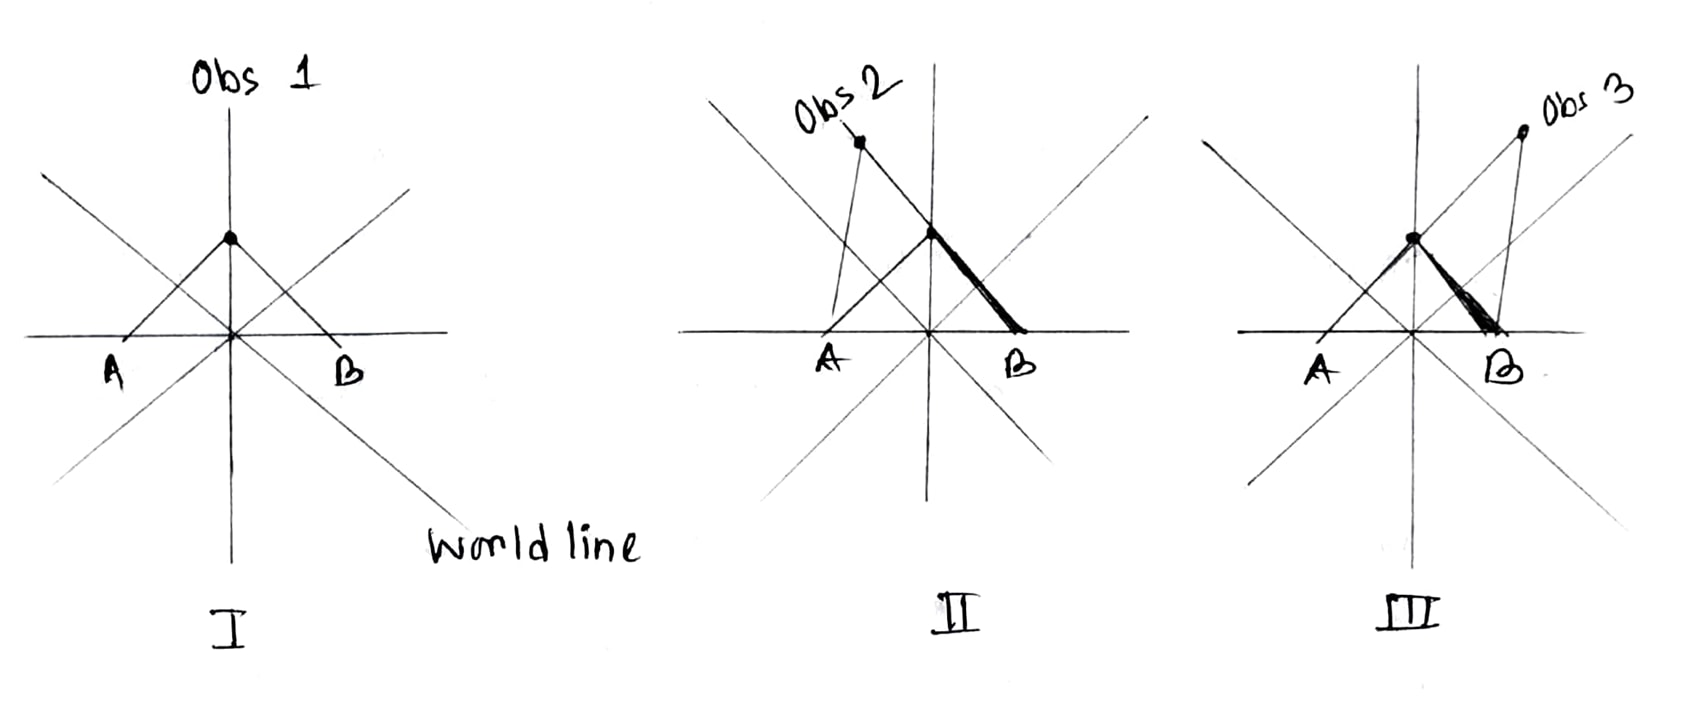
\includegraphics[width=0.9\linewidth]{L0_1 (1).jpg}
\caption*{}
\end{figure}
\vspace{-1.5cm}
\begin{itemize}
    \item The physical laws are always observer independent.
    \item But the order of events, i.e., the \textbf{history} is observer dependent
    \item In picture-I: For observer 1, both events A and B happen simultaneously.
    \item In picture-II: A happens first, then B.
    \item In picture-III: B happens first, then A.
\end{itemize}
$$ \boxed{\therefore \textbf{Simultaneity is not a covariant statement.}} $$
\subsection*{Back to the point particle}
As we know,
\[
p_a = \frac{\partial \mathcal{L}}{\partial \dot{x}^a} = \frac{m \dot{x}_a}{\sqrt{\dot{x}^b \dot{x}_b}}
\]
It might seem that, as in $\dot{x}^a$ there are 4 components, so will be $p_a$. But it's not. The system may seem unconstrained, but it's not!
\[
p^a p_a = \frac{m \dot{x}^a}{\sqrt{\dot{x}^b \dot{x}_b}} \times \frac{m \dot{x}_a}{\sqrt{\dot{x}^b \dot{x}_b}} = \frac{m^2 \dot{x}^a \dot{x}_a}{(\dot{x}^b \dot{x}_b)} = \frac{m^2r^2}{(\sqrt{r^2})^2} = m^2
\]
Thus,
\[
p^a p_a = m^2
\]
\[
\therefore p^2 = m^2 \tag{5} \label{eq:5}
\]
\subsection*{How to quantize a system:}
In an unconstrained (and Cartesian) system,
\[
p_i \leftrightarrow -i ~\partial_i, \quad [\hbar = 1] \quad \text{(In Schrödinger picture)}
\]
This is intimately connected to the coordinate system and works only in Cartesian. Moreover, this correspondence is not unique: Adding $G(x)$ doesn't change the system, as $[\hat{x}_i, \hat{p}_j] = i$ still works.

So, to satisfy $[\hat{x}_i, \hat{p}_j] = i$, it's a realization that
\[
p_i \to -i \partial_i
\]
\begin{framed}
\noindent
\textbf{Dirac's quantization procedure for constrained systems}
%\textbf{Dirac Method:}
\begin{enumerate}
\item Start with classical system, with constraints, e.g., $\phi(q, p) = 0$.
\item Promote variables to operators: $q \to \hat{q}$, $p \to \hat{p}$.
\item Promote constraints too: \quad $\phi(q,p) \rightarrow \hat{\phi}(\hat{q}, \hat{p})$
\item Impose constraints on states: $$\hat{\phi} \ket{\psi} = 0$$
\end{enumerate}
This will tell which quantum systems are physical.
\end{framed}
\noindent
\textbf{Example 1: Particle on a Circle}\\
\vspace{-0.7cm}
\begin{figure}[H]
\centering
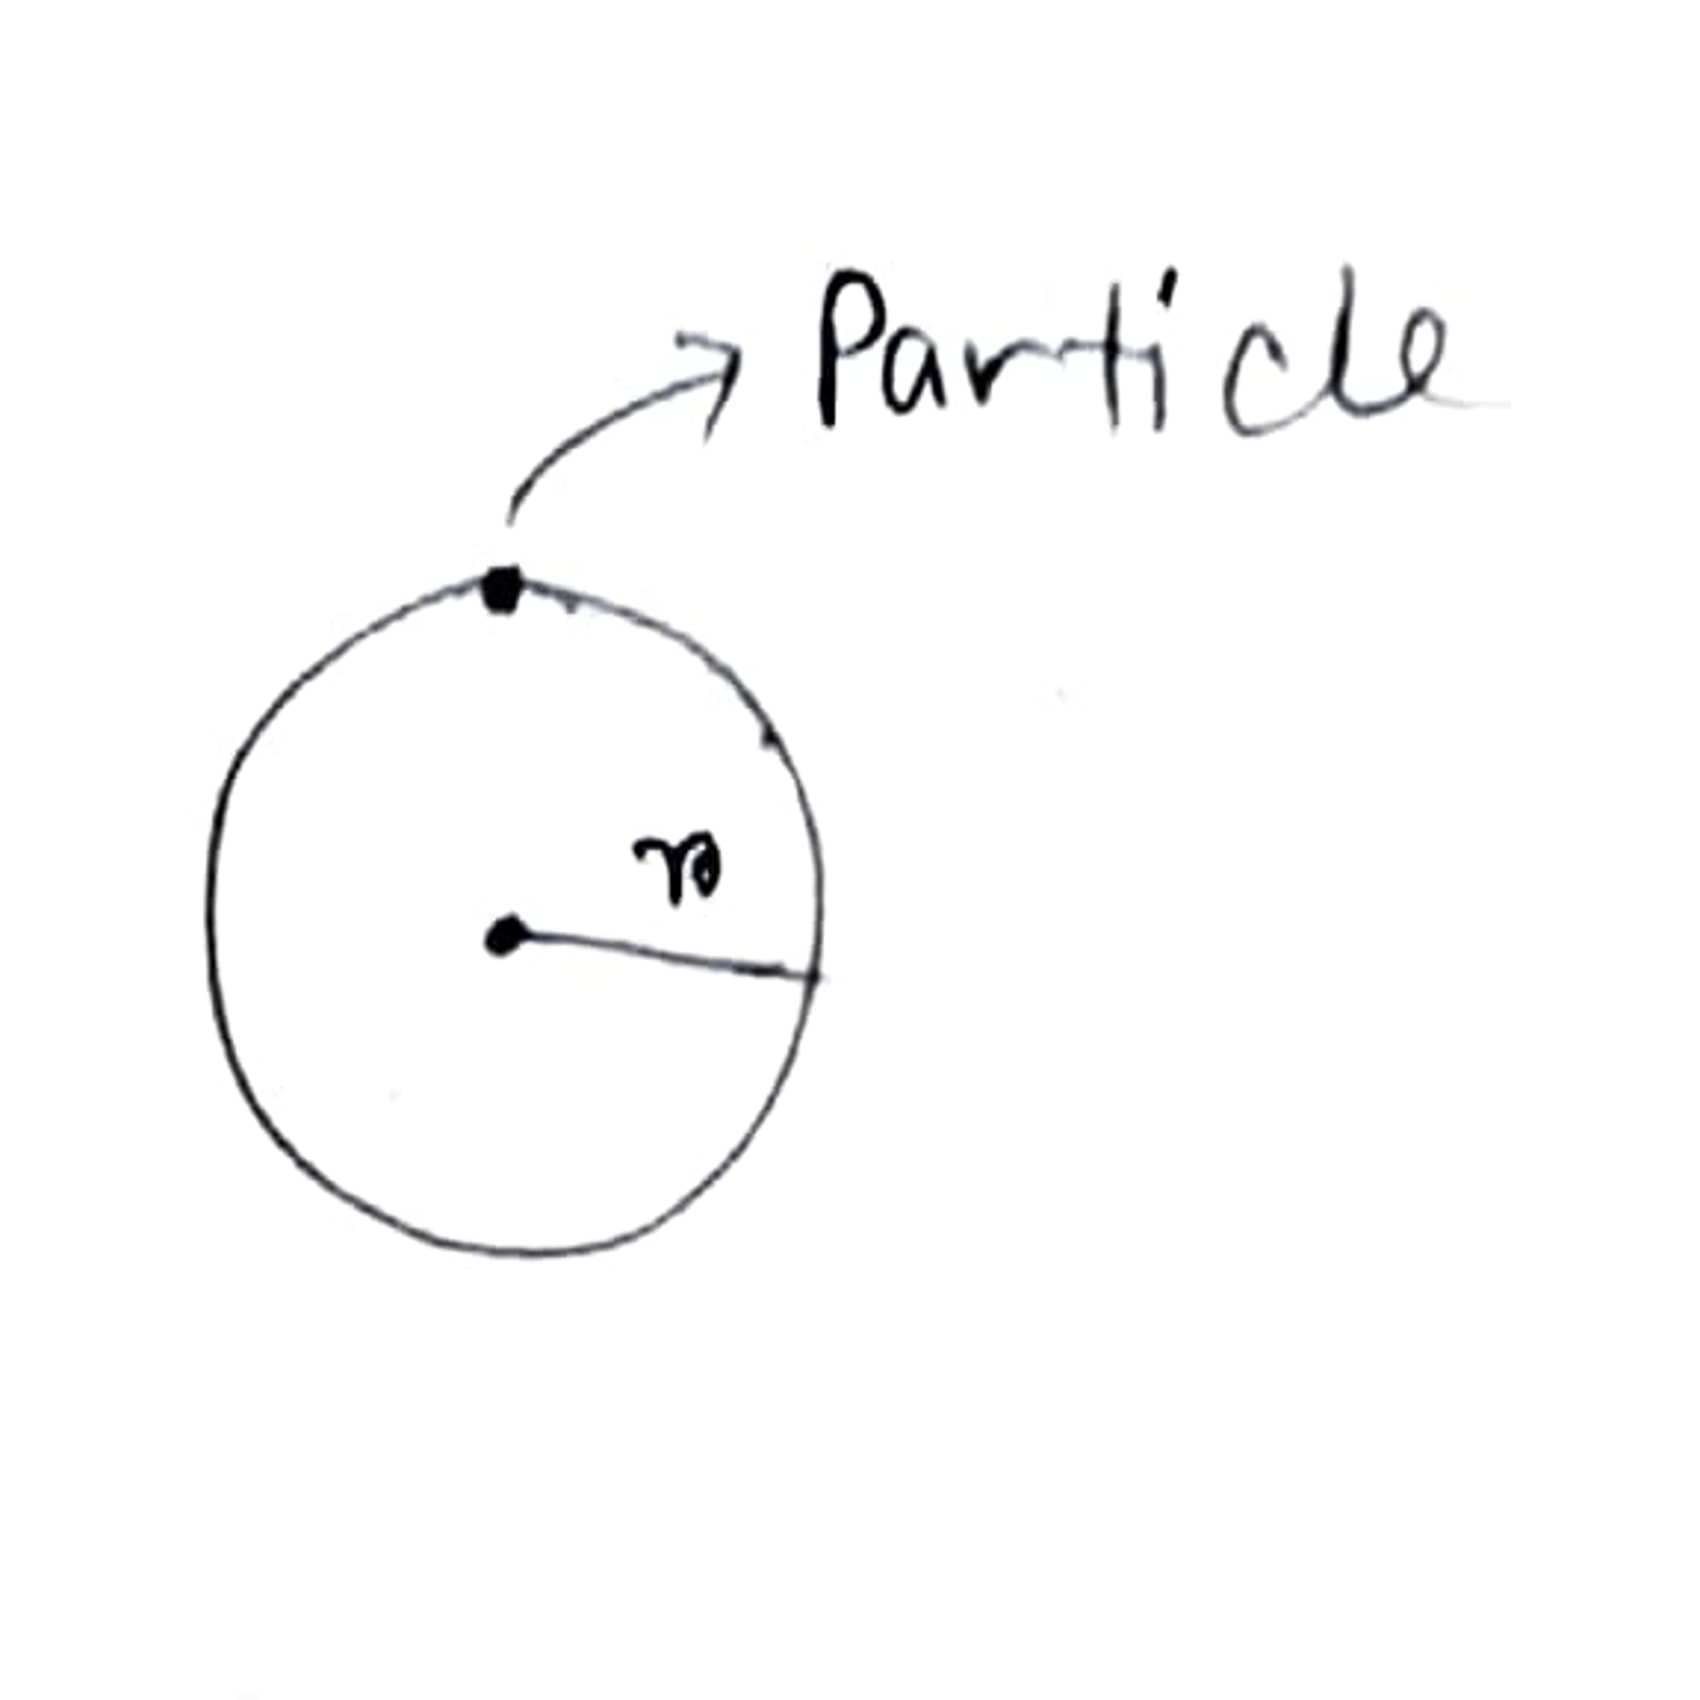
\includegraphics[width=0.3\linewidth]{L0_2 (1).jpg}
\caption*{}
\end{figure}
\vspace{-1.6cm}
% ---
For a particle on a circle, we can immediately write the  Lagrangian of the system:
\[
L = T - V(x,y)= \frac{1}{2}m\left( \dot{x}^2 + \dot{y}^2 \right) - V(x,y) \tag{6} \label{eq:6}
\]
Now, following the procedures:
\begin{enumerate}
    \item Constraint: \quad $\phi(x,y) = x^2 + y^2 - r^2 = 0$
    \item Promoting variables to operators:
\[
    x \rightarrow \hat{x}, \quad y \rightarrow \hat{y}, \quad p \rightarrow \hat{p}_i = -i \partial_i
\]
    \item Similar with constraint: 
\[
    \phi(x,y) \rightarrow \hat{\phi}(\hat{x},\hat{y}) = \hat{x}^2 + \hat{y}^2 - r^2 = 0
\]
    Also, to incorporate the constraint into the Lagrangian, we need Lagrange's multiplier, i.e.,
\[
L = \frac{1}{2} m (\dot{x}^2 + \dot{y}^2) - V(x,y) + \lambda \left(\neq x,y)(\dot{x}^2 + \dot{y}^2) - m^2 \right)
\]
$$ \text{(\textbf{Note:} $\lambda$ is not a function in this case.)} $$
\begin{itemize}
\item If $\lambda$ is a function of (x,y), then the derivative of it needs to be considered too. But we want no dynamics of the system due to this multiplier. In that case,
\[
\frac{\partial \mathcal{L}}{\partial \lambda} = 0
\]
Hence, $p = 0$, no evolution due to $\lambda$ exists!
\end{itemize}
    
    \item Therefore, Hamiltonian will be:
    \begin{align*}
        H = \frac{1}{2m}\left( p_x^2 + p_y^2 \right) + V(x,y) \tag{7} \label{eq:7} \\
        \hat{H} = \frac{1}{2m}\left( \hat{p}_x^2 + \hat{p}_y^2 \right) + \hat{V}(x,y) \\
        \Rightarrow \hat{H} = \frac{-1}{2m}\left( \partial_x^2 + \partial_y^2 \right) + \hat{V}(x,y)
    \end{align*}
\end{enumerate}
Now, imposing constraints on the state:
\[
\hat{\phi}(\hat{x},\hat{y}) \, \psi(x,y) = 0
\]
\[
\Rightarrow \left( \hat{x}^2 + \hat{y}^2 - r^2 \right) \psi(x,y) = 0
\]

i.e., if the constraint is satisfied, the allowed states (or values) form a subset of the full space.

$$ \textbf{We can use this formalism to quantize the system of a point particle.} $$
\subsection*{Klein Gordon (KG) equation:}
Now, using equation \eqref{eq:5}, i.e.,
\[
p^2 = m^2 \quad \Rightarrow \quad \text{constraint} \quad \hat{\phi} = \hat{p}^2 - m^2 = 0
\]
a.k.a. Schrödinger correspondence.

Imposing constraint on the state:
\begin{align*}
    (\hat{p}^2 - m^2) \, \psi(x) = 0 \\
    \Rightarrow - (\partial^2 + m^2) \psi(x) = 0
\end{align*}
$$ \text{The KG (Klein-Gordon) equation!} $$
% ---
\subsection{Action for Massless Particle}
From equation \eqref{eq:1}, we get:
\[
S = m \int d\tau
\]
(It wasn't first recognized as mass, but later leveled as mass from the constraint $p^2 = m^2$.)\\

Now, if $m=0$, $S=0$; action vanishes!\\

Then, the equivalent way to get around this problem is to define a new action:

\[
S = \frac{1}{2} \int \left[ \frac{1}{e} \dot{x}^2 + e m^2 \right] d\tau =\int \mathcal{L}~ d \tau \tag{8} \label{eq:8}
\]
where $e$ is a Lagrange multiplier and does not propagate to the equations of motion.
% ---
\subsection*{Equation of motion for $e$ :}
\begin{align*}
    & \quad\quad~~\frac{d}{d\tau} \frac{\partial \mathcal{L}}{\partial \dot{e}} - \frac{\partial \mathcal{L}}{\partial e} = 0 \\
    & \Rightarrow -\frac{\partial}{\partial e} \left[ \frac{1}{e} \dot{x}^2 + e m^2 \right] = 0 \\
    & \Rightarrow -\left( -\frac{1}{e^2} \dot{x}^2 + m^2 \right) = 0 \\
    & \quad\quad\therefore \quad e = \frac{\sqrt{\dot{x}^2}}{m}
\quad \tag{9} \label{eq:9}
\end{align*}
Putting in equation \eqref{eq:8},
\begin{align*}
    S &= \frac{1}{2} \int \left( \frac{m}{\sqrt{\dot{x}^2}} \dot{x}^2 + \frac{\sqrt{\dot{x}^2}}{m} m^2 \right) d\tau \\
    &= \frac{1}{2} \int 2m \sqrt{\dot{x}^2} \, d\tau \\
    &= m \int \sqrt{\dot{x}^2} \, d\tau \tag{10} \label{eq:10}
\end{align*}
and
\[
p_a = \frac{\partial \mathcal{L}}{\partial \dot{e}} = \frac{\dot{x}}{e} \tag{11}
\label{eq:11}
\]
\subsection*{Hamiltonian}
\begin{align*}
    H &= p_a \dot{x}^a - \mathcal{L} \\
    &= \frac{\dot{x}}{e} \dot{x} - \frac{1}{2} \left( \frac{\dot{x}^2}{e} + e m^2 \right) \\
    &= \frac{\dot{x}^2}{e} - \frac{\dot{x}^2}{2e} - \frac{e m^2}{2} \\
    &= \frac{1}{2} e \left( \frac{\dot{x}^2}{e^2} - m^2 \right) \\
    \therefore~H &= \frac{1}{2} e \left( p_a^2 - m^2 \right) \tag{12}
\end{align*}
i.e., Hamiltonian is proportional to the constraint of the system:
\[
H \propto \left( p_a^2 - m^2 \right)
\]
It means that the Hamiltonian vanishes ``on-shell," that is, when the constraints are satisfied. That is when real time evolution disappears. \\
% ---
\textbf{Extra:}
Generic form of Schrödinger equation is:
\[
i\hbar \frac{\partial \psi}{\partial t} = H \psi
\]
\begin{itemize}
\item H will change according to the system.
\item In Cartesian coordinates, one particular form is
\[
\left( -\frac{\hbar^2}{2m} \nabla^2 + V \right) \psi = H \psi = i \hbar \frac{\partial \psi}{\partial t}
\]
\item But in spin systems, the Hamiltonian will be
\[
H = \mu \, \vec{B} \cdot \vec{S}
\]
\end{itemize}
\newpage

%-------------------------------
% Section: Lecture 1
%-------------------------------

\stepcounter{section}
\renewcommand{\thesection}{\arabic{section}}
\fancysection{(\textit{\textbf{Class-4})} Lecture \textbf{1}: Sat, May 17, 2025}{\textbf{\textit{Poincaré Algebra}}}
Previously we've seen the Lagrangian for the massive and massless particles are -
\begin{align*}
L &= M \sqrt{\dot{x_p}~\dot{x^p}} \quad \quad~~~~~\text{(massive)}\\
L &= \frac{1}{2}(\frac{1}{e}\dot{x}^2- em^2) \quad \text{(massless)}
\end{align*}
These two are equivalent ``on-shell" condition . \textbf{On-shell} means a particle or field satisfies its equation of motion - usually the relativistic energy momentum relation: $E^2 = \vec{p}~^2+m^2$ \\

So a particle is on shell if: $p^\mu p_\mu = m^2$
This is called the \textbf{mass-shell condition}.

% ---
\begin{tcolorbox}[ title=\textbf{Question: What is a particle?}]
% \vspace*{-0.5cm}
Particle is something that carries a unitary representation of the Poincaré group.
\end{tcolorbox}
% ---
\begin{tcolorbox}[ title=\textbf{Question: What is Lorentz transformation?}]
A Lorentz transformation is a linear transformation that preserves the Minkowski spacetime interval-
\[
\eta_{\mu \nu} ~x^\mu x^\nu = \eta_{\rho \sigma} ~x^\rho x^\sigma 
\]
That is,
\[
x'^{\mu} = \Lambda^{\mu}~_{\nu}~x^\nu \quad;\quad \text{ such that,}\quad \Lambda^\top \eta~ \Lambda=\eta
\]
Notes -
\begin{itemize}
    \item The origin is invariant in the transformation. 
    \item Rotation is also a linear transformation where origin is kept invariant
\end{itemize}
\end{tcolorbox}
% ---
\subsection{Poincaré transformation}
Here the requirement that the origin remain invariant is relaxed, allowing transformations that preserve the interval between any two points including translation also. \\

Linear transformation which leaves the distance square between any two points invariant constitute Poincaré transformation. It is also a group.
% ---
\begin{tcolorbox}[ title=\textbf{Question: What are groups? \hfill (set + binary operation)}]
A group is denoted by $(G,*)$ is set of objects denoted $G$ and some operation on those objects denoted *, subject to the following -
\begin{align*}
&\bullet~\text{Associative} \quad \bullet~\text{Inverse} \\
&\bullet~\text{Close Set} \quad ~~~\bullet~\text{Existence of Identity }
\end{align*}
\end{tcolorbox}
% ---
\subsection{Poincaré/Affined group}
Poincaré group = Lorentz group + Translation 
= Rotation + Boosts + Translation 
\[
x^m \rightarrow x'~^m = (\Lambda x)^m + a^m = \Lambda^{m}~_{n}~x^n + a^m
\]
\begin{align*}
    \text{Here,} \quad (\Lambda, a) &\rightarrow \text{set of elements} \quad  \therefore x' = (\Lambda, a)x \\
    \Lambda &= \text{Lorentz matrix} \\
    a &= \text{Translation vector}
\end{align*}

\subsubsection*{(i) Associativity}
\vspace{-0.7cm}
\begin{align*}
    x' &= \Lambda x + a \\
    \Rightarrow x &= \Lambda^{-1} (x' - a) \\
    \Rightarrow x &= \Lambda^{-1} x' -  \Lambda^{-1}a \\
    \therefore (\Lambda&, a)^{-1} = (\Lambda^{-1}, -\Lambda^{-1}a) \tag{4.1} \label{eq:4.1}
\end{align*}
\begin{tcolorbox}[ title=\textbf{Note:}]

Is the space-time position operator $(x^a)$ a well-defined operator or observable in relativistic quantum theory? 

\medskip

\noindent \textbf{No, it is not.} Therefore, relativistic quantum mechanics in the usual sense does not exist — only \textit{relativistic quantum field theory (QFT)} exists. This is because:

\begin{itemize}
    \item [1.] In non-relativistic quantum mechanics (NQRM), the position operator $\hat{x}$ is well-defined. A particle can be localized in space and the wavefunction $\psi(x,t)$ gives the probability amplitude for the particle's position.
    
    \item [2.] In relativistic quantum mechanics (RQM), trying to promote space-time coordinates, $x^a = (t, \vec{x})$, to operators runs into problems due to:    
    \begin{itemize}
        \item Time and space do not enter symmetrically as operators — time is treated as a parameter, not as an operator.
    \end{itemize}
\end{itemize}

\noindent Therefore, only \textbf{relativistic quantum fields} exist, where the fundamental objects are fields $\hat{\phi}(x)$ — operator-valued functions over space-time.
$$\textbf{Observables are constructed from fields, not from position operators.}$$
\end{tcolorbox}

\subsubsection*{(ii) Identity}
\vspace{-0.7cm}
\[
x' = x(\mathbb{I},a)
\]

\subsubsection{Group Composition}
In Poincaré group, group composition refers to how two Poincaré transformations combine when applied one after the other.
Now, the Lorentz transformation is,
$$x'^\mu = \Lambda^\mu~_\nu~x^\nu + a^\mu ~ ; ~\Lambda^\mu~_\nu \in \text{SO}(1,3)$$
Poincaré transformation is denoted as a pair, $(\Lambda, a)$. Meaning,
\begin{itemize}
    \item [1.] Apply Lorentz transformation, $\Lambda$ 
    \item [2.] Then translate by $a$
\end{itemize}
Law: 
Given two transformations,
$$
(\Lambda_1, a_1)=(\Lambda, a)~;~(\Lambda_2, a_2)=(\Lambda', a')
$$
Their composition [do $(\Lambda', a')$ after $(\Lambda, a)$] is,
\begin{align*}
    (\Lambda', a')(\Lambda, a)x &= (\Lambda', a')(\Lambda x, a) \\
                                &= \Lambda'(\Lambda x+a) + a' \\
                                &= \Lambda'\Lambda x+\Lambda' a + a' \\
  \therefore (\Lambda', a')(\Lambda, a) &= (\Lambda'\Lambda,\Lambda' a + a') \tag{4.2} \label{eq:4.2}
\end{align*}
Applying matrices R: 
\[R(\Lambda', a')R(\Lambda, a) = R(\Lambda'\Lambda,\Lambda' a + a') \tag{4.3} \label{eq:4.3}
\]
%  ---
\begin{tcolorbox}[ title=\textbf{Question: Why Unitary representation}]
\textit{Eugene Wigner} classified all possible elementary particles in terms of irreducible unitary representations of the Poincaré group. These representations are labeled by:
\[
\bullet ~\text{Particle's mass}\quad \bullet ~\text{Particle's spin}
\]
We need unitary representations because of \textit{the preservation of probability}. In quantum mechanics, we don't perform transformations on $x$ directly, but on a wavefunction $\psi(x)$:
\[
\psi'(x) = U(x)\psi(x) = \psi(x+a)
\]
Then, if $\langle \psi | \psi \rangle = \langle \psi' | \psi' \rangle$, transformations are required to be unitary.
\end{tcolorbox}
%  ---
Therefore the unitary representation must satisfy \eqref{eq:4.3} -
\[
U(\Lambda', a')U(\Lambda, a) = U(\Lambda'\Lambda,\Lambda' a + a') \tag{4.4} \label{eq:4.4}
\]
\begin{tcolorbox}[ title=\textbf{Note: Dimension of Unitary Transformation in Hilbert Space}]
In Hilbert space, unitary transformations are not restricted to infinite dimensions. They can be finite or infinite dimensional depending on the physical system:

\begin{itemize}
    \item Finite-dimensional unitary representations arise in systems with discrete bases — for example, spin systems where spin states form a finite-dimensional Hilbert space.
    \item Infinite-dimensional unitary representations are necessary for systems with continuous degrees of freedom — such as position and momentum representations in quantum mechanics.
\end{itemize}
\end{tcolorbox}
Now, $U^\dagger U = \hat{\mathbb{I}}$ ; If isomorphic and acts on Hilbert space.
\begin{align*}
    \text{If}\quad &gg'=g'' \quad \text{and} \quad gg^{-1}=\mathbb{I} \\
    \text{Then} \quad & U(g)U(g') = U(g'') \quad \text{and} \quad U(g)U(g^{-1}) = U(\mathbb{I}) = \hat{\mathbb{I}} \\
    &\therefore U(g^{-1}) = U^{\dagger}{(g})\\
    &\therefore U^\dagger(\Lambda,a)=U\left((\Lambda,a)^{-1}\right)=U(\Lambda^{-1},-\Lambda^{-1}a)  \tag{4.5} \label{eq:4.5}
\end{align*}
This transformation acts on space time.
\begin{figure}[H]
\centering
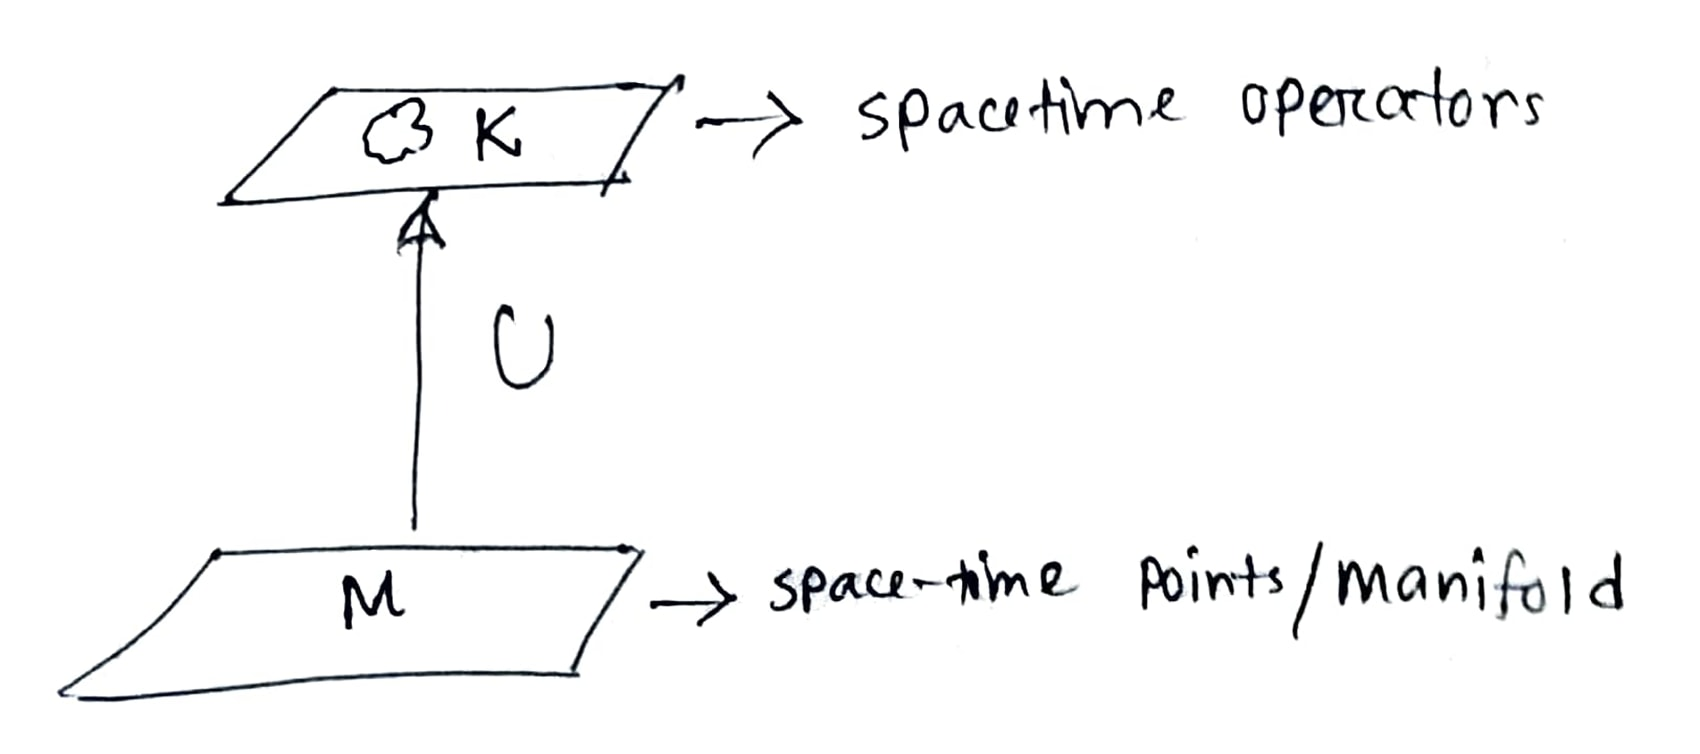
\includegraphics[width=0.6\linewidth]{L1_1.jpg}
\caption*{}
\end{figure}
\begin{tcolorbox}[ title=\textbf{Notes:}]
\textbf{Group Representation}
\vspace{0.1cm}
\newline
When studying symmetry transformations, we represent them using matrices that act on a vector space.  
The collection of such matrices that preserves the group structure is called a \textit{representation} of the group.  
The space on which these matrices act is known as the \textit{representation space}.
\vspace{0.1cm}
\newline
\textbf{Irreducible Representation:}  
A representation is called irreducible if it has no proper, non-trivial invariant subspace.

\vspace{0.1cm}
\textbf{Invariant Subspace:}  
Let $T: V \rightarrow V$ be a linear operator on a vector space $V$. A subspace $W \subseteq V$ is called *invariant* under $T$ if:
\[
\forall w \in W,\quad T(w) \in W
\]
That is, applying $T$ to any vector in $W$ keeps it inside $W$.

\vspace{0.3cm}
\textbf{Similarity Transformation}

A similarity transformation rewrites a matrix $A$ in a different basis using an invertible matrix $S$:
\[
A' = S A S^{-1}
\]
Key properties:
\begin{itemize}
    \item[(i)] $A$ and $A'$ are similar matrices; they represent the same linear transformation in different bases.
    \item[(ii)] They have identical eigenvalues, trace, and determinant.
\end{itemize}

\textbf{Example:} If $AB = C$, then under similarity transformation:
\begin{align*}
A'& =SAS^{-1} \\
B' &= SBS^{-1} \\
    \therefore A'B' &= (SAS^{-1})(SBS^{-1}) = S(AB)S^{-1} = SCS^{-1} = C'
\end{align*}

Thus, $C'$ is the similarity transformation of $C$.
\vspace{0.3cm}

\textbf{Conjugation of a Group Element:}
\newline
If $B' = SBS^{-1}$, we call $B'$ the \textit{conjugate} of $B$ by $S$.
This does not imply a group product, it’s a transformation under a change of basis.
\end{tcolorbox}
% ===
\noindent
Back to Wigner, recall \eqref{eq:4.4} and \eqref{eq:4.5} ,
\[
U(\Lambda', a')U(\Lambda, a) = U(\Lambda'\Lambda,\Lambda' a + a') \tag{4.4}
\]
\[
U^\dagger(\Lambda,a)=U\left((\Lambda,a)^{-1}\right)=U(\Lambda^{-1},-\Lambda^{-1}a)  \tag{4.5}
\]
Using both the equations we get,
\begin{align*}
U(\Lambda, a) U(\Lambda', a') U^\dagger(\Lambda, a)
&= U(\Lambda \Lambda', \Lambda a' + a) U(\Lambda^{-1}, -\Lambda^{-1} a) \\
&= U(\Lambda \Lambda' \Lambda^{-1}, \Lambda \Lambda' (-\Lambda' a) + \Lambda a' + a) \\
&= U(\Lambda \Lambda' \Lambda^{-1}, \Lambda a' + (\mathbb{I} - \Lambda \Lambda' \Lambda^{-1}) a) \tag{4.6} \label{4.6}
\end{align*}
Then by combining \eqref{eq:4.1} and \eqref{eq:4.2} we get,
\begin{align*}
\quad~(\Lambda, a) (\Lambda', a') (\Lambda, a)^{-1} 
&\equiv (\Lambda \Lambda', \Lambda a' + a) (\Lambda', -\Lambda' a) \\
&= \Lambda \Lambda' \Lambda^{-1}, \Lambda \Lambda' (-\Lambda' a) + \Lambda a' + a \\
&= \Lambda \Lambda' \Lambda^{-1}, \Lambda a' +a - \Lambda \Lambda' \Lambda^{-1} a \\
&= \left( \Lambda \Lambda' \Lambda^{-1}, \Lambda a' + (\mathbb{I} - \Lambda \Lambda' \Lambda^{-1}) a \right) \tag{4.7} \label{4.7}
\end{align*}
Now, the theory of Lie groups tells us that we can write any unitary matrix in the form:
\[
U(\theta) = e^{ i \vec{\theta}\cdot \vec{H} } \quad, \quad \theta=(\theta_1, \theta_2, \dots),\ H=(H_1, H_2, \dots)
\]
where $\vec{\theta}$ and $\vec{H}$ are vectors of parameters and Hermitian operators, respectively.  
This form holds under the assumption: $U(0) = \hat{\mathbb{I}}$
$$ \boxed{\textbf{Unitary transformation transforms the additive space to multiplicative space.}} $$
\begin{figure}[H]
\centering
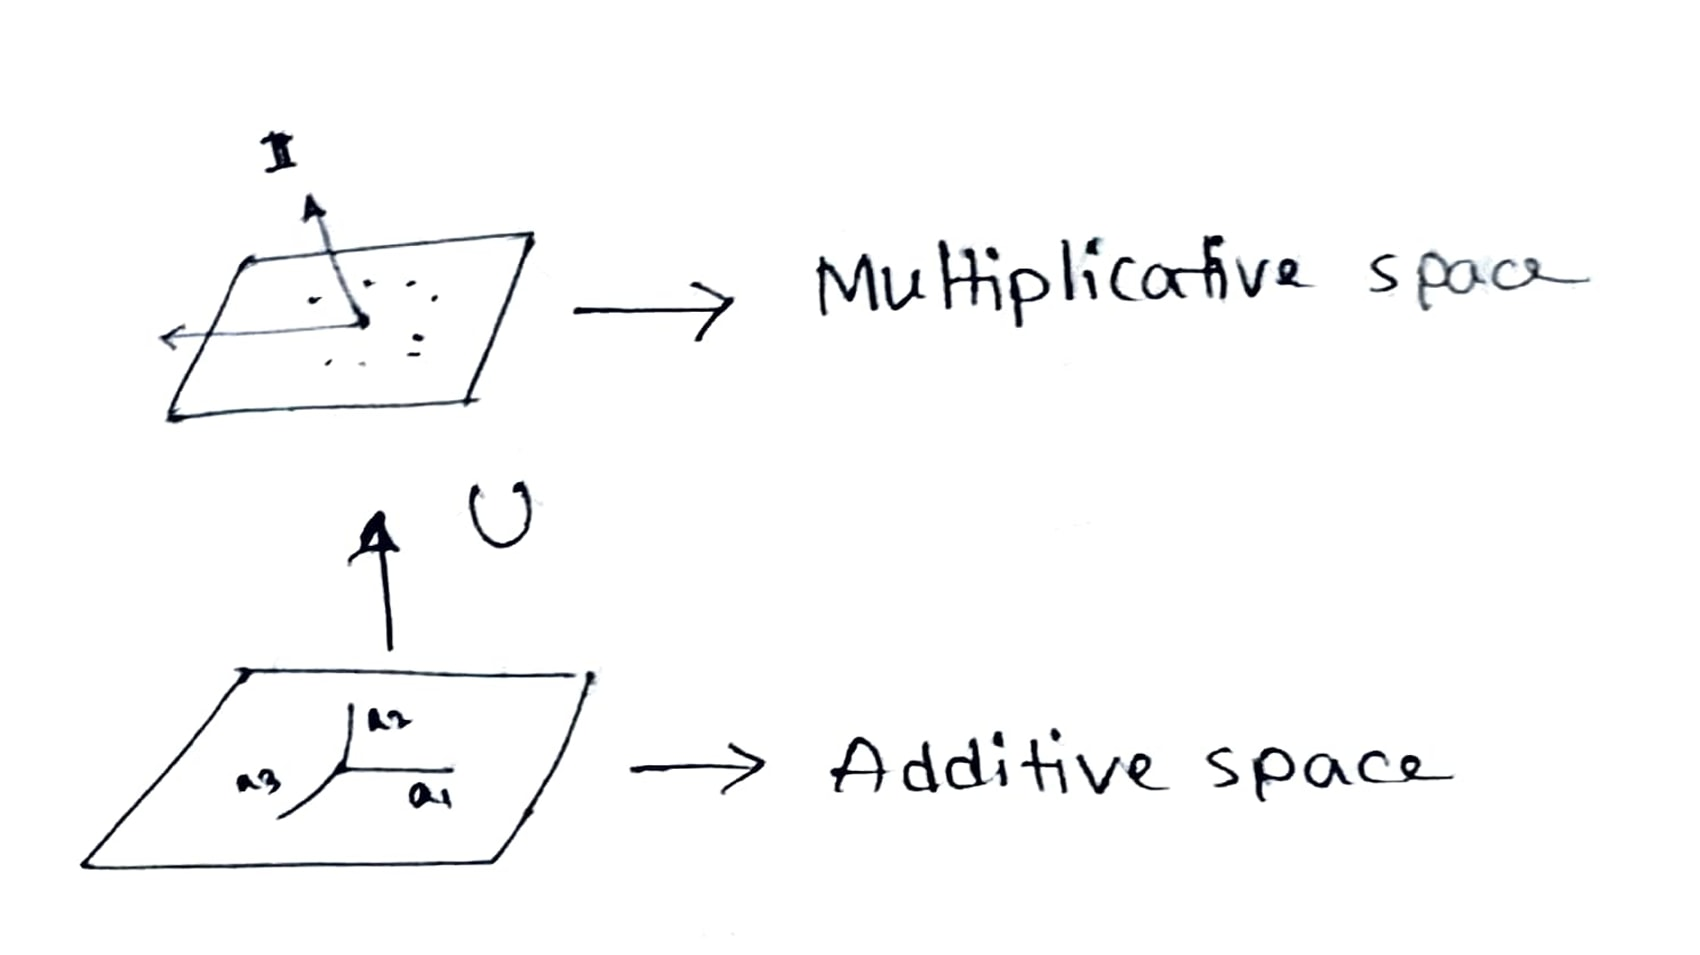
\includegraphics[width=0.7\linewidth]{L1_2.jpg}
\caption*{}
\end{figure}
\begin{tcolorbox}[ title=\textbf{Note}]
It is also possible for $U = -\hat{\mathbb{I}}$, since
\[
U^\dagger U = \mathbb{I}
\]
However, this does \textbf{not} satisfy the condition $U(0) = \hat{\mathbb{I}}$ and therefore cannot be expressed in the exponential form $e^{ i \vec{\theta}\cdot\vec{H}}$.
\end{tcolorbox}
\noindent
Now for small $\theta,~U(\theta)$ can be Taylor expanded-
\[
U(\theta) = \hat{\mathbb{I}} + i ~\vec{\theta}\cdot \vec{H} + \dots
\]
Now evaluation of the wave function can be written as the form-
\begin{align*}
\psi(x + a) &= e^{a \frac{d}{dx}} \psi(x) = \left(1 + a \frac{d}{dx} + \cdots \right) \psi(x) \\
\Rightarrow \psi(x + a) &= e^{\frac{ia}{\hbar} (-i \hbar \frac{d}{dx})} \psi(x) \\
\end{align*}
Also for rotations we know that,
\[
R^\top R = R^\top \mathbb{I} R = \mathbb{I}
\]
and for Lorentz transformation,
\[
\Lambda^\top \eta~ \Lambda = \eta
\]
\begin{align*}
\text{Let,}\quad R &= \mathbb{I} + \epsilon W \\
R^\top &= \mathbb{I} + \epsilon W^\top
\end{align*}
for small transformations where, $\epsilon =$ number, $W=$ matrix that generates the rotation. It belongs to the Lie algebra of the rotation group SO(n).
\begin{align*}
\therefore R^\top R &= (\mathbb{I} + \epsilon W^\top)(\mathbb{I} + \epsilon W) \\
&= \mathbb{I} + \epsilon(W^\top + W) + \epsilon^2 W^\top W 
\end{align*}
Lie theory says that the substantial structure of group is encoded in its first order infinitesimals. So, $\epsilon^2 \rightarrow0$.And $R^\top R = \mathbb{I}$ implies that-
\[
W = -W^\top \quad \text{(Antisymmetric)}
\]
In $d$ dimensions, $d \times d = d^n$ parameters, main diagonal constitute of 0. Therefore independent $d^n -d$, lower and upper triangular part have the same input except the sign.
% Traceless matrix
Hence number of the independent parameters are-
\[
\frac{d^2 -d }{2} = \frac{d(d-1)}{2} = ~^d\mathbf{C}_2
\]
Then the affine or, Poincaré group has 
\[
(\Lambda,a) \rightarrow \frac{d(d-1)}{2} + 1 = \frac{d(d+1)}{2} \quad \text{dimensions}
\]
\begin{center}
    \textbf{This looks like rotation in $(d + 1)$ dimensions!}
\end{center}

\noindent Now for Poincaré transformation,
\begin{align*} 
&x' = \Lambda x + a \quad;\\
[~\Lambda \rightarrow \text{Multiplicative} &\text{(only for rotations)},~a \rightarrow \text{additive}~]
\end{align*}
Therefore, for the $(d + 1)$ dimensional rotation it can be written as in $2D$:
\[
\begin{pmatrix}
x' \\
1
\end{pmatrix}
=
\begin{pmatrix}
\Lambda & a \\
0 & 1
\end{pmatrix}
\begin{pmatrix}
x \\
1
\end{pmatrix}
\quad;\quad\left[
\begin{pmatrix}
x \\
1
\end{pmatrix}
\to
\begin{pmatrix}
d \rightarrow \text{ number of dimensions} \\
1 \rightarrow 3^{rd} \text{ dimension: } z \text{ is fixed} 
\end{pmatrix}
\right]
\]
It implies the idea that ``rotating in higher dimensions'' can relate to translation in lower dimensions. $\textbf{for example:}$  The rotation of laser points in $2D$ plane. When projected, it results in an apparent translation along the $z$ axis. \\

Now let Lorentz transformation be:
\begin{align*}
\Lambda' &= \mathbb{I}+W' \tag{4.8} \label{4.8} \\
\therefore U(\Lambda',a') = U(\mathbb{I}+& W',a') = \hat{\mathbb{I}} + i~a'\hat{P} + \frac{i}{2} W_{mn}~ \hat{J}^{mn} \tag{4.9} \label{4.9}
\end{align*}
\begin{align*}
\text{here, }&\frac{1}{2} \rightarrow\text{factor here is to avoid double counting}\\
&\quad \quad \quad \text{as } W_{mn} \text{ is antisymmetric matrix}\\
&\hat{P} \rightarrow \text{an operator whether it is translational}\\ &\quad \quad \quad\text{or not will be given by its } \textbf{``Algebra''} \\
W_{mn} &= -W_{nm} \quad;\quad \hat{J}^{mn} = -\hat{J}^{nm} \quad;\quad a' = \text{a number}
\end{align*}
Let's get back to Wigner once more. Using equation \eqref{4.8} in $\Lambda \Lambda' \Lambda^{-1}$ we get,
% \begin{align*}
% \Lambda \Lambda' \Lambda^{-1} = \Lambda (\mathbb{I}+W')\Lambda^{-1} &=\mathbb{I} + \Lambda W' \Lambda^{-1} \tag{4.10} \label{4.10}\\
% \text{and, } \Lambda a'+(\mathbb{I}-\Lambda \Lambda' \Lambda^{-1})a &= \Lambda a'-\Lambda \Lambda' \Lambda^{-1}a - \Lambda W' \Lambda^{-1} \tag{4.11} \label{4.11}
% \end{align*}
\begin{align*}
\Lambda \Lambda' \Lambda^{-1} = \Lambda (\mathbb{I}+W')\Lambda^{-1} &=\mathbb{I} + \Lambda W' \Lambda^{-1} \tag{4.10} \label{4.10}\\
\text{and, } \Lambda a'+(\mathbb{I}-\Lambda \Lambda' \Lambda^{-1})a &= \Lambda a' - \Lambda W' \Lambda^{-1}a \tag{4.11} \label{4.11}
\end{align*}
Recall equation \eqref{4.6}:
\[
U(\Lambda, a) U(\Lambda', a') U^\dagger(\Lambda, a) = U(\Lambda \Lambda' \Lambda^{-1}, \Lambda a' + (\mathbb{I} - \Lambda \Lambda' \Lambda^{-1}) a) \tag{4.6} \label{4.6}
\]
Now combining equation \eqref{4.6}, \eqref{4.9}, \eqref{4.10}, \eqref{4.11} we will get:
\begin{align*}
&~~\therefore U(\Lambda, a) U(\Lambda', a') U^\dagger(\Lambda, a) = U(\Lambda, a) \left[ \hat{\mathbb{I}} + i~a'\hat{P} + \frac{i}{2} W_{mn} ~\hat{J}^{mn} \right] U^\dagger(\Lambda, a) \\
&\Rightarrow U\left(\Lambda \Lambda'\Lambda^{-1}, \Lambda a' + (\mathbb{I} - \Lambda \Lambda'\Lambda^{-1})a~ \right) = U(\Lambda, a)\left[\mathbb{I} + i a_n' \hat{P}^n + \frac{1}{2} W_{mn}~ \hat{J}^{mn}\right] U^\dagger(\Lambda, a) \\
&\Rightarrow U(\mathbb{I} + \Lambda W \Lambda^{-1}, \Lambda a - \Lambda W \Lambda^{-1}a) = U(\Lambda, a)\left[\mathbb{I} + i a_n' \hat{P}^n + \frac{1}{2} W_{mn}~ \hat{J}^{mn}\right] U^\dagger(\Lambda, a) \\
&\Rightarrow \mathbb{I} + i a_n' ~U(\Lambda, a) \hat{P}^n~ U^\dagger(\Lambda, a) + \frac{i}{2} W_{mn}~ U(\Lambda, a) \hat{J}^{mn}~U^\dagger(\Lambda, a) \\
& \quad \quad \quad= \mathbb{I} + i (\Lambda a'-\Lambda W \Lambda^{-1})_n ~\hat{P}^n + \frac{i}{2} (\Lambda W \Lambda^{-1})_{pq}~ \hat{J}^{pq} \tag{4.12}  \label{4.12}\\
&\Rightarrow\quad i a_n'~ U(\Lambda, a) \hat{P}^n~ U^\dagger(\Lambda, a) + \frac{i}{2} W_{mn} ~U(\Lambda, a) \hat{J}^{mn}~ U^\dagger(\Lambda, a) \\
& \quad \quad \quad= i {(\Lambda a')}_n \hat{P}^n + \frac{i}{2} {(\Lambda W \Lambda^{-1})}_{pq} \hat{J}^{pq} -i(\Lambda W \Lambda^{-1})_n~\hat{p}^n \tag{4.13}  \label{4.13}
\end{align*}
Now  matching the coefficients of $a'$ on both side of the equation \eqref{4.13},
\[
i ~a_n' ~U(\Lambda,a) \hat{P}^n ~U^\dagger(\Lambda, a) = i{(\Lambda a')}_m~\hat{P}^m = i~ \Lambda_m~^s~a_s'~\hat{P}^m = i~\Lambda_m~^n~a_n'~\hat{P}^m 
\]
\[
\boxed{\therefore U(\Lambda, a) \hat{P}^n~ U^\dagger(\Lambda, a) = \Lambda_m~^n\hat{P}^m}
\]
Thus we can see that, $\hat{P}$ transforms like a vector under the group. It is a constant matrix. It doesn't depend on the coordinates or the values of $a'$.
\begin{framed}
\noindent \textbf{Assignment-1:}\\
\noindent How does $\hat{J}^{rs}$ transform under Poincaré transformation? (It's a semi direct product)
\end{framed}
\vspace{-0.5cm}
\begin{tcolorbox}[ title=\textbf{Note:}]
\textbf{Direct Product and Semi-direct product}
\newline
In group theory, a direct product of two groups means that the groups combine in a way where elements of one group do not affect the operation of the other. That is:
\[
(a_1, b_1)(a_2, b_2) = (a_1 a_2, b_1 b_2)
\]
Here, two group elements become separated completely.\\
Poincaré group combines Lorentz transformations and spacetime translations as:
\[
(\Lambda', a')(\Lambda, a) = (\Lambda'\Lambda, \Lambda'a + a')
\]

Here, the second translation is transformed by $\Lambda'$, meaning the two parts interact nontrivially. Hence, this is not a direct product but a \textbf{semi-direct product}. The Lorentz part $\Lambda'$ transforms the translation $a$, indicating that the two subgroups are not independent.
\end{tcolorbox}
\vspace{-0.7cm}
\subsection*{Transformation of $\hat{J}^{pq}$ under Lorentz transformation}
Assume $a = 0 \equiv$ No translation under Lorentz transformation. From the equation \eqref{4.12},
\begin{align*}
&\mathbb{I} + i a_n' ~U(\Lambda, a) \hat{P}^n~ U^\dagger(\Lambda, a) + \frac{i}{2} W_{mn}' U(\Lambda, a) \hat{J}^{mn}~U^\dagger(\Lambda, a) \\
&= \mathbb{I} + i {(\Lambda a'-\Lambda W' \Lambda^{-1})}_n~\hat{P}^n + \frac{i}{2} {(\Lambda W' \Lambda^{-1})}_{pq}~\hat{J}^{pq}
\end{align*}
Putting $a=0$ and comparing the $2^{nd}$ term on both sides,
\begin{align*}
&~~~~~~ W_{pq}'~ U \hat{J}^{pq}~ U^\dagger = (\Lambda W' \Lambda^{-1})_{ab} \hat{J}^{ab} \\
&\Rightarrow W_{pq}'~ U \hat{J}^{pq}~ U^\dagger = \Lambda_a~^m~ W_{mn}'(\Lambda^{-1})^n{}_b \hat{J}^{ab} \\
&~~~~~~\text{By setting}~~ m=p,~n=q ~~;~\text{ we get,} \\
&\Rightarrow W_{pq}'~ U \hat{J}^{pq}~ U^\dagger = \Lambda_a~^p~ W_{pq}' ~(\Lambda^{-1})^q{}_b~ \hat{J}^{ab} \\
&\Rightarrow U \hat{J}^{pq}~ U^\dagger = \Lambda_a~^p (\Lambda^{-1})^q~_b \hat{J}^{ab} \tag{4.14} \label{4.14}
\end{align*}
Now, recall the Lorentz transformation,
\begin{align*}
\Lambda^\top \eta~&\Lambda = \eta \\
\Rightarrow \Lambda^\top \eta &~~~= \eta~\Lambda^{-1} \\
\therefore\eta ~\Lambda^\top \eta &~~~= \Lambda^{-1} \tag{4.15} \label{4.15}
\end{align*}
Putting this value of $\Lambda^{-1}$ in equation \eqref{4.14} we get,
\begin{align*}
U \hat{J}^{pq}~ U^\dagger &= \Lambda_a~^p (\eta ~\Lambda^\top \eta)^q~_b \hat{J}^{ab} \\
&= \Lambda_a~^p~\eta^q~_r~\Lambda^r~_s~\eta^s~_b \hat{J}^{ab}  \\
&= \Lambda_a~^p~\Lambda^q~_s~\hat{J}^{as} \\
&= \Lambda_a~^p~\Lambda^q~_b~\hat{J}^{ab}
\end{align*}
\[
\boxed{\therefore U \hat{J}^{pq}~ U^\dagger = \Lambda_a~^p~\Lambda^q~_b~\hat{J}^{ab}}
\]
Now substituting, $ U=e^{ \left( \frac{i}{2}W_{cd}~\hat{J}^{cd} \right) }$ and $\Lambda^p~_a = \delta^p~_a + W^p~_a $
Then,
\begin{align*}
& \quad \quad e^{ \left( \frac{i}{2}W_{cd}~\hat{J}^{cd} \right) } \cdot e^{ \left( -\frac{i}{2}W_{cd}~\hat{J}^{cd} \right) } = (\delta_a~^p + W^p~_a)(\delta^q~_b + W^p~_b) \hat{J}^{ab} \quad [\text{BCH Relation}]\\
&\Rightarrow \hat{J}^{pq} + \frac{i}{2} W_{cd} [\hat{J}^{cd}, \hat{J}^{pq}] = \left( \delta_a~^p \delta^q~_b + \delta_a~^p~W^p~_b + W^p~_a \delta^q~_b + W^p~_a W^p{}_b \right)~ \hat{J}^{ab} \\
&\Rightarrow \hat{J}^{pq} + \frac{i}{2} W_{cd} [\hat{J}^{cd}, \hat{J}^{pq}] = \hat{J}^{pq} + W^q{}_b \hat{J}^{pb} + W^p{}_a \hat{J}^{a q} \\
&\Rightarrow \frac{i}{2} W_{cd} [\hat{J}^{cd}, \hat{J}^{pq}] = W_{mb}~ \eta^{mq}~\hat{J}^{pb} + W_{na}~ \eta^{np}~\hat{J}^{aq} \\
&\Rightarrow \frac{i}{2} W_{cd} [\hat{J}^{cd}, \hat{J}^{pq}] = W_{cd}~ \eta^{cq}~\hat{J}^{pd} + W_{cd}~ \eta^{cp}~\hat{J}^{dq} \quad [b=d, m=c, a=d, n=c] \\
&\Rightarrow \frac{i}{2} W_{cd} [\hat{J}^{cd}, \hat{J}^{pq}] = W_{cd}\times\frac{1}{2} \left( \eta^{cq}~\hat{J}^{pd} - \eta^{dq}~\hat{J}^{pc} \right) + W_{cd}\times\frac{1}{2} \left( \eta^{cp}~\hat{J}^{dq} - \eta^{dp}~\hat{J}^{cq} \right) \\
& \quad \quad \left[ \text{Here we used, }\quad AB = \frac{1}{2}(AB + BA) + \frac{1}{2}(AB - BA) ~\right] \\
& \quad \quad \text{ Omitting } W_{cd} \text{ on both sides,}\\
&\Rightarrow [\hat{J}^{cd}, \hat{J}^{pq}] = -i~\left( \eta^{cq}~\hat{J}^{pd} - \eta^{dq}~\hat{J}^{pc} + \eta^{cp}~\hat{J}^{dq} - \eta^{dp}~\hat{J}^{cq} \right) \\
& \therefore [\hat{J}^{cd}, \hat{J}^{pq}] = -i~\left( \eta^{cq}~\hat{J}^{pd} - \eta^{dq}~\hat{J}^{pc} + \eta^{pc}~\hat{J}^{dq} - \eta^{pd}~\hat{J}^{cq} \right)
\end{align*}
\subsubsection*{Summary}
Here we have successfully found the algebra of angular momentum without the relation $\hat{J} = \vec{r} \times \vec{p}$, just simply using the algebra of the Poincaré group.\\

In addition, we know in $3D, \quad \hat{J}^m = i~\epsilon^{amn} \hat{J}_{a}$
\begin{framed}
\textbf{Assignment-2:} Recover $3D$ rotation algebra from angular momentum.
\end{framed}
\newpage
%-------------------------------
% Section: Lecture 2
%-------------------------------
\stepcounter{section}
\renewcommand{\thesection}{\arabic{section}}
\fancysection{(\textit{\textbf{Class-5})} Lecture \textbf{2}: Sat, May 24, 2025}{\textbf{\textit{A Glimpse of GR via The Classical Field Theory }}}
%------------%
\subsection{Road to GR (General relativity is a classical field theory because no quantization is involved here)}
In freely falling coordinates (FFC), the line element is given by:
\begin{align*}
    ds^2 &= \eta_{ab}~d\xi^a d\xi^b \tag{5.1} \label{5.1} \\
    \text{Notation:} \quad 
    \eta_{ab} &: \text{Flat Minkowski metric} \\
    \xi^a &: \text{Freely falling coordinates (FFC)} \\
    x^a &: \text{General coordinates}
\end{align*}
%------------
\begin{tcolorbox}[ title=\textbf{Note:}]
\begin{itemize}
    \item In Special Relativity (SR), there is no representation of gravity.
    \item Only in curved space there is an existence of gravity hence acceleration arises.
\end{itemize}
\end{tcolorbox}
%-----------
\begin{figure}[H]
\centering
\includegraphics[width=0.4\linewidth]{figures/L2_1.jpg}
\caption*{}
\vspace{-1em}
\end{figure}
However, the FFC are locally defined as:
\begin{align*}
    \xi^a &= \xi^a(x) \\
    \Rightarrow d\xi^a &= \frac{\partial \xi^a}{\partial x^m}~ dx^m \tag{5.2} \label{5.2} \\
    \Rightarrow d\xi^a &\equiv M^a{}_m~dx^m \quad \text{(linear relation)}
\end{align*}
Substituting \eqref{5.2} into \eqref{5.1}, we get:
\begin{align*}
    ds^2 &= \eta_{ab}~\frac{\partial \xi^a}{\partial x^m} \frac{\partial \xi^b}{\partial x^n}~dx^m dx^n \tag{5.3} \label{5.3}
\end{align*}

\[\text{here,}\quad
\left[ \eta_{ab}~ \frac{\partial \xi^a}{\partial x^m} \frac{\partial \xi^b}{\partial x^n} \right] = \text{symmetric, depends on } x
\]

Let us define this term as:
\[
G_{mn}(x) \equiv \eta_{ab}~ \frac{\partial \xi^a}{\partial x^m} \frac{\partial \xi^b}{\partial x^n}
\]
Then:
\[
ds^2 = G_{mn}(x)~dx^m dx^n
\]
$G_{mn}(x)$ is called the metric which describes distance in a curved spacetime and has the following properties:
\begin{itemize}
    \item[1.] \textbf{Symmetry:} $G_{mn} = G_{nm}$
    \item[2.] \textbf{Non-degeneracy:} If $\det(G_{mn}) \neq 0$, then $G_{mn}$ is invertible.
\end{itemize}
Such a manifold is known as a \textit{Riemannian manifold} (or pseudo-Riemannian in Lorentzian spacetime).

\vspace{1em}
\noindent
\textbf{Action:} Recall the relativistic action:
\begin{align*}
    s &= m \int \sqrt{ \eta_{ab}~ \dot{\xi}^a \dot{\xi}^b } \, d\tau 
    \quad \text{(non-polynomial Lagrangian)} \\
    s' &= \frac{1}{2} \int \left( \frac{1}{e} \dot{\xi}^a \dot{\xi}^b~ \eta_{ab} - e m^2 \right) d\tau 
\end{align*}

\begin{itemize}
    \item First term in $s'$: kinetic term.
    \item Second term in $s'$: Lagrange multiplier (enforces mass-shell condition).
\end{itemize}

When $m = 0$, both $s$ and $s'$ are same, they yield the same dynamics.
%------------
\begin{tcolorbox}[ title=\textbf{Note:}]
For flat spacetime in Cartesian coordinates, the trajectory of a free particle is:
\[
x^i = x^i_0 + \left( \frac{p^i}{m} \right)t
\]
This equation -
\begin{itemize}
    \item is valid only in Cartesian coordinates and flat spacetime.
    \item has all quantities here carry upper indices (contravariant).
\end{itemize}

\vspace{1em}
\noindent
\textbf{Conjugate Momenta:}
\[
p_i = \frac{\partial \mathcal{L}}{\partial \dot{q}^i}
\]

\begin{itemize}
    \item $p_i$ and $q^i$ have different index positions because they live in dual spaces.
    \item The momentum $p_i$ lives in the \textbf{cotangent space} (dual vector space) to the configuration space.
\end{itemize}
\end{tcolorbox}
%-----------
Consider, for example, a scalar function: 
$$\phi(x) = \phi'(\xi)$$
where $x$ could be any coordinate system (e.g., spherical, Cartesian, etc.). Then,
\begin{align*}
    \frac{\partial \phi'(\xi)}{\partial \xi^a} 
    = \frac{\partial \phi(x)}{\partial x^m} \cdot \frac{\partial x^m}{\partial \xi^a} \tag{5.4} \label{5.4}
\end{align*}
Recall equation \eqref{5.3}:
\begin{align*}
    ds^2 = \eta_{ab}~ \frac{\partial \xi^a(x)}{\partial x^m} \frac{\partial \xi^b(x)}{\partial x^n}~ dx^m dx^n = G_{mn}(x)~ dx^m dx^n
\end{align*}
These equations \eqref{5.3} and \eqref{5.4} are inverse to each other — they reflect the transformation between coordinates and dual coordinates.
%------------
\begin{tcolorbox}[ title=\textbf{Note:}]
\subsubsection*{Phase Space}
\begin{itemize}
    \item The cotangent space of a manifold is called the \textbf{phase space}.
    \item The collection of all $x$ and $p$ coordinates also forms the phase space.
    \item The collection of all initial conditions again constitutes a phase space.
\end{itemize}
\end{tcolorbox}
%-----------
\subsection*{Differential and Gradient}
\vspace{-1cm}
\begin{figure}[H]
\centering
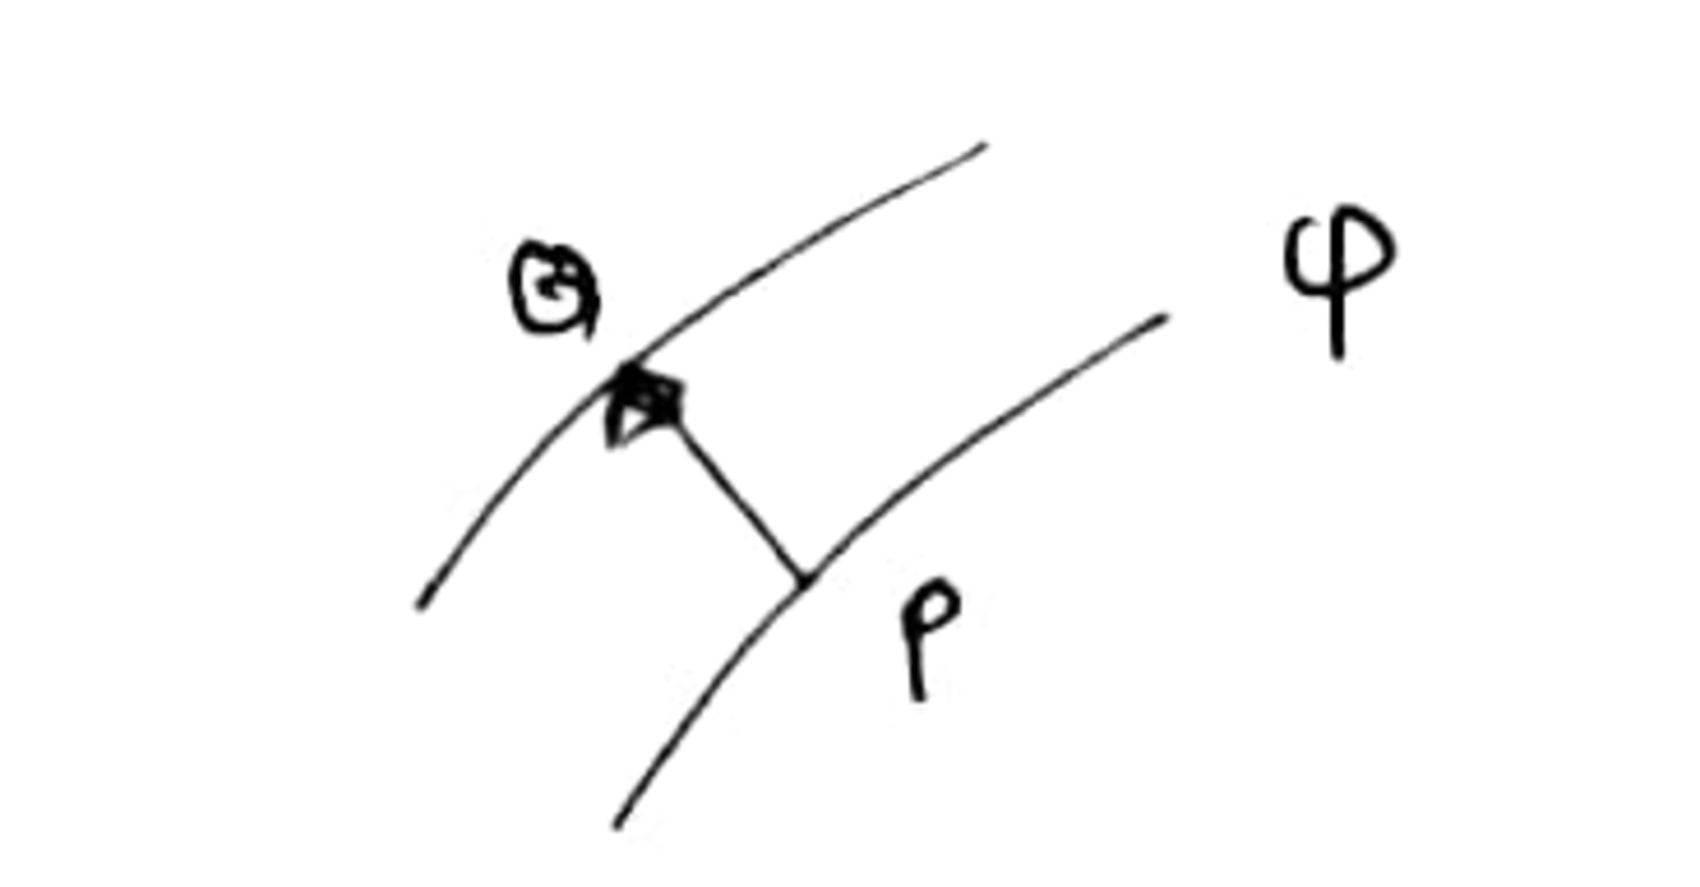
\includegraphics[width=0.3\linewidth]{figures/L2_2.jpg}
\caption*{}
\end{figure}
\vspace{-1.5cm}
\begin{align*}
    d\phi = dx\cdot \nabla \phi
\end{align*}
\begin{itemize}
    \item The gradient $\nabla \phi$ lives in the dual space.
    \item If $v \to \mathbb{R}$, and $\langle w,v \rangle \in \mathbb{R}$ then $w$ and $v$ are not in the same space.
    \item $w$ is the dual vector space of $v$.
\end{itemize}

\subsection*{Tangent Bundle}
% ----
\vspace{-1cm}
\begin{figure}[H]
\centering
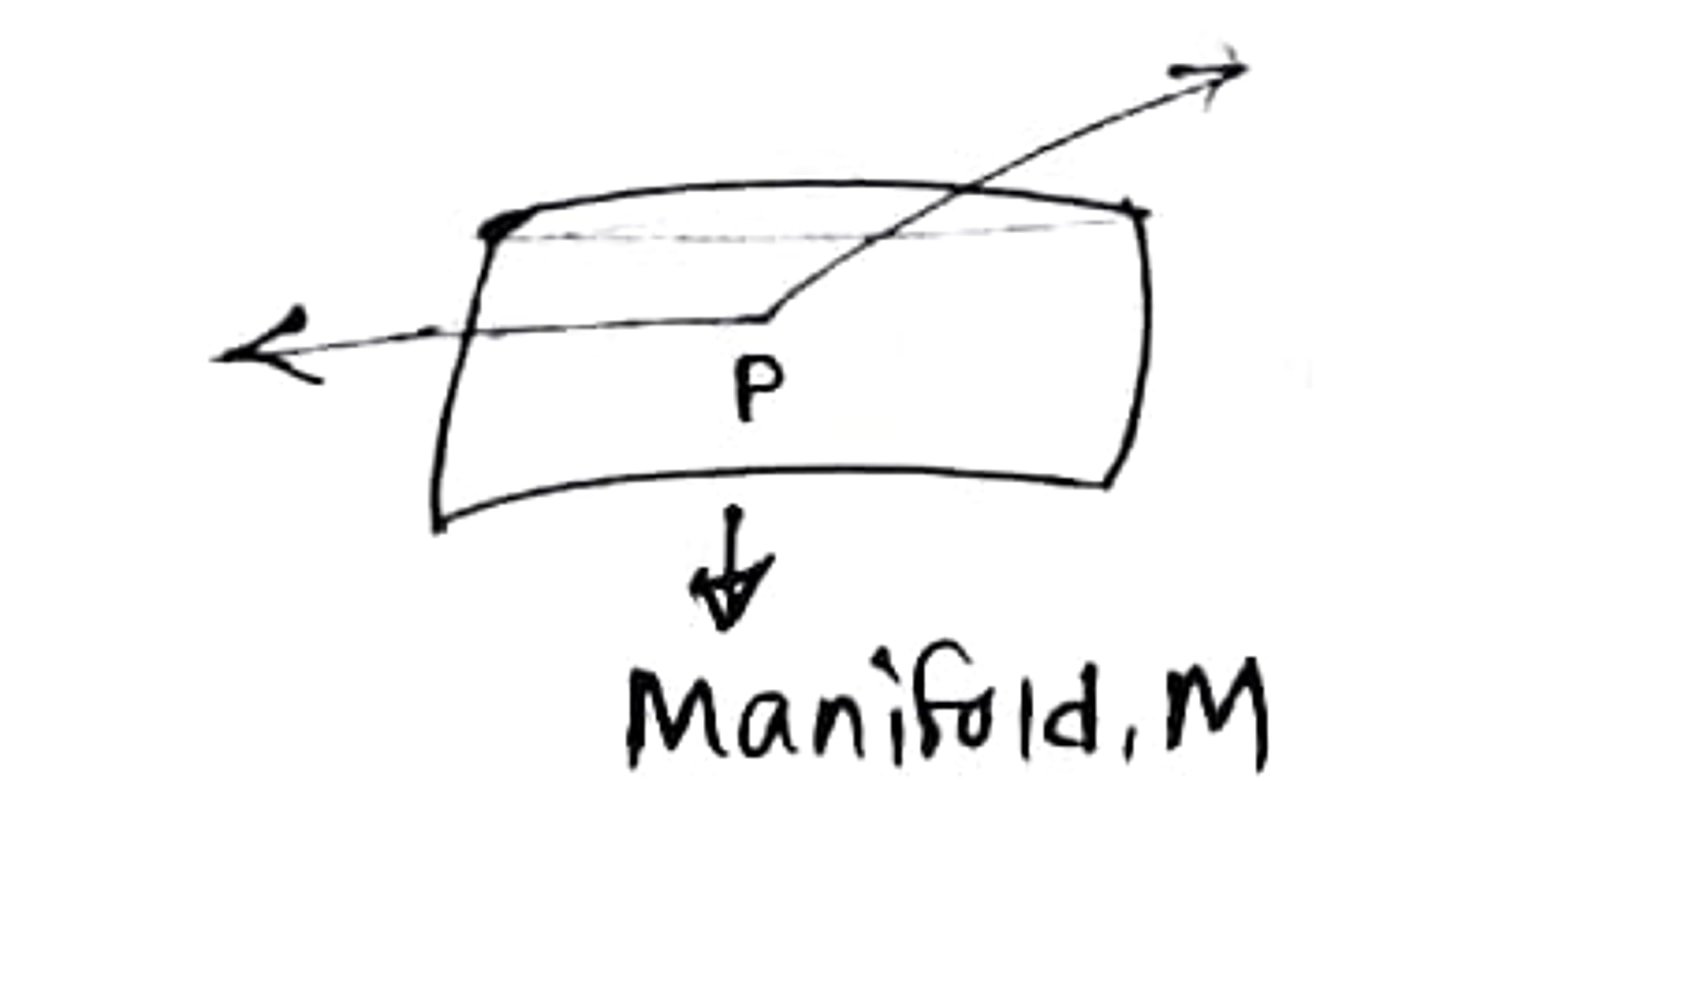
\includegraphics[width=0.45\linewidth]{figures/L2_3.jpg}
\caption*{}
\end{figure}
\vspace{-1.5cm}
A \textbf{tangent bundle} is the collection of all tangent spaces for all points on a manifold:
\begin{itemize}
    \item Let $T_p(M)$ be the tangent space at point $p$ on manifold $M$.
    \item Then, $\bigcup_p T_p(M) \equiv T(M)$ is the tangent bundle of $M$.
\end{itemize}
\begin{center}
    \fbox{\textbf{Summary}: The differential and the gradient are \textbf{dual} to each other.}
\end{center}
\subsection{Particle trajectory in a curved spacetime}
From the action:
\[
S[x] = \frac{1}{2} \int d\tau ~\dot{\xi^a}\dot{\xi^b}~ \eta_{ab}
= \frac{1}{2} \int d\tau\, G_{mn}(x) ~\dot{x}^m \dot{x}^n
\quad;\quad [\dot{x}^m \dot{x}^n =\text{squared 4-velocity term} ~]
\]
\noindent
Now, from the action principle (i.e., $\delta S = 0$), we can derive the equation of motion of the particle.
\begin{align*}
\delta S = \frac{1}{2} \int \left[ \delta G_{mn}(x)~ \frac{dx^m}{d \tau} \frac{dx^n}{d \tau} + 2 G_{mn}(x) \frac{d}{d\tau} (\delta x^m) \frac{dx^n}{d \tau} \right] d\tau
\end{align*}
Here Second term is symmetric in $m,n$, thus the term doubles. Then applying integration by parts $\left[~ u=\frac{d}{d\tau} (\delta x^m)~,~v=G_{mn}(x) \dot{x}^n=G_{mn}(x) ~\frac{dx^n}{d\tau} ~\right]$,
\begin{align*}
\delta S &= \frac{1}{2} \int \left[ \left\{\frac{\partial G_{mn}}{\partial x^p}~\dot{x}^m \dot{x}^n~\delta x^p \right\} + 2~G_{mn} \frac{dx^n}{d\tau} \delta x^m\Bigg| -2 \frac{d}{d\tau}\left(G_{mn}\frac{dx^n}{d\tau}\right)\delta x^m \right] d\tau \\
&= \frac{1}{2} \int \left[ \frac{\partial G_{mn}}{\partial x^p} \dot{x}^m \dot{x}^n~\delta x^p -2 \left(G_{mn}~\ddot{x^n}+\frac{\partial G_{mn}}{\partial x^p} \dot{x^p}\dot{x^n}  \right)\delta x^m \right] d\tau \\
&= \int \left[ \frac{1}{2}\partial_p G_{mn}~\dot{x}^m \dot{x}^n~\delta x^p - G_{mn}~\ddot{x}^n \delta x^m - \partial_p G_{mn}~\dot{x}^p \dot{x}^n~\delta x^m  \right] d\tau \\
&= -\int \left[ G_{mn}~\ddot{x^n} + \left( \partial_p G_{mn}~\dot{x^p}\dot{x^n} - \frac{1}{2}\partial_m G_{np}~\dot{x^n} \dot{x^p} \right) \right] \delta x^m~d\tau  \\
&= - \int \left[ G_{mn}~\ddot{x}^n + \frac{1}{2} \left( \partial_p G_{mn} + \partial_n G_{mp} - \partial_m G_{np} \right) \dot{x}^n \dot{x}^p \right] \delta x^m~d \tau
\end{align*}
Here, in the first line, the term $2~G_{mn} \frac{dx^n}{d\tau} \delta x^m\Bigg|=0$ at the boundary. $\delta x^\mu$ is arbitrary, therefore to satisfy the action principle, the integrand must vanish which gives:
\begin{align*}
&\quad ~~ G_{mn}~\ddot{x}^n + \frac{1}{2} \left( \partial_p G_{mn} + \partial_n G_{mp} - \partial_m G_{np} \right) \dot{x}^n \dot{x}^p = 0 \\
& \Rightarrow \ddot{x}^n + \frac{1}{2}G^{nm} \left( \partial_p G_{mn} + \partial_n G_{mp} - \partial_m G_{np} \right) \dot{x}^n \dot{x}^p = 0
\end{align*}
In the second term,
\[
\frac{1}{2}G^{nm} \left( \partial_p G_{mn} + \partial_n G_{mp} - \partial_m G_{np} \right) = \Gamma^m_{~~np} \rightarrow \text{Christoffel Symbol}
\]
\[
\boxed{\therefore \ddot{x}^n + \Gamma^m_{~~np}~ \dot{x}^n \dot{x}^p = 0}
\]
This is the \textbf{geodesic equation}.\\

\noindent
Therefore, the acceleration is proportional to the square of velocity, $\dot{x}^2$.

But in \textit{electromagnetism}:
\[
\ddot{x}^m = F^m_{~~~n}~\dot{x}^n \quad \text{(Lorentz force equation)}
\]
So here, acceleration is proportional to a 4-vector.
% ---
\begin{framed}
\noindent
\textbf{Exercise}
\[
S = \frac{1}{2} \int m~ \dot{\xi}^2 d\tau + q \int A_b(\xi) \dot{\xi}^b \, d\tau
\]
\[
\left[~\text{This latter interaction term is geometrical as well}~\right]
\]
$\bullet \quad\text{Show that we can recover the Lorentz force from here.}$
\end{framed}
% ---
\subsection{Schur's Lemma}
Schur's Lemma involves two such equations. Before understanding the lemma, we need to understand some definitions first.

\subsection*{Representation}
Let:
\[
AB = C \quad\Rightarrow \quad R(A)R(B) = R(C)
\]
Here, $R$ is a matrix-valued map that forms an algebra. This is called a \textbf{representation}.

\subsection*{Invariant Subspaces}
It begins with the question: are there subspaces on which the representation maps onto itself? The answer is \textbf{null-space} $R(0) \rightarrow 0$.
\begin{itemize}
    \item In the case of rotation, the invariant subspace is the \textbf{axis} of rotation.
    \item Except for the entire space and the trivial zero vector, any other invariant subspace (if exists) implies the representation is \textbf{reducible}.
\end{itemize}
% ---
\subsection*{Irreducible Representations (Irreps)}
If no invariant subspace exists, it is called an \textbf{irreducible representation}. For irreducible representations:
\begin{itemize}
    \item No non-trivial invariant subspaces exist.
    \item Any operator commuting with all elements of the representation is proportional to the identity.
\end{itemize}
\subsection*{Statement of Schur's Lemma}
\vspace{-0.5cm}
\begin{figure}[H]
\centering
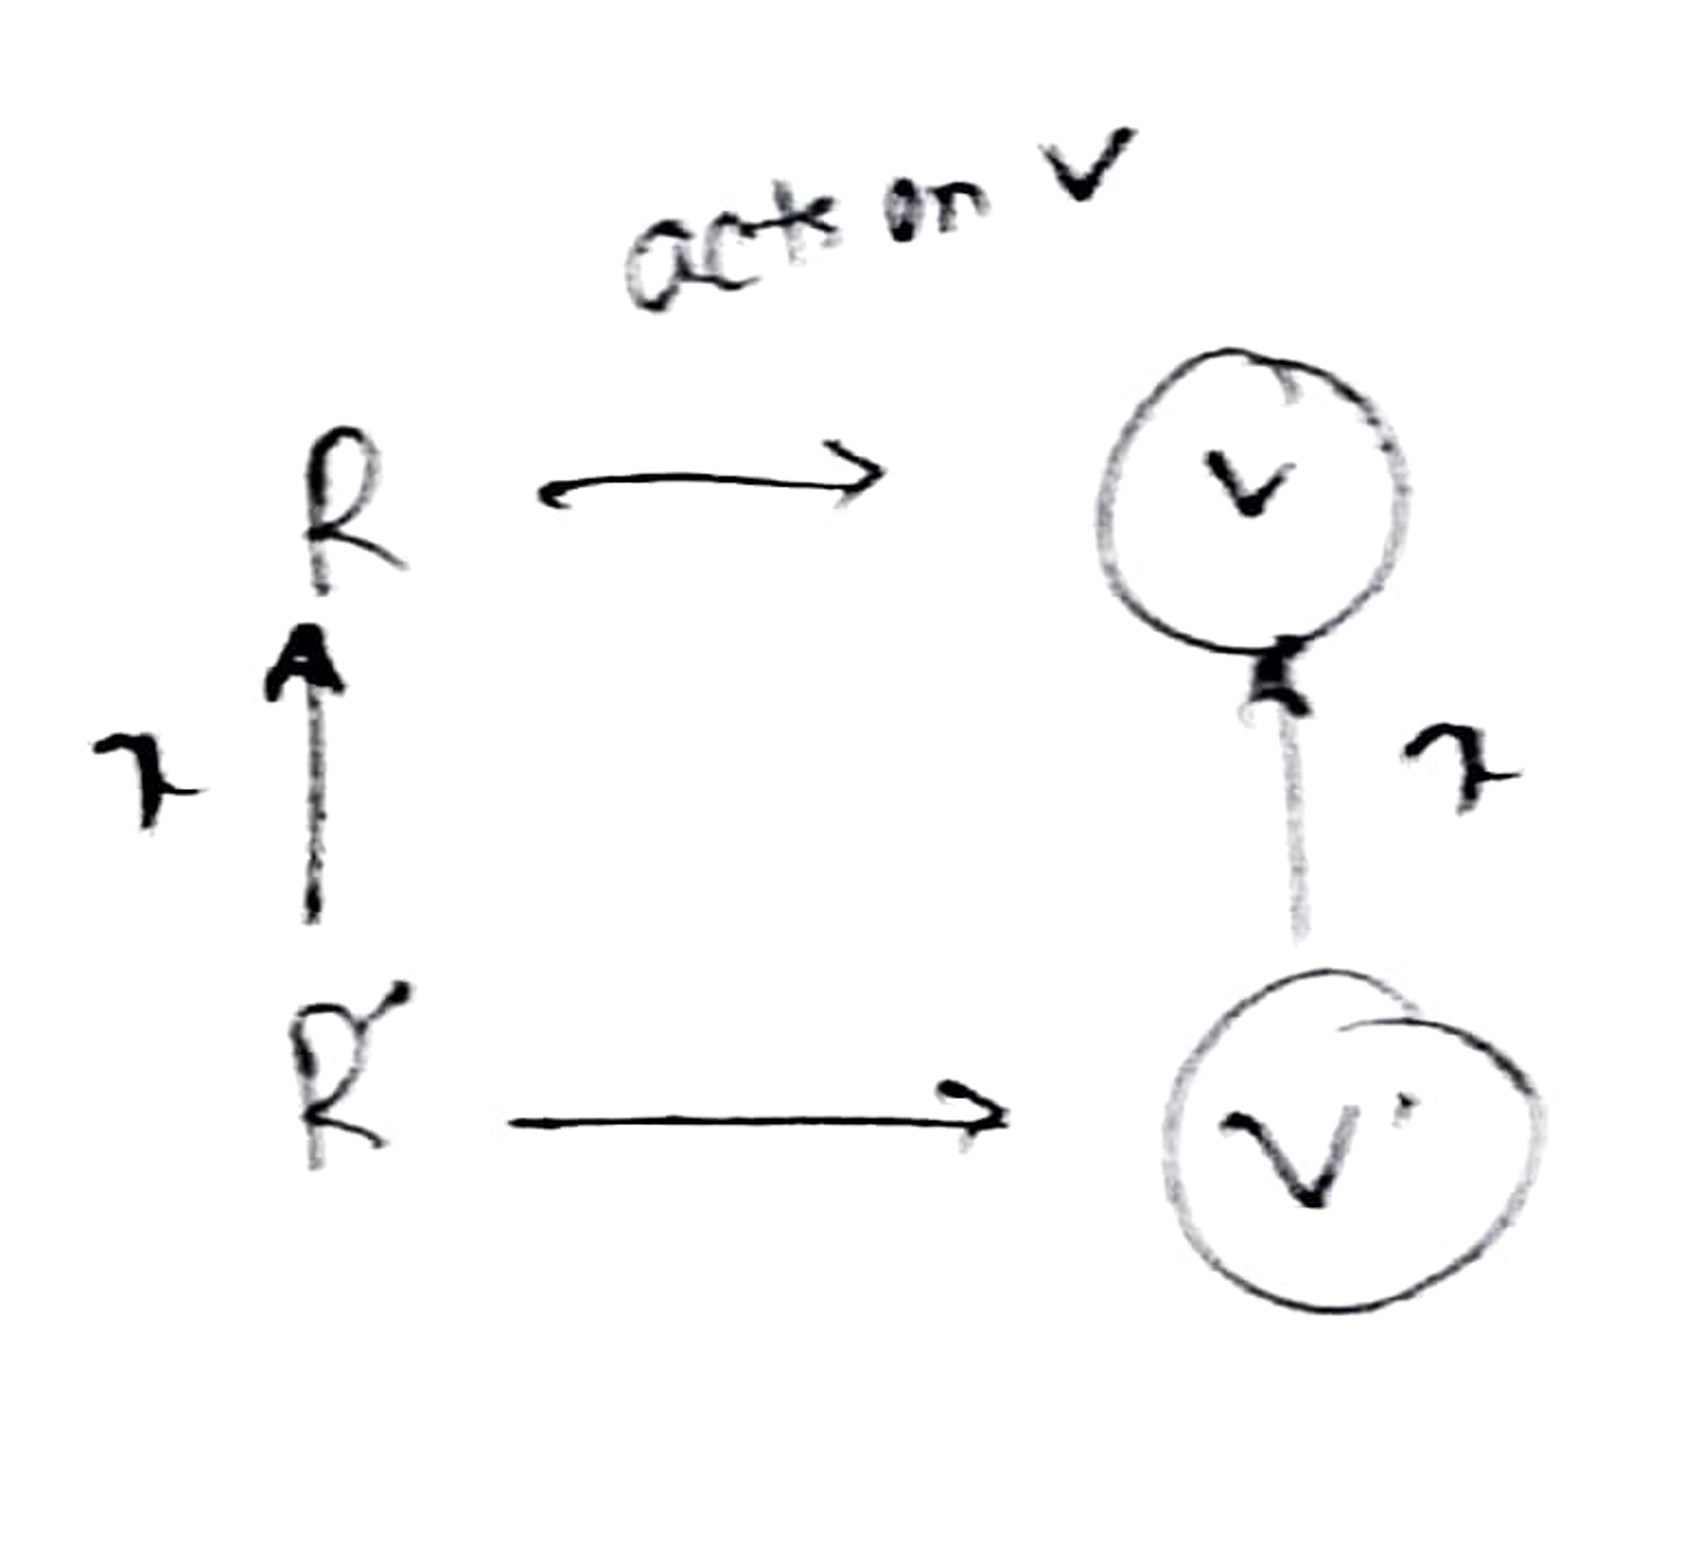
\includegraphics[width=0.3\linewidth]{figures/L2_4.jpg}
\caption*{}
\end{figure}
\vspace{-2cm}
Let $V$ and $V'$ be vector spaces, and let $R$ and $R'$ be two representations of a group $G$. That is, to each group element $g \in G$, we assign a matrix (or linear transformation) $R(g)$ acting on $V$, and $R'(g)$ acting on $V'$, such that:
\[
R(g_1 g_2) = R(g_1) R(g_2), \quad R'(g_1 g_2) = R'(g_1) R'(g_2) \quad \forall~ g_1, g_2 \in G
\]
Suppose there exists a linear map (or matrix) $X: V \to V'$ such that for all $g \in G$,
\[
X R(g) = R'(g) X
\]
\begin{tcolorbox}[ title=Intertwiner]
Let $R, R'$ be two irreps and 
$$RX = XR'$$ 
To make this possible, there exists two possibilities for $X$.
\begin{itemize}
    \item[1.] $X$ is invertible.
    \item[2.] Then: $$X^{-1} R X = R'$$
\end{itemize}
\end{tcolorbox}
\noindent
That is, $X$ \textit{intertwines} the two representations—it commutes with the group action.
If $X$ commutes with all the matrices of an irrep, then $X = \lambda \mathbb{I}$, i.e., it's proportional to the identity matrix. Example:
\[
    [J_1, J_2] = i J_3 \quad ;\quad [J^2, J_i] = 0 \quad \therefore J^2 \propto \mathbb{I}
\]
That is, any linear transformation that commutes with all the representation matrices must be a scalar multiple of the identity.
% ---
\begin{tcolorbox}[ title=Note: Commutator is a derivative]
Anything that follows the product rule, is called a \textbf{derivation}.
\begin{align*}
    \frac{d}{dx}(uv) &= \frac{du}{dx}~v ~~+~~ u~\frac{dv}{dx} \\ \\
    [A, uv] ~&= [A, u]v ~+~ u[A, v]
\end{align*}
Therefore, \textbf{Commutation} is a \textbf{derivation}
\end{tcolorbox}
% ---
\begin{framed}
\noindent
\textbf{Exercises:} Check the commutations:
\begin{align*}
    [J, p]~~ &\sim ~~p \\
    [p, p]~~ &\sim ~~0 \\
    [J, J]~~ &\sim ~J \\
    [J, p^2]~ &\sim ~0 \\
    [J, p_ap^a] &= [J, p_a]p^a + p_a[J, p^a]\sim 0
\end{align*}
Notes regarding the exercises:
\begin{itemize}
    \item We can do QFT just because of $p^2$.
    \item No quantum version of Lorentz group exists.
    \item If $[A, \mathcal{V}] = 0$, then $\mathcal
    {V}$ can only be constant.
\end{itemize}
\end{framed}
\newpage
%-------------------------------
% Section: Lecture 3
%-------------------------------
\stepcounter{section}
\renewcommand{\thesection}{\arabic{section}}
\fancysection{(\textit{\textbf{Class-6})} Lecture \textbf{3}: Sat, May 31, 2025}{\textbf{\textit{Lie Derivative}}}
%---
\subsection*{Some Clarifications from Previous Lecture}
\begin{itemize}
    \item The Lorentz group doesn't have any invariant subalgebra.
\end{itemize}
% \vspace{-0.8cm}
\textbf{Invariant Subgroup: } A subgroup $N \subset G$ is \textbf{invariant} if -
\[
g\,n\,g^{-1} \in N \quad \forall~ g \in G
\]
That means, conjugating any element of $N$ by any element of $G$ keeps it inside $N$. Therefore, for any group element $g$, if
\begin{align*}
& g\,g^{-1} = g''\quad \text{(conjugating each like similarity transformation)} \\
\Rightarrow h g h^{-1} &\cdot h g h^{-1} = h\,g''\,h^{-1}~~(\text{where } hgh^{-1} = g, \; h \in G )\\
\Rightarrow &g\,g^{-1} = g\,g^{-1} \quad \therefore \quad h\,e\,h^{-1} = e \rightarrow \text{unaffected}
\end{align*}
\subsection*{Invariant} 
\vspace{-1cm}
\begin{figure}[H]
\centering
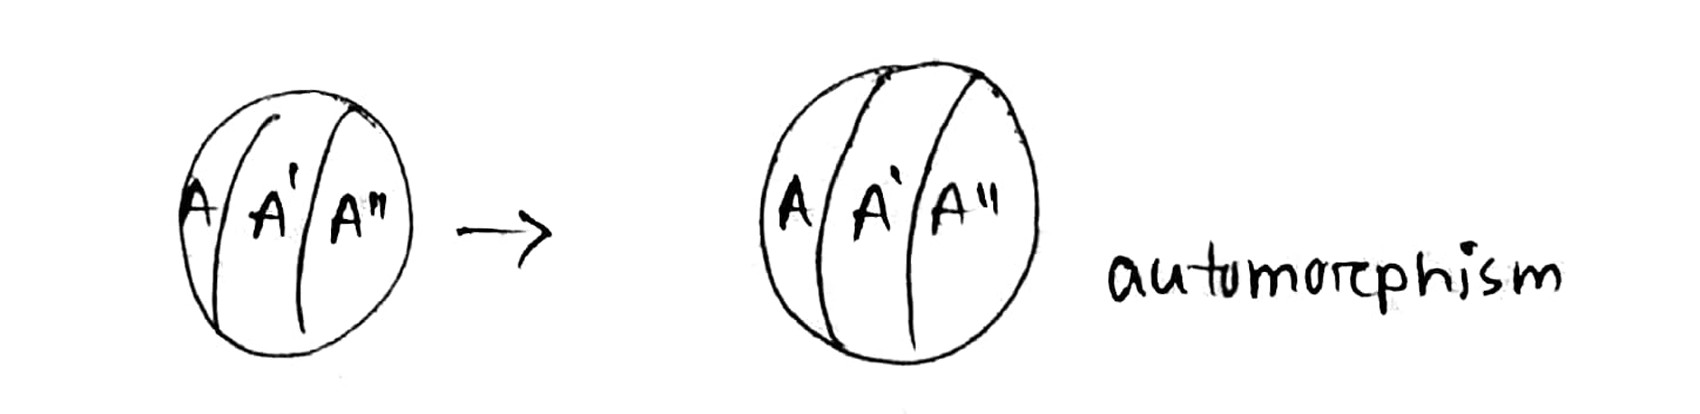
\includegraphics[width=0.7\linewidth]{L3_1.jpg}
\caption*{}
\end{figure}
\vspace{-1cm}
\noindent
Under conjugation, things get mapped, but some things remain unchanged — that is called \textbf{invariant}.

\subsection*{Automorphism}
An \textbf{automorphism} is a structure-preserving map from a mathematical object to itself.

\subsection*{Invariant Subalgebra}
A subalgebra $h \subset g$ is said to be \textbf{invariant} if:
\[
[X,H] \in h \quad \forall~ X \in g, \, H \in h
\]
That is, the Lie bracket of any element of the full algebra with any element of the subalgebra lies inside the subalgebra.\\
Therefore, if $h = e^A$ where $A \in$ Lie algebra and $h \in$ Lie group, then:
\begin{align*}
&h\,g\,h^{-1} = g' \\
\Rightarrow e^A e^B e^{-A} &\sim e^{B+[A,B]} = e^{B'} \quad (\because [A,B] \sim B' )
\end{align*}
\begin{center}
    ($g$ doesn’t have to be $g'$, it just has to map into the subalgebra.)
\end{center}
Because boosts and rotations are mixed under commutators, they don’t form invariant pieces.
% ---
\begin{tcolorbox}[ title=Notes]
\begin{itemize}
    \item The Lorentz group also has no unitary representation because it is \textbf{non-compact}.
    \item The Poincare group has unitary representation because is \textbf{compact}.
    \item Every finite group has a unitary representation.
    \item \textbf{Peter-Weyl theorem} states that “compact groups have the same structure as finite groups.”
    \item Hence, compact groups too have a unitary representation.
    \item On the other hand, boost transformations form an infinite set of elements.
    \item Boosts are parameterized by the \textit{rapidity} (or velocity), which is a continuous real parameter.
    \item Boosts are generated by the non-compact part of the Lorentz algebra $SO(1,3)$.
    \item Since the group is continuous and non-compact, it has infinitely many elements—like translations or rotations. Hence, \textbf{no unitary representation}.
\end{itemize}
\end{tcolorbox}
% ---
% \subsection*{Induced Representation}

\subsection{Lie Derivative}

\subsubsection{Congruence}
A congruence is a family of smooth curves such that through every point in a region (or patch) of spacetime, exactly one curve passes.

\begin{itemize}
    \item Congruence implies a well-defined vector field and vice-versa.
    \item \textit{Diffeomorphism:} A map from spacetime into itself in a continuous manner, again in the same space.
\end{itemize}
\vspace{-0.5cm}
\begin{figure}[H]
\centering
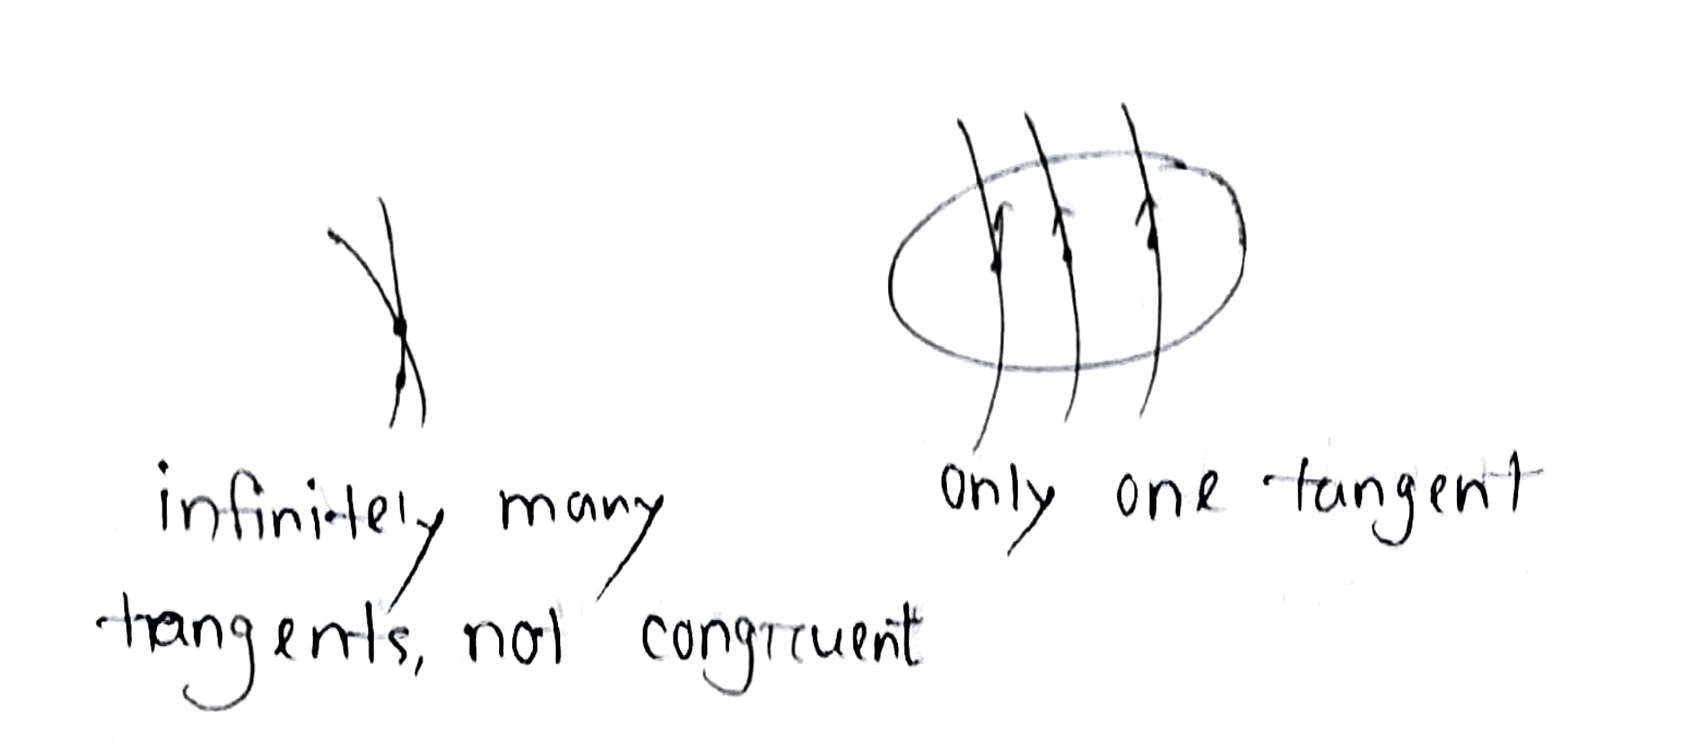
\includegraphics[width=0.7\linewidth]{figures/L3_2.jpg}
\caption*{}
\end{figure}
\vspace{-1cm}
\noindent 
\subsubsection*{Defining Lie Derivative}
We have learned about congruence because $-$``The Lie derivative measures how a tensor field changes along a flow, and a congruence provides exactly that flow.''

\begin{itemize}
    \item Lie derivative only needs congruence/vector field.
    \item Covariant derivative needs dot product (metric structure).
\end{itemize}
% \vspace{-1cm}
\begin{figure}[H]
\centering
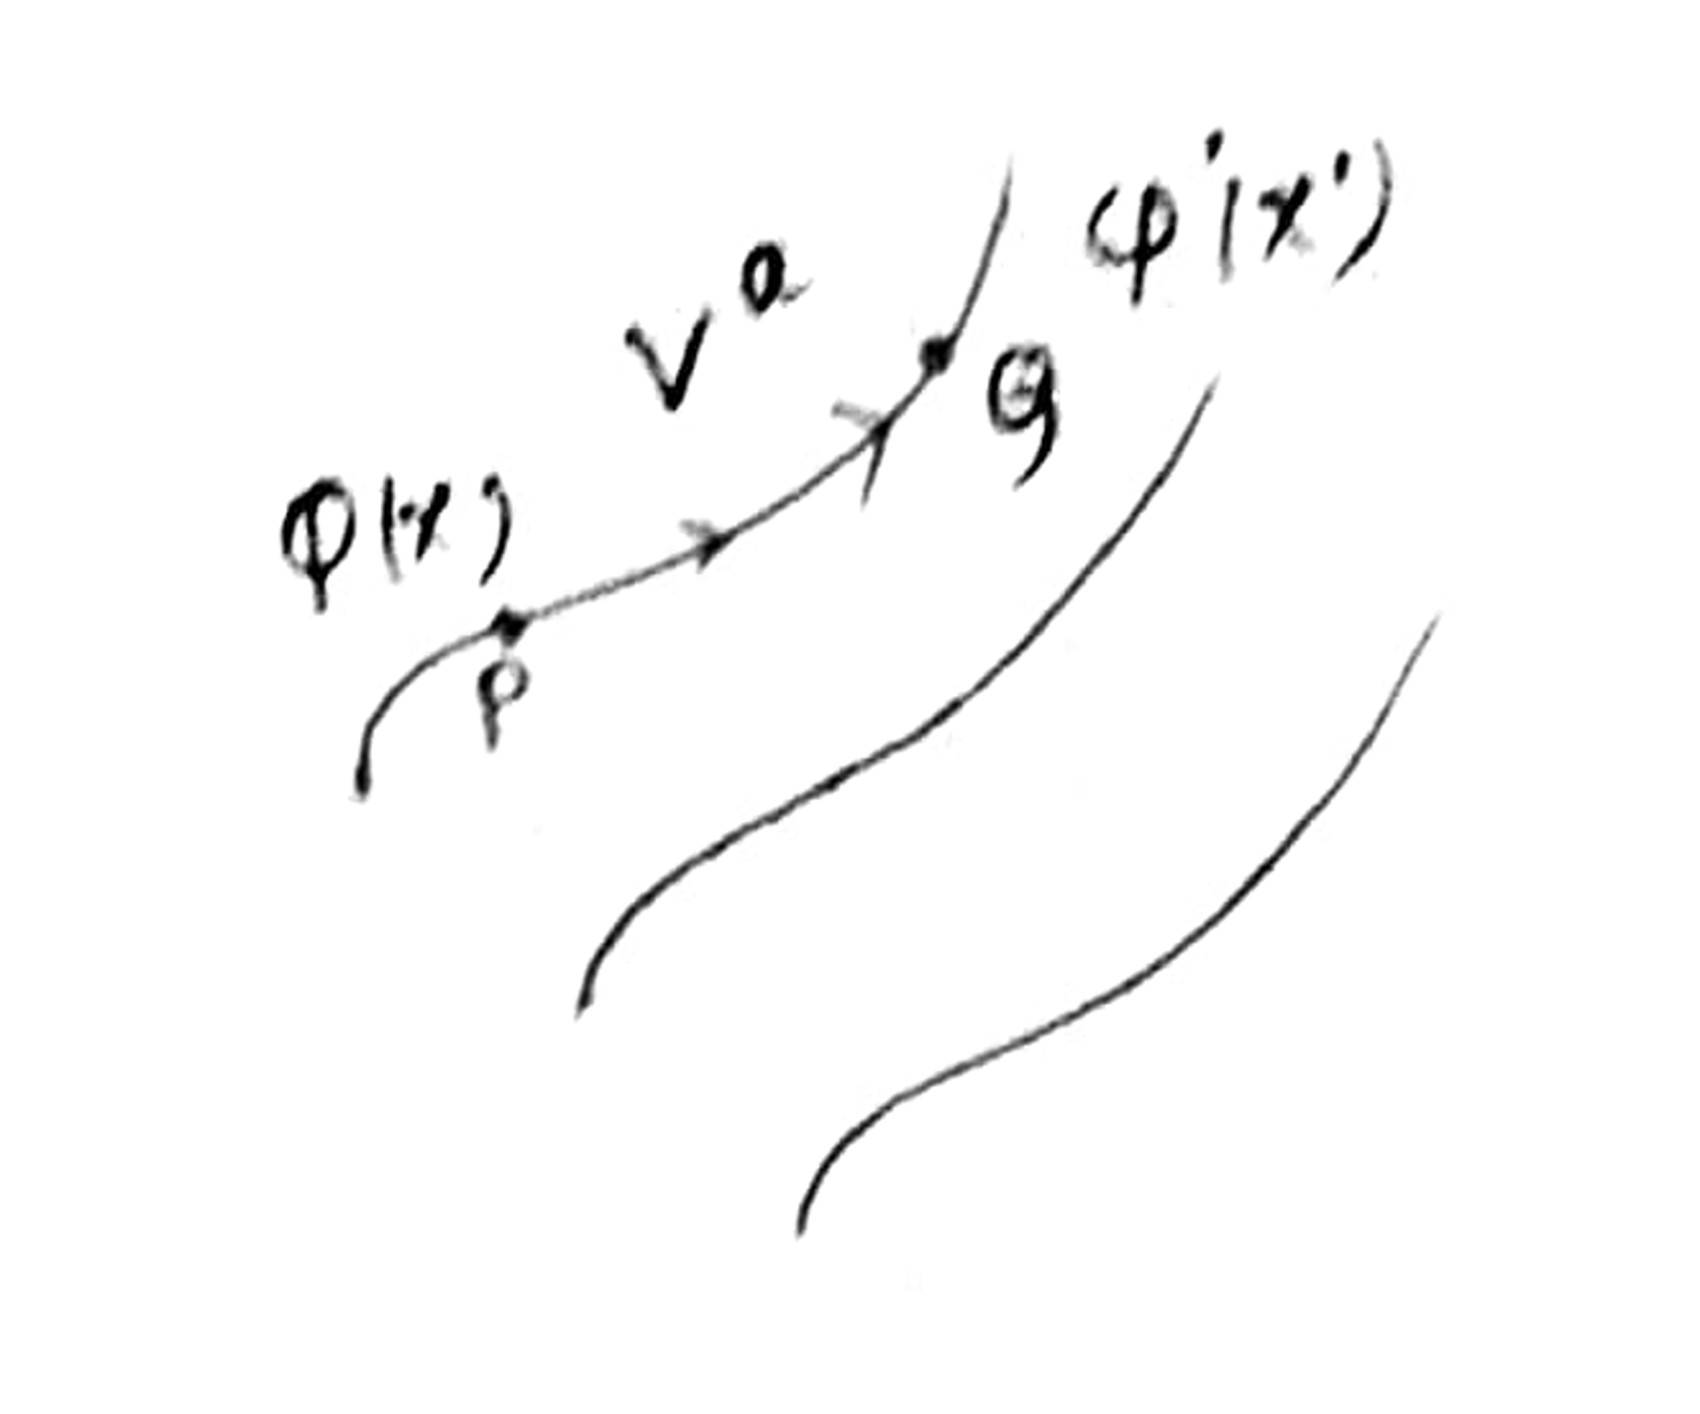
\includegraphics[width=0.3\linewidth]{L3_3.jpg}
\caption*{}
\end{figure}
\vspace{-1cm}
Let point $P$ be mapped into $Q$ due to congruence. Let the coordinate transformation be:
\[
x^a \rightarrow x'^a = x^a + t \,v^a,
\]
\begin{itemize}
    \item It is a flow where $t$ is a flow parameter (an infinitesimal step)
    \item $v^a$ is the vector field generating the flow.
\end{itemize}
Therefore, the Lie derivative of a scalar field $\phi$ is defined as:
\[
\boxed{\mathfrak{L}_v \phi = \lim_{t \to 0} \frac{\phi_{-t}(x') - \phi(x)}{t}}
\]
\noindent This describes the evolution of the field along the flow lines defined by the congruence.
% ---
\begin{tcolorbox}[proofbox, title=Note: Why $\phi_{-t}(x')~?$]
The evolution of the system itself. Negative time means back to its own position.
% \vspace{-0.5cm}
\begin{figure}[H]
\centering
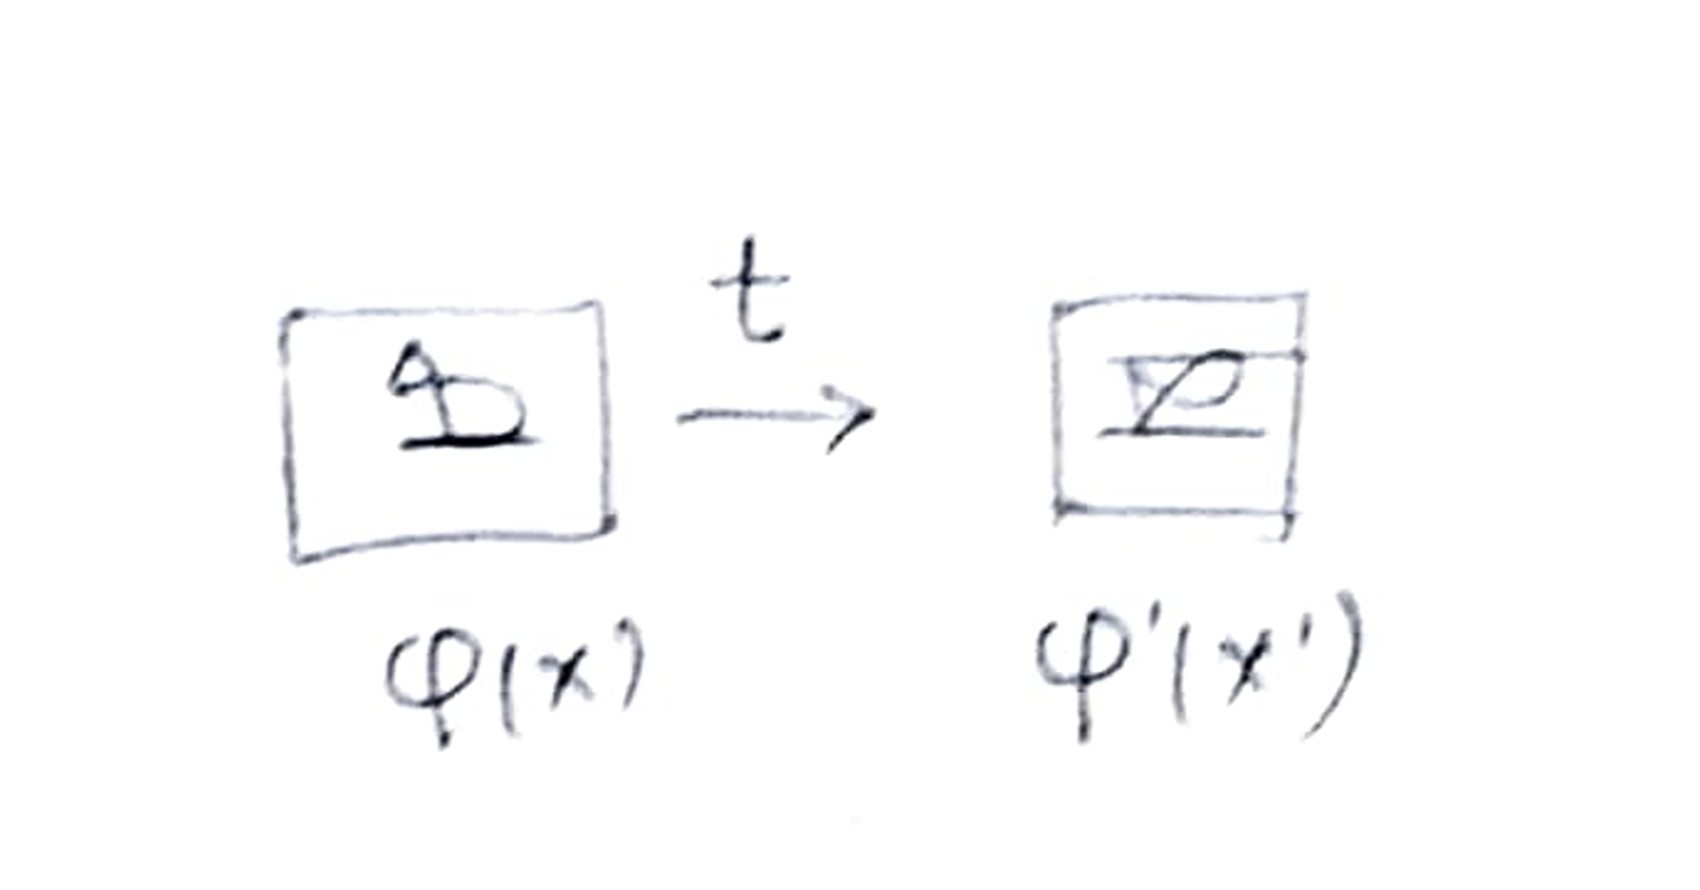
\includegraphics[width=0.35\linewidth]{L3_4.jpg}
\caption*{}
\end{figure}
\vspace{-1cm}
\end{tcolorbox}
% ---
\subsection{Lie Derivative for a Scalar Field}
\vspace{-0.5cm}
\begin{figure}[H]
\centering
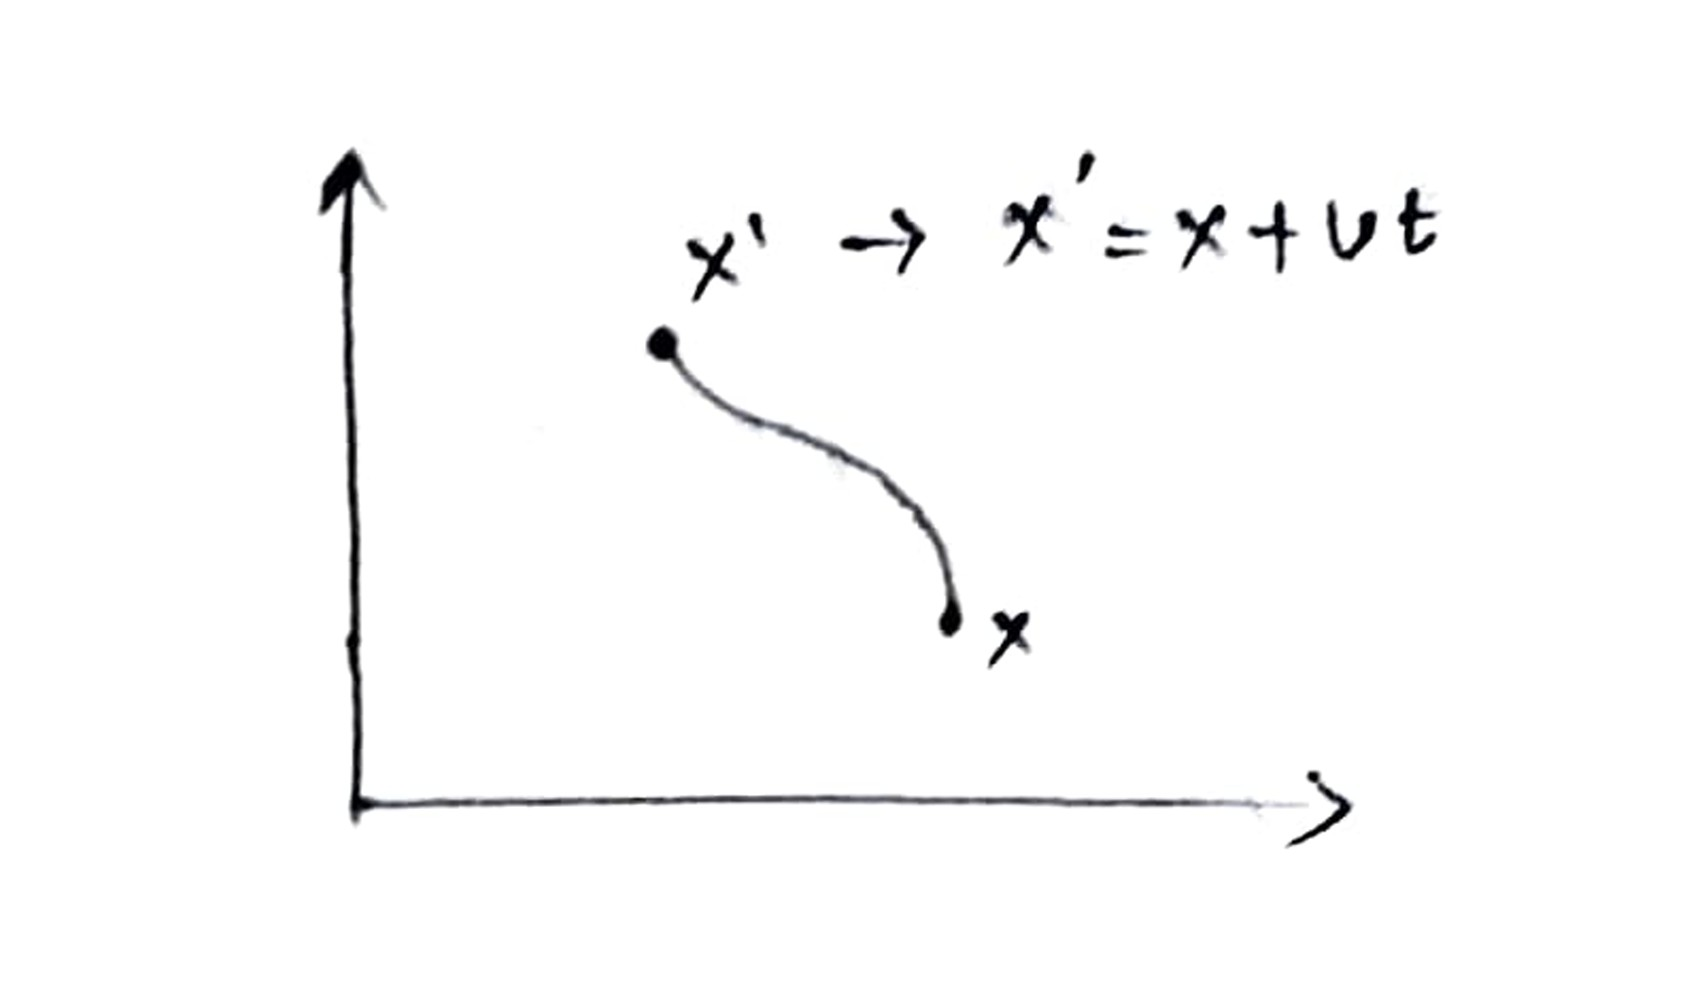
\includegraphics[width=0.4\linewidth]{L3_5.jpg}
\caption*{}
\end{figure}
\vspace{-1cm}
Here, only coordinates change, the field doesn't change. Therefore, for a scalar field, it is simply, $\phi'(x') = \phi(x)$, no involvement of direction. We want to calculate the field at the initial position, i.e.,
\begin{align*}
\phi'(x) &= \phi'(x' - vt) \\
&= \phi'(x') - t\, v^a \partial_{a} '\, \phi'(x') + \dots \quad  [\text{Expanding in Taylor series}] \\
&= \phi(x) - t\, v^a \partial_a'\, \phi(x) \quad \quad [\text{Only keeping the first-order term in $t$}]
\end{align*}
Therefore, the Lie derivative:
\begin{align*}
\mathfrak{L}_v \phi &= \lim_{t \to 0} \frac{\phi'(x) - \phi(x)}{t} \\
&= \lim_{t \to 0} \frac{- t \,v^a\, \partial_a \phi(x)}{t} \\
&= -v^a \partial_a \phi(x) \\
&= - (\vec{v} \cdot \nabla) \phi(x) \\
&= - \hat{v}~ \phi(x)
\end{align*}
This is nothing but the directional derivative in $3D$.

Hence, the Lie derivative of a scalar field is just the directional derivative of $\phi$ along the vector $v^a$. And it's a linear combination of partial derivatives weighted by the components of the vector field $v^a$.

\subsection{Lie Derivative of a Vector Field}
Similarly, $V(x)$ is a vector field defining the flow, and $W(x)$ is another vector field (the one we want to differentiate). Now, the lie derivative:
\[
\mathfrak{L}_{\hat{V}} W^a = \lim_{t \to 0} \frac{W'\,^b(x) - W^a(x)}{t}
\]
\[
\text{(where $W'\,^b$ is the new vector field at position $Q$, while $W^a$ is at position $P$)}
\]
This change tells us how the vector field $W$ changes when dragged along the flow generated by $V$. Therefore,
\begin{align*}
& \quad \quad x \quad \rightarrow \quad x' + Vt \\
& \quad ~~W^a(x) \rightarrow W'\,^b(x') = \frac{\partial x'^a}{\partial x^m} W^m(x) \\\\
& \Rightarrow W'\,^b(x') = \frac{\partial}{\partial x^m}(x^a + V^a t)~W^m(x) \\\\
& \Rightarrow W'\,^b(x + Vt) = \left( \delta^a_m + t\,\partial_m V^a \right)~W^m(x) \\\\
& \Rightarrow W'\,^b(x)+ t\,V^b \partial'_b\,W^b(x) = \delta^a_m\,W^m(x) + t W^m(x) \partial_m V^a \\\\
& \Rightarrow W'\,^b(x) - W^a(x) = t \left(W^m~\partial_m V^a - V^b~ \partial'_b ~W'\,^b \right) \\\\
& \Rightarrow \frac{W'\,^b(x) - W^a(x)}{t} = W^m~\partial_m V^a - V^b~ \partial'_b ~W'\,^b \\\\
&  \boxed{\therefore \mathfrak{L}_{\hat{V}} W^a = W^m~\partial_m V^a - V^b~ \partial'_b ~W'\,^b = W^m~\partial_m V^a - V^b~ \partial_b ~W^a}
\end{align*}
This is the lie derivative of a vector field. Let's simply it,
\begin{align*}
(\mathfrak{L}_{\hat{V}} W^a)(\phi) & = (W^m~\partial_m V^a - V^b~ \partial_b ~W^a)\phi= (W^b~\partial_b V^a - V^b~ \partial_b ~W^a) \phi \quad[m=b] \\\\
& = (W^b~\partial_b V^c - V^b~ \partial_b ~W^c) \partial_c \phi \\\\
&= (W^b~\partial_b V^c ~\partial_c \phi + W^b V^c~\partial_b \partial_c \phi) - (V^b~ \partial_b ~W^c~\partial_c \phi + W^b V^c~\partial_b \partial_c \phi) \\\\
&= W^b \partial_b (V^c ~ \partial_c \phi) - V^b \partial_b (W^c ~ \partial_c \phi) \\\\
& = ( \hat{W} \hat{V} - \hat{V} \hat{W})\, \phi(x) \\\\
& =[ \hat{W}, \hat{V} ]\, \phi(x) = -[ \hat{V}, \hat{W} ]\, \phi(x)\\\\
& \boxed{\therefore \mathfrak{L}_{\hat{V}} W^a = -[\hat{V}, \hat{W}]^a}
\end{align*}
Hence, two vector fields are mapped to another vector field. 
$[ \hat{V}, \hat{W}]$ creates a vector field out of the two vector fields $\hat{V}$ and $\hat{W}$.
% ---
\begin{tcolorbox}[ title=Note:]
Recall the Jacobi identity:
\[
\left[~ [ A, B], C~ \right] + \left[ ~[ B, C], A~ \right] + \left[~[ C, A ], B~ \right] = 0
\]
\begin{center}
    \textbf{The Jacobi identity is true for all algebra.}
\end{center}
\end{tcolorbox}
% ---
\begin{framed}
\noindent
\textbf{Exercise:}\quad Show that-
\[
\mathfrak{L}_{\hat{V}} \mathfrak{L}_{\hat{W}} - \mathfrak{L}_{\hat{W}} \mathfrak{L}_{\hat{V}} = \mathfrak{L}_{[\hat{V},\hat{W}]}
\]
\end{framed}
SO far we've seen that a Lie derivative maps -
\begin{itemize}
    \item Scalar to scalar
    \item Vector to vector
    \item Tensor to tensor. All of the same type.
\end{itemize}
% ---
\begin{tcolorbox}[ title=Covector]
A \textbf{covector} is a type of linear map that acts on vectors and returns real or complex numbers.
\begin{itemize}
    \item A vector is an element of the space V
    \item A covector is an element of the dual space $V^*$
\end{itemize}
\[
\text{(Vector)}^b \cdot \text{(Covector)}_b = \text{Scalar}
\]
\end{tcolorbox}
% ---
\subsection{Lie Derivative of a Covector}
\begin{align*}
&\quad \quad \mathfrak{L}_{\hat{V}} (W^a U_a) \quad = \quad - ~V^c \partial_c (W^a U_a) \\\\
&\Rightarrow (\mathfrak{L}_{\hat{V}} W^a) U_a + W^a (\mathfrak{L}_{\hat{V}} U_a) = - \{~V^c (\partial_c W^a)U_a + V^c W^a~ (\partial_c U_a)~\} \\\\
&\Rightarrow (W^c~ \partial_c V^a - V^c~ \partial_c W^a) U_a + W^a (\mathfrak{L}_{\hat{V}} U_a) = -~V^c (\partial_c W^a)U_a - V^c W^a~ (\partial_c U_a) \\\\
& \Rightarrow W^c~ \partial_c V^a ~U_a + W^a (\mathfrak{L}_{\hat{V}} U_a) = - V^c W^a~\partial_c U_a \\\\
& \Rightarrow W^a (\mathfrak{L}_{\hat{V}} U_a) = - (W^c~ \partial_c V^a ~U_a+V^c W^a~\partial_c U_a) \\\\
& \Rightarrow W^a (\mathfrak{L}_{\hat{V}} U_a) = - (W^a~ \partial_a V^c ~U_c+V^c W^a~\partial_c U_a) = -~W^a~(\partial_a V^c ~U_c+V^c~\partial_c U_a)
\end{align*}
\[
\boxed{\therefore \mathfrak{L}_{\hat{V}} U_a = -(V^c~\partial_c U_a + \partial_a V^c ~U_c)}
\]
\newpage

\stepcounter{section}
\renewcommand{\thesection}{\arabic{section}}
\fancysection{(\textit{\textbf{Class-7})} Lecture \textbf{4}: Wed, June 18, 2025}{\textbf{\textit{Covariant Derivative}}}
%---
\subsection*{Deriving Lie Derivative from the Vector Field}
\vspace{-0.7cm}
\begin{figure}[H]
\centering
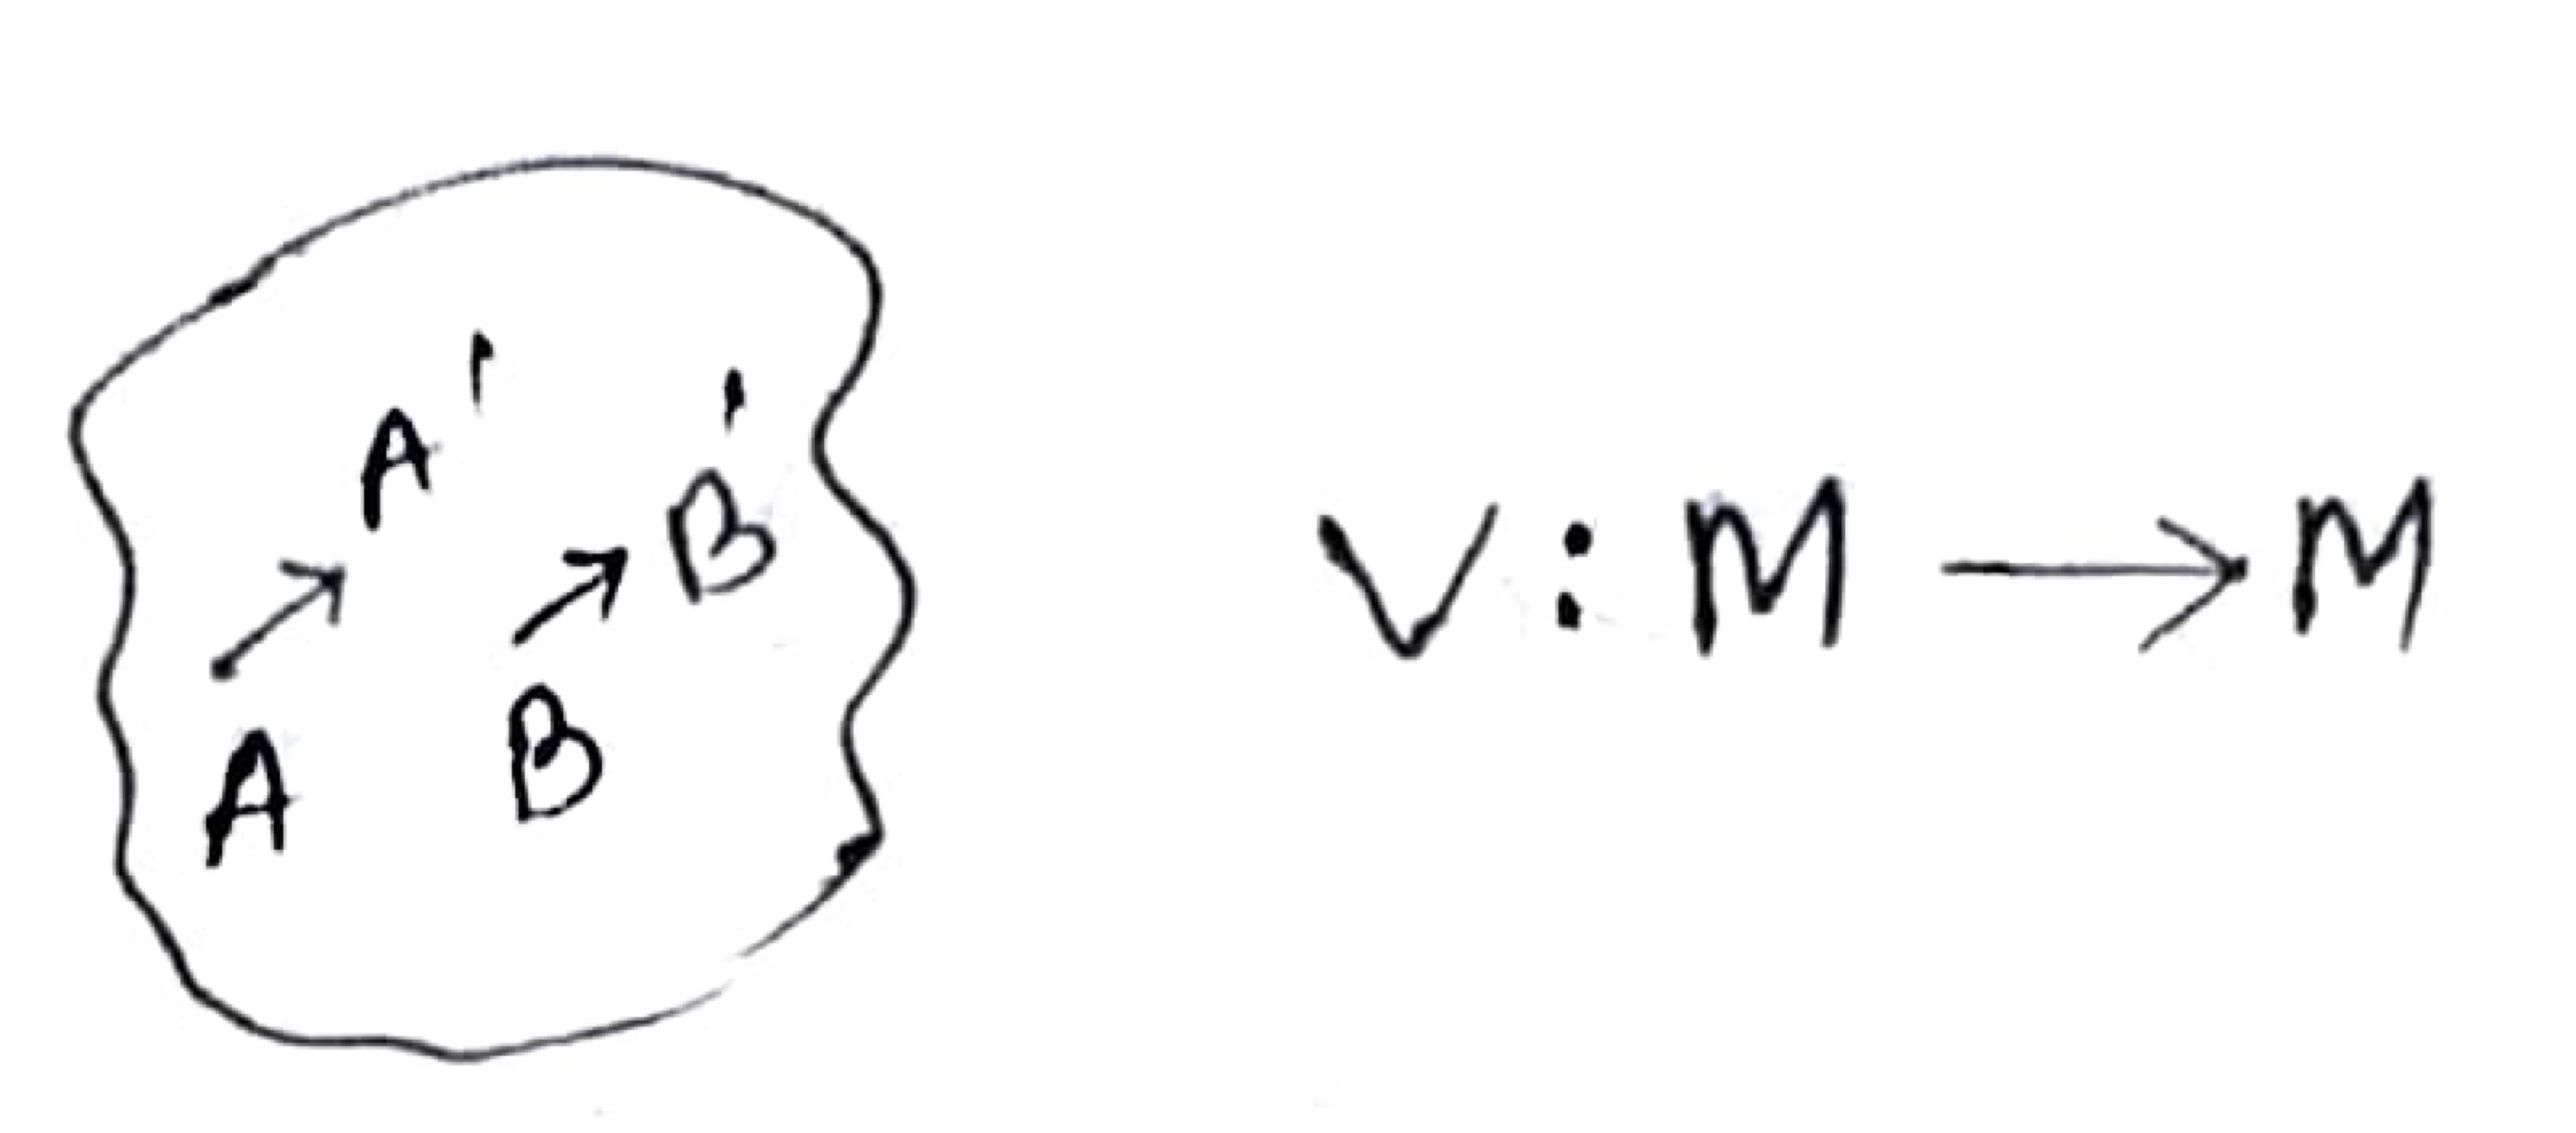
\includegraphics[width=0.4\linewidth]{L4.jpeg}
\caption*{}
\end{figure}
\vspace{-1cm}
\begin{itemize}
\item Vector field maps from manifold to manifold.
\item All Lie groups are manifolds, but all manifolds are not Lie groups.
\item Lie derivative can be defined on any manifold.
\item In a manifold, there is no composition rule.
\end{itemize}
\begin{tcolorbox}[ title=Previous class discussion]
$\bullet$ Adjoint map and Lie derivative are not same.

Adjoint definition :
\[
\langle v,A \rangle = \langle A^*v , u \rangle
\]
Whereas, Lie derivative:
\[ \mathfrak{L}_v \, u = -[u,v] = [v,u] \]

$\bullet$ Lie derivative and Lie algebra are not same.
\[
f=f(x,y) \quad; \quad g=g(x,y)
\]
\begin{align*}
f=f(x,y) \quad; \quad g=g(x,y) \\
v = f \frac{\partial}{\partial x} + g \frac{\partial}{\partial y} \\
[v,v'] = \frac{\partial f}{\partial x}\frac{\partial g}{\partial y} - \frac{\partial g}{\partial x} \frac{\partial f}{\partial y} \tag{7.1} \label{7.1}
\end{align*}
This \eqref{7.1} is not constant for Lie derivative. However,
\[
[T^a , T^b] = f^{ab}\,_c \,T^c \tag{7.2} \label{7.2}
\]
The term $f^{ab}\,_c$ in \eqref{7.2} is \textbf{constant} in Lie algebra or Lie group.
\end{tcolorbox}
% ---
Now, $\xi^a =$ local cartesian coordinate. We know that,
\[
ds^2 = \left( d \xi^a \right)^2 = \delta_{ab}~d\xi^a d\xi^b \tag{7.3} \label{7.3}
\]
But we also know that,
\begin{align*}
d\xi^a &= \frac{\partial\xi^a}{\partial x}dx^m \tag{7.4} \label{7.4} \\
\Rightarrow d\xi^a&= M^a\,_m ~dx^m \\
\therefore~ dx^m &= (M^{-1})^m{}_a \, d\xi^a
\end{align*}
\textbf{Notes :}
\begin{itemize}
\item A vector has to transform according to \eqref{7.4}.
\item If $M^{-1}$ doesn't exist, we can onlyy go to one way, known as singular. Example - the origin.
\end{itemize}
Using \eqref{7.4} to \eqref{7.3} we get
\begin{align*}
ds^2 &= \delta_{ab} \frac{\partial\xi^a}{\partial x^m} \frac{\partial  \xi^b}{\partial x^n}~dx^m \, dx^n \\
\therefore~ ds^2 &= G_{mn} \, dx^m \, dx^n \quad ; \quad G_{mn} = G_{nm} \quad \text{(symmetric)}
\end{align*}
If such symmetric $G_{mn}$ exists which is also invertible, the manifold is called \textbf{Riemannian manifold}.

Since $ds^2$ is a scalar, it can also be given as:
\[
    \langle v, u \rangle \equiv g_{ab} \, V^a \, V^b
\]

\subsection{Killing Vector}
[It is connected to symmetry hence related to a conserved quantity via Noether's theorem.]\\

\noindent
\textbf{Definition:} A vector field $X$ on $M$ is called a Killing vector field if the Lie derivative of the metric with respect to $X$ is zero:
\[
    \mathfrak{L}_X~g_{ab} = 0
\]
\noindent
This means that the metric doesn't change along the flow of $X$, i.e., distances and angles are preserved under the transformation generated by $X$.
\begin{tcolorbox}[ title=Cyclic Coordinates]
A cyclic coordinate is a generalized coordinate $q_i$ that doesn't appear explicitly in the Lagrangian $\mathcal{L}(q, \dot{q},t)$. 
\[
    \frac{\partial \mathcal{L}}{\partial q_i} = 0
\]
Which implies $q_i$ is cyclic.

\end{tcolorbox}
Also,
\[
    [\mathfrak{L}_u, \mathfrak{L}_v] = \mathfrak{L}_{[u, v]}
\]
Two Killing vectors also constitute another Killing vector.
\subsection{Covariant Derivative}

\begin{itemize}
    \item[1.] It has to satisfy Leibniz rule (Derivative).
    \item[2.] Mapping from algebra to algebra.
\end{itemize}
Now, $D : A \rightarrow A$
\begin{align*}
D(ab) = (Da)b + a(Db) \quad; \quad a, b \in A \\
\end{align*}
For a constant $c$,
\[
D(ca) = (Dc)a + c(Da) = c(Da)
\]
\[
    \therefore (Dc) \text{ needs to be zero for a constant } c
\]

Also,
\[
    D g_{ab} = 0 \quad \Rightarrow \quad \nabla_m~ g_{ab} = 0
\]

\begin{itemize}
    \item $\nabla \rightarrow$ generic case
    \item $\partial \rightarrow$ flat space only
\end{itemize}

When $\nabla_a$ hits a scalar $\phi$, it produces a vector:
\[
    \nabla_a \phi = \partial_a \phi \quad \text{(vector)}
\]
But,
\[
    \nabla_a u^b \ne \partial_a u^b \quad \text{in this way.}
\]
Like,
\begin{align*}
& U^b \rightarrow U'^c = M^c{}_b \, U^b \\
\Rightarrow ~& \partial_d'~U'^c = \partial_d' (M^c{}_b \, U^b) \\
\Rightarrow ~& \partial'_d~U'^c = M^c\,_b \,\partial'_d \,U^b + (\partial'_d M^c{}_b)\, U^b
\end{align*}
Here exist an additive part, $(\partial'_d M^c{}_b)\, U^b$ that is the problem part which keeps the traces of previous map, mixing of objects of different type. Therefore, to kill it, we need to get:
\[
\partial'_d\,M^c{}_b = 0.
\]
Hence,
\[
\nabla'_a (M U) = M \,\nabla_a U \quad \text{and} \quad \nabla'_a \rightarrow M^{-1} \nabla_a \, M.
\]
Now,
\[
\nabla_a = \partial_a + A_b
\]
This $A_b$ is the additive part called the connection. In older books it was called \textbf{connexion}.

Also,
\begin{align*}
& \nabla_a \phi = \partial_a \phi \\
\Rightarrow~ &\nabla_a U^b = \partial_a U^b + {\Gamma_a\,^b}_{c}\, U^c \tag{7.5} \label{7.5} \\
\Rightarrow~ & \nabla_a V_b = \partial_a V_b - \Gamma_{ab}^c V_c
\end{align*}
The connection in \eqref{7.5} is called \textit{Levi-Civita connection}. Now let,
\begin{align*}
& U^a \nabla_a = \phi \\
\Rightarrow~ & \nabla_c (U^a \nabla_a) = \partial_c \phi \\
\Rightarrow~ & (\nabla_c U^a)\nabla_a + U^a (\nabla_c \nabla_a) = \partial_c \phi
\end{align*}
Then,
\begin{align*}
\nabla_a (V_b\,W_c) &= (\nabla_a V_b) W_c + V_b (\nabla_a W_c) \\
&= \partial_a (V_b W_c) - \Gamma^d_{ab} V_d W_c - \Gamma^d_{ac} V_b W_d \\
\therefore \nabla_a~g_{bc} &= \partial_a\,g_{bc} - \Gamma^d_{ab}~g_{dc} - \Gamma^d_{ac}~g_{bd} 
\end{align*}
Previously, we know that:
\begin{align*}
\mathfrak{L}_V W_a &= V^c~\partial_c W_a + W_c\, \partial_a V^c \\
\therefore \mathfrak{L}_V U^a &= V^c~ \partial_c U^a - U^c\, \partial_c V^a
\end{align*}
\begin{tcolorbox}[ title=HW]
$\bullet$ Calculate $\mathfrak{L}~g_{ab}$
\textbf{Hint :} Let choose, 
\[ g_{ab} = P_a Q_b \]
\begin{align*}
& \mathfrak{L}_v (P_a Q_b) = (\mathfrak{L}_vP_a) Q_b + P_a (\mathfrak{L}_v Q_b) \\
& \mathfrak{L}_v g_{ab} = V^c~ \partial_c\, g_{ab} + g_{ac}\, \partial_b V^c + g_{cb}\, \partial_a V^c
\end{align*}
$\bullet$ Verify if the partial derivative is switched with the covariant derivative ($\partial \rightarrow\nabla$) the Lie derivative won't change.
\end{tcolorbox}
% ---
Here one way is given for the second task,
\begin{align*}
\mathfrak{L}_V'\,U^a &= V^c~ \nabla_c \, U^a - U^c~ \nabla_c \,V^a \\
&= V^c (\partial_c\, U^a + {\Gamma_c\,^a}_b\,U^b) - U^c (\partial_c\, V^a + {\Gamma_c\,^a}_b\,V^b) \\
&= (V^c \partial_c\, U^a - U^c \partial_c\, V^a ) + {\Gamma_c\,^a}_b\,U^b \, V^c - {\Gamma_c\,^a}_b\,U^c \, V^b \\
&= \mathfrak{L}_V\, U^a + {\Gamma_c\,^a}_b\,U^b \, V^c - {\Gamma_b\,^a}_c\,U^b \, V^c \\
&= \mathfrak{L}_V\, U^a \quad \quad [ {\Gamma_c\,^a}_b = {\Gamma_b\,^a}_c ] \quad \quad \text{(Torsion-free condition)}\\
\therefore \mathfrak{L}_V '\, U^a &= \mathfrak{L}_V\, U^a
\end{align*}
One covariant derivative and another covariant derivative is related with their connection:
\begin{align*}
&[\nabla_a, \nabla_b]\phi = 0 \\
&~[\partial_a, \partial_b]\phi = 0
\end{align*}
Also, 
\begin{align*}
\nabla_c ~(g_{ab}\, U^b) &= g_{ab} (\nabla_c \,U^b) + (\nabla_c \,g_{ab}) \,U^b \\
&= g_{ab} \nabla_c \,U^b \\
\end{align*}
This suggests that the latter term must be zero,
\[
\boxed{\nabla_c \,g_{ab} = 0}
\]
This is known as the \textbf{Metricity condition}.
\newpage

\stepcounter{section}
\renewcommand{\thesection}{\arabic{section}}
\fancysection{(\textit{\textbf{Class-8})} Lecture \textbf{5}: Sat, June 21, 2025}{\textbf{\textit{Classical Field Theory}}}
%---
Recall the Line element:
\[
ds^2 = g_{ab}\, dx^a\, dx^b
\]
\begin{tcolorbox}[ title=Notes]
In GR, one takes $g_{ab}=g_{ab}(x)$ itself as a dynamical field: $\quad g_{ab}(x) = g_{ba}(x)$

Also, in the \textbf{Finsler metric} $g$ not only depends on $x$ but also the derivative,
\[
g_{ab} = g_{ab}(x, \partial x)
\]
It is used in transportation.
\end{tcolorbox}
Now,
\[
g'_{ab}(x') = g_{mn}\,\frac{\partial x^m}{\partial x'^a}\,\frac{\partial x^n}{\partial x'^b}
\]

\[
G \to G' = M^T\, G\, M \quad ; \quad M = \frac{\partial x}{\partial x'}
\]
From multivariable calculus,
\begin{align*}
&~~ \quad d^n x \to d^n x' = \left| \frac{\partial x'}{\partial x} \right| d^n x \\
&\Rightarrow d^n x' = \det(M^{-1})\, d^n x = \frac{1}{\det(M)}\, d^n x \\
&\Rightarrow \frac{\partial x'}{\partial x} = \det\left(\frac{\partial x'^m}{\partial x^n}\right)\end{align*}
(Jacobian)
Now,
\begin{align*}
\det(G') = \det(M^T\, G\, M) &= \det(M^T)\,\det(G)\,\det(M) \\
&= \bigl[\det(M)\bigr]^2\, \det(G) \\
\therefore\sqrt{\det(G')} &= \lvert \det(M) \rvert\, \sqrt{\det(G)} \\
\Rightarrow \sqrt{g'}\, d^n x' &= \sqrt{g}\, d^n x
\end{align*}
\[
\therefore\sqrt{g}\, d^n x ~\text{ is an invariant volume element}
\]
\subsection{DeWitt Notation}
\[ a \cdot b = a_\mu\, b^\mu \]
Quantum Mechanics (QM) says, in the Schrödinger picture:
\begin{align*}
\psi(x) &= \langle x | \psi \rangle \quad \to \quad x\text{ component of } \psi \\
\Rightarrow \langle \phi | \psi \rangle &= \int \langle \phi | x \rangle \langle x | \psi \rangle \, d\mu(x) \\
&= \int \phi^*(x) \psi(x) \, d\mu(x) = \phi_i^* \,\psi_i \quad \to \quad \text{DeWitt}
\end{align*}
\subsection{Point vs Field}
% ----- 
\begin{figure}[H]
    \centering
    
    % Subfigure 1: Point
    \begin{subfigure}[t]{0.3\textwidth}
        \centering
        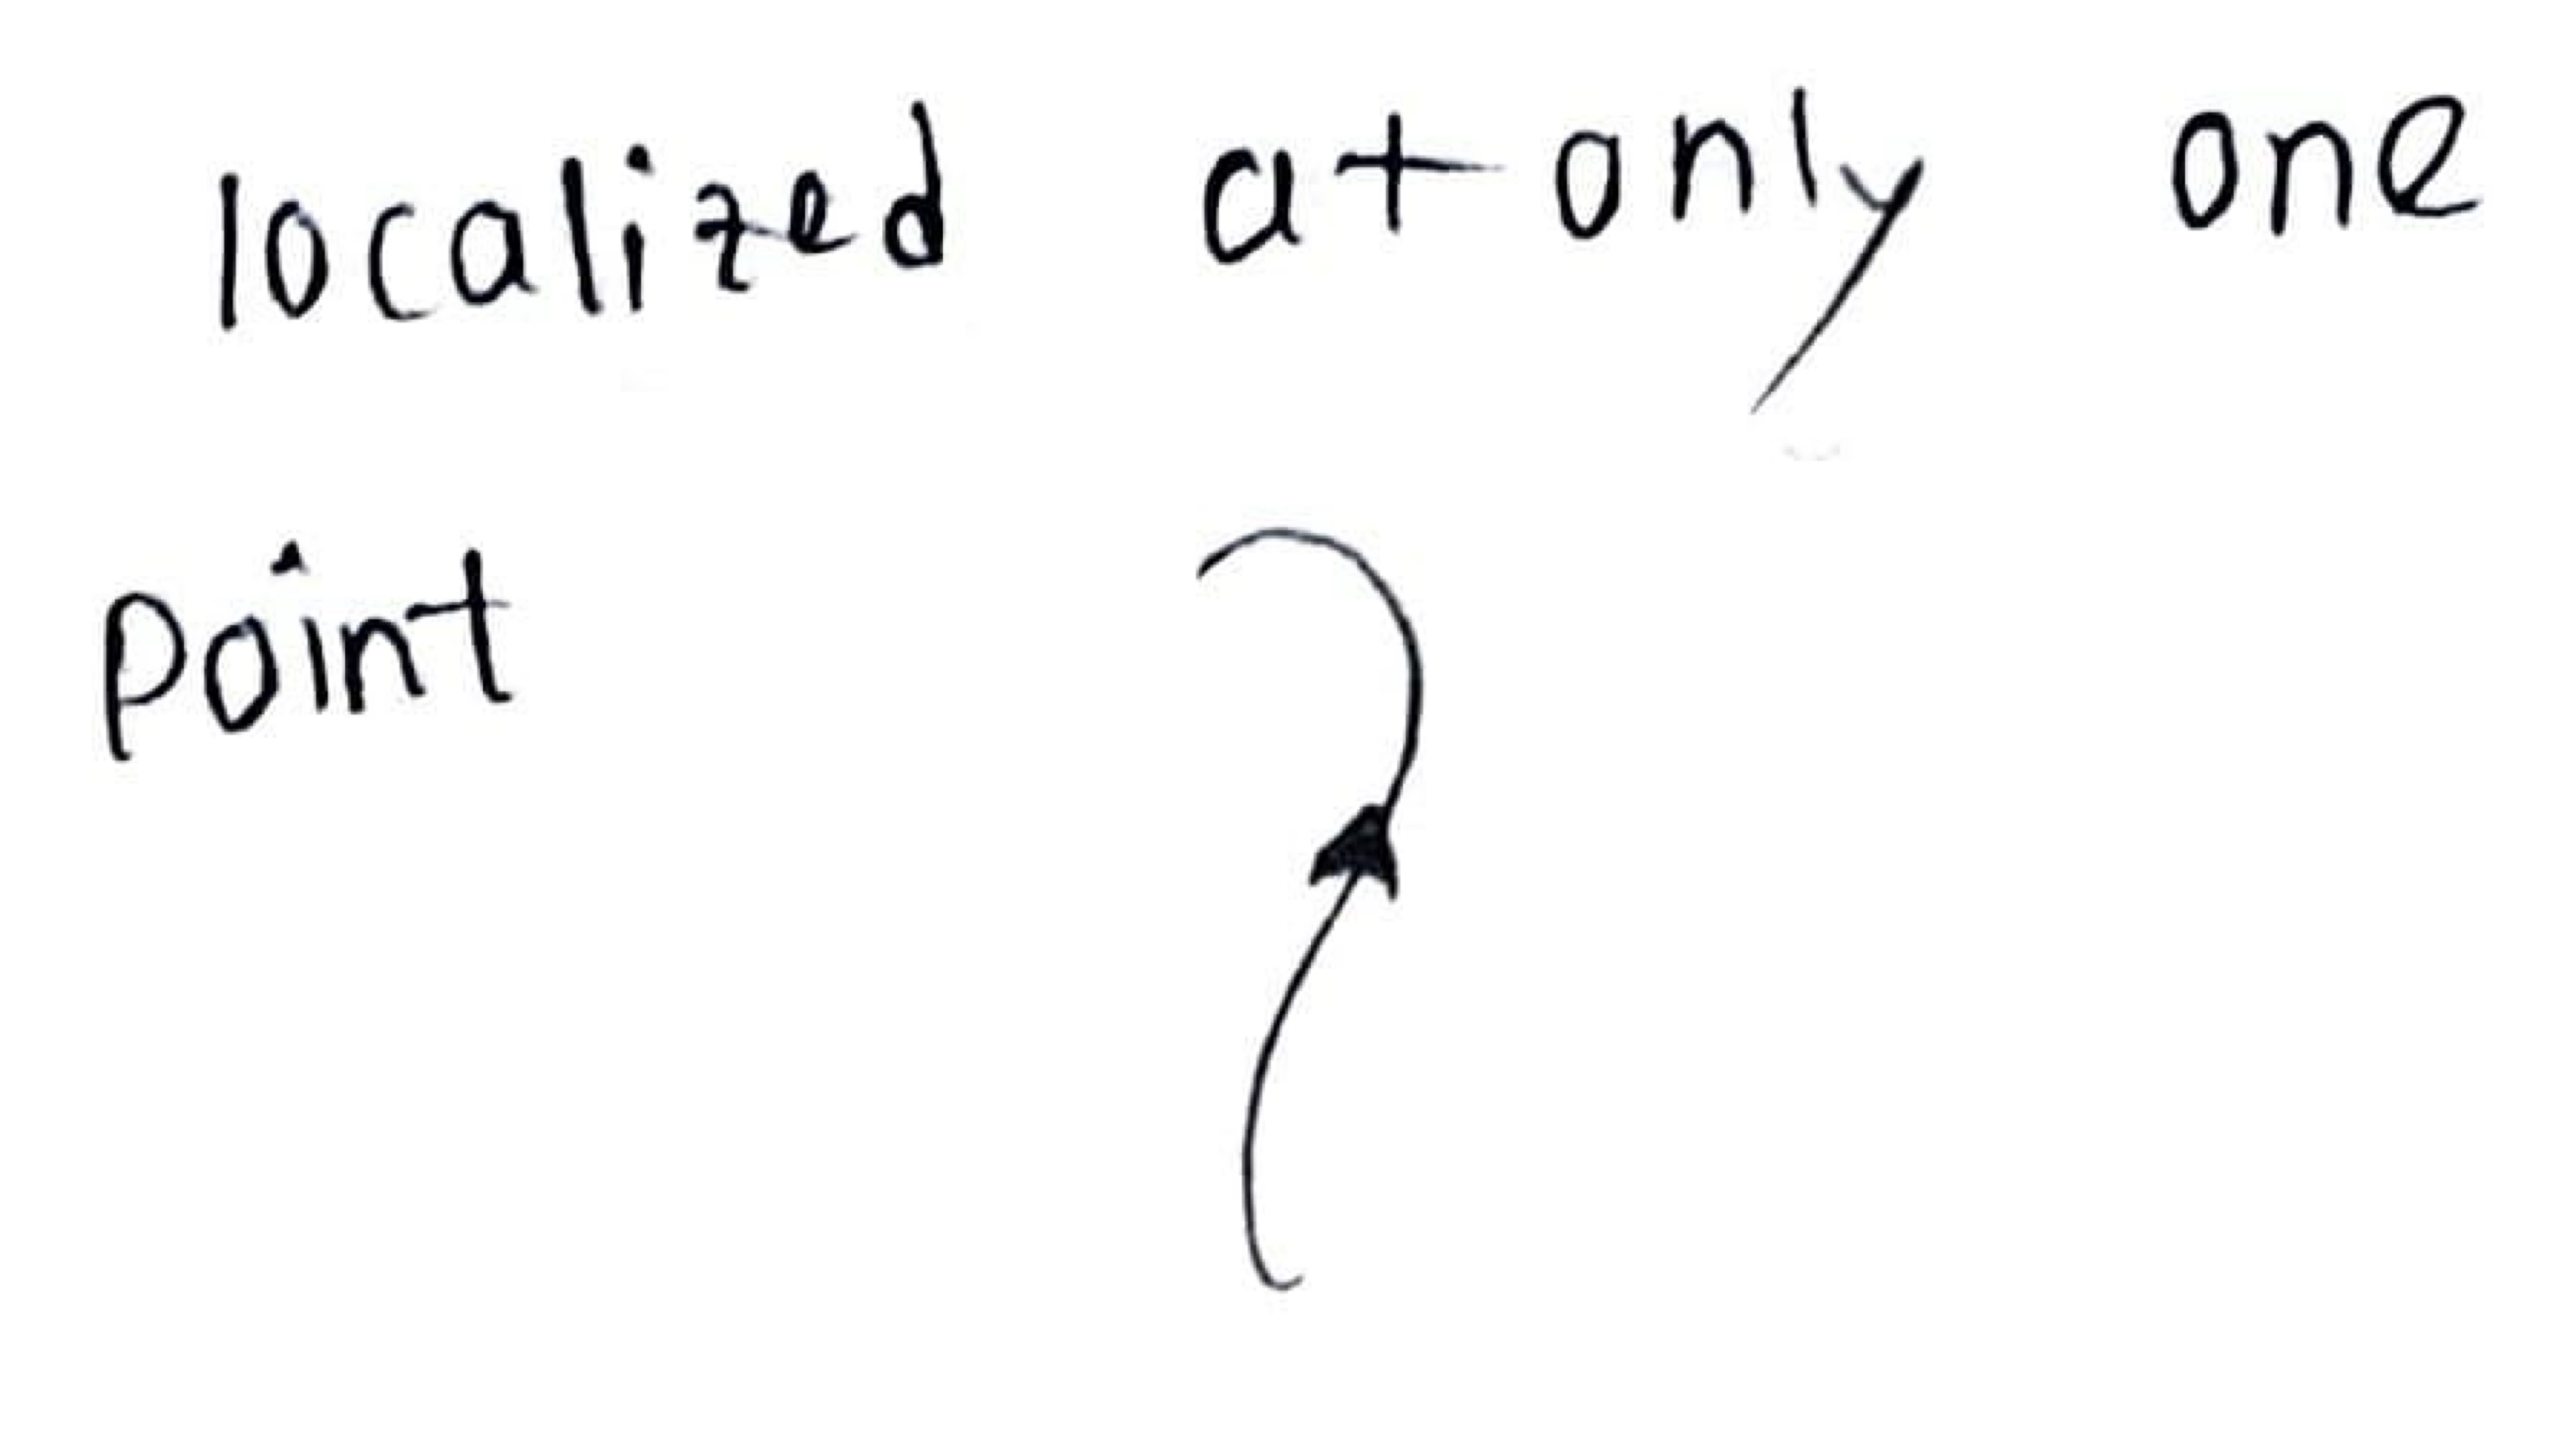
\includegraphics[width=\textwidth]{figures/L5_1.jpeg}
        \caption*{\underline{\textbf{Point}}\\[1ex]}
    \end{subfigure}
    \hfill
    % Subfigure 2: Field
    \begin{subfigure}[t]{0.4\textwidth}
        \centering
        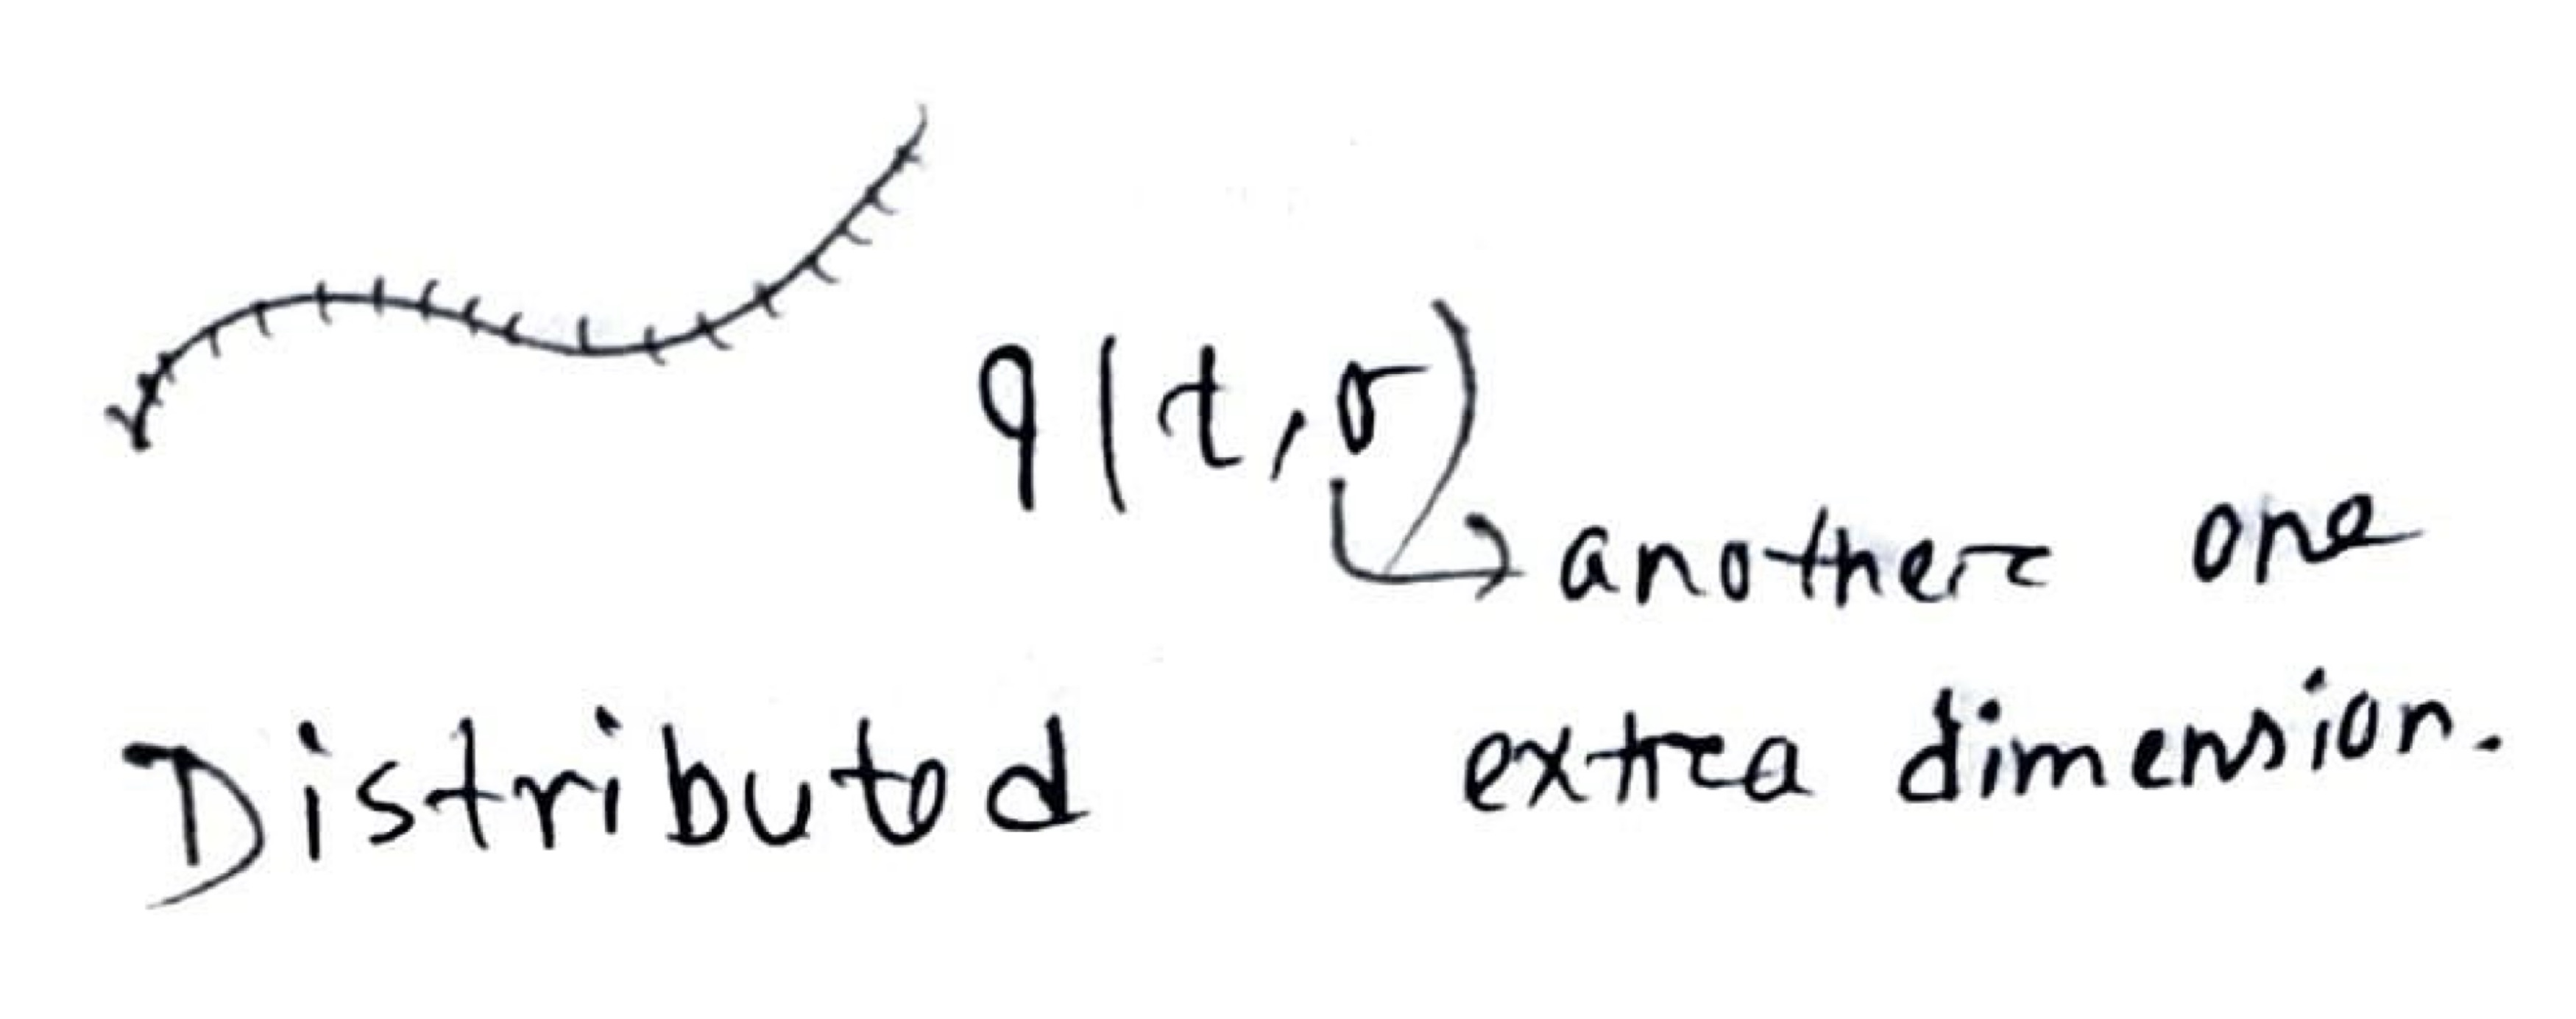
\includegraphics[width=\textwidth]{figures/L5_2.jpeg}
        \caption*{\underline{\textbf{Field}}\\[1ex]}
    \end{subfigure}    
    \caption*{}
\end{figure}
\vspace{-1cm}
\begin{itemize}
    \item \textbf{Point:} $q(t)$, in only one point.
    \item \textbf{Field:} $\phi(x) = \phi(t, x^i)$
\end{itemize}
% -----
Now action,
\[
S = \int \mathcal{L} \, dt = \int \left[ \int d^3x \, \mathcal{L}[\phi] \right] dt
\]
\subsection*{Tenet:}
\begin{enumerate}
    \item[(a)] Action is invariant under a set of transformations.
    \begin{itemize}
        \item Space-time symmetries (Poincaré and diffeomorphism)
        \item Internal symmetries
    \end{itemize}
    \[
    ds^2 = (dt)^2 - dx \cdot dx \quad \to \quad \text{Automorphism}
    \]
Now,
\vspace{-0.5cm}
\begin{center}
    $t \rightarrow -t$ \quad (time reversal) \\
    $~x \rightarrow -x$ \quad (space inversion)
\end{center}
These are discrete symmetries — \textbf{\textit{no conserved quantity}}. However if,
\[
x'^\mu = (\Lambda wx)^p + aw^p \quad \to \quad \text{continuous symmetry}
\]
According to Noether’s theorem, there's a conserved quantity for \textbf{\textit{continuous symmetry}}.

\begin{tcolorbox}[ title=Notes]
\subsection*{Coleman–Mandula Theorem (No-go Theorem):}
A sarcastic way to put it is - Internal symmetry cannot be married off to space-time symmetry within the framework of Lie group theory. \textbf{Example:} Generators:
\[
M = (J + P) + T
\]
Can't write like this so that:
\[
[J, T] \ne 0
\]
and
\[
JT^+ |-\frac{1}{2} \rangle = J~ |\frac{1}{2} \rangle
\]
\end{tcolorbox}

    \item[(b)] $\delta S = 0$ \quad $\to$ equation of motion
    \item[(c)] $\mathcal{L}[\phi]$ will be a polynomial of $\phi$ and its first-order derivative
\end{enumerate}
Now the Potential,
\[
V[\phi] = \phi^r + a \phi^3 + a' \phi^4 + \dots
\]
not  $e^\phi$ or $\sin\, \phi, cos\,\phi$ since we can take it in 1+1 dimension (In case $\phi(t, \sigma)$ )
\subsubsection*{Example:}
\[
S[\phi] = \alpha\, \phi_i \phi_i + \beta\, \partial \phi_i \, \partial \phi_i + \gamma_i\, \phi_i
\]
\[
= \int d^4x \left[~ \alpha \, \phi(x)\phi(x) + \beta \, \partial_\mu \phi(x) \partial^\mu \phi(x) + \gamma_i(x) \phi_i(x) ~\right]
\]
\[
[ \text{looking at this, it is too cumbersome without the DeWitt notation} ]
\]
Now taking variation,
\[
\delta S = 2\alpha\, \phi_i\, \delta \phi_i + 2\beta \, \partial \phi_i \, \delta(\partial \phi_i) + \gamma_i \,\delta \phi_i
\]
The variation is assumed to be between two differentiable configurations.
\begin{figure}[H]
    \centering
    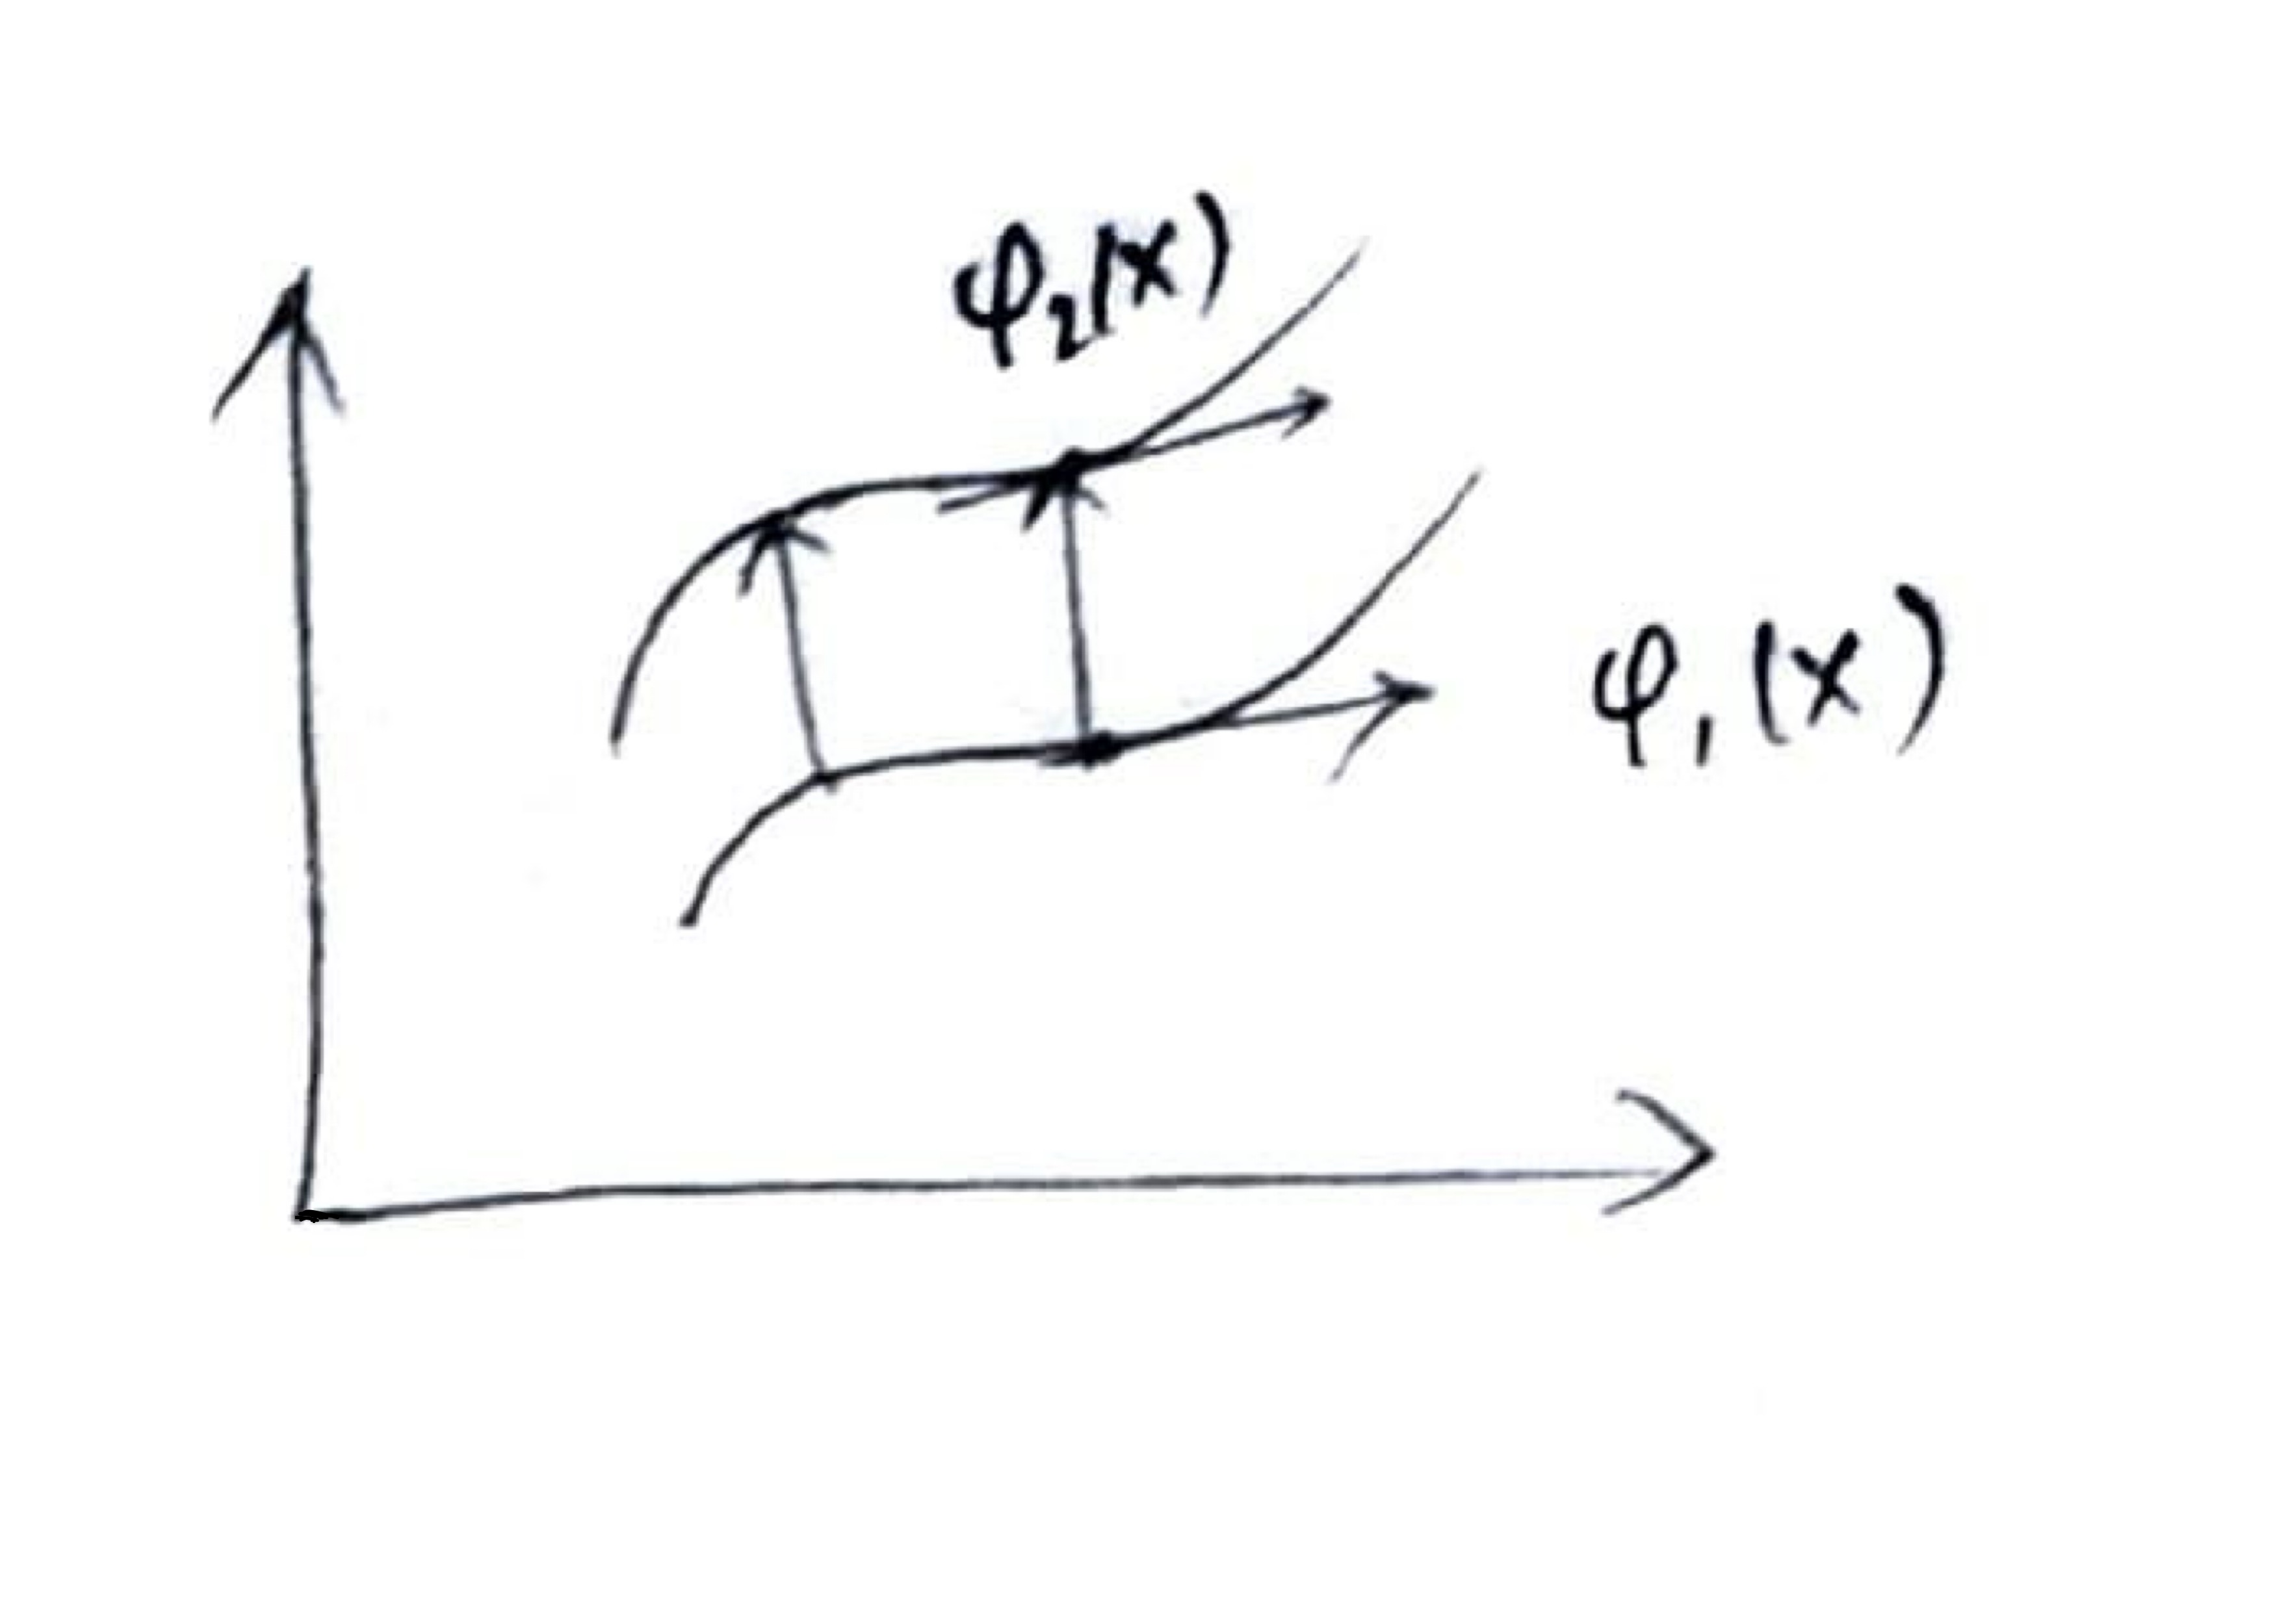
\includegraphics[width=0.4\linewidth]{L5_3.jpeg}
    \caption*{}
\end{figure}
\vspace{-1.5cm}
\begin{align*}
\delta \phi(x) &= \phi_2(x) - \phi_1(x) \\
\Rightarrow \partial \left[ \delta \phi(x) \right] &= \partial (\phi_2(x) - \phi_1(x)) \\
&= \partial \phi_2(x) - \partial \phi_1(x) \\ 
\therefore \partial(\delta \phi) &= \delta (\partial \phi)
\end{align*}
So, \textbf{\textit{variation and differentiation commute}}. Hence,
\begin{align*}
\delta S &= 2\alpha\, \phi_i\, \delta \phi_i + 2\beta \, \partial \phi_i \, \partial(\delta \phi_i) + \gamma_i \,\delta \phi_i \\
&= (2\alpha \,\phi_i + \gamma_i)\,\delta \phi_i - 2\beta \, \partial^2 \phi_i \, \delta \phi_i + \int (\partial \phi_i \, \partial \phi_i) \, d^4x \bigg|_{\text{boundary}} \\
&= \delta \phi_i \left( 2\alpha \phi_i + \gamma_i - 2\beta \, \partial^2 \phi_i \right)
\end{align*}
Since $\delta \phi_i$ is arbitrary,
\begin{align*}
& 2\alpha \phi_i + \gamma_i - 2\beta \, \partial^2 \phi_i = 0 \\
\Rightarrow & (2\beta \, \partial^2 - 2\alpha) \phi_i = \gamma_i
\end{align*}
\begin{itemize}
\item If $\alpha = \alpha(x)$:
\[
(2\beta \, \partial^2 - 2\alpha) \phi_i = \gamma_i
\quad \quad \text{(No problem)}\]
\item If $\beta = \beta(x)$:
\[
2 \partial\,(\beta \, \partial \phi_i) - 2\alpha_i \phi_i = \gamma_i
\]
\end{itemize} 
To match with the Klein-Gordon equation:,
\[
(\partial^2 + m^2)\phi = 0
\]
We need

\begin{align*}
    & 2\beta = +1 \\
    & 2\alpha = -1 \\
    & ~~\gamma = 0
\end{align*}
% \[
% 2\beta = 1 \quad , \quad 2\alpha = -1 \quad, \quad \gamma = 0
% \]
\begin{framed}
\textbf{Exercise:} Do the similar procedure for this action -
\[
S[\phi] = \alpha\, \phi_i \phi_i + \beta\, \partial \phi_i \, \partial \phi_i + \gamma_i\, \phi_i + K_i \partial \phi_i
\]
\textbf{Note:} The last term is important for $\pi$-meson.
\end{framed}
\begin{tcolorbox}[ title=Note]
A huge problem in Quantum Mechanics is linear independence which results in the potential \( V(x)\). $V(x)$ is not being spacetime invariant. A fundamental theory should not have the potential \( V(x) \).
\end{tcolorbox}

\textbf{Klein-Gordon Action:}

\begin{align*}
S &= \frac{1}{2} (\partial \phi)^2 - \frac{1}{2} m^2 \phi^2 + J\phi \\
  &= \int d^4x \left[ \frac{1}{2} \partial_\mu \phi \,\partial^\mu \phi - \frac{1}{2} m^2 \phi^2 + J(x)\, \phi(x) \right]
\end{align*}

\subsection{Electromagnetism}
Equation of Motion (EOM):
\[
\partial_\mu F^{\mu \nu} = j^\nu \quad \to \quad 4\text{ equations}
\]
Where,
\begin{align*}
F^{\mu \nu} &= \partial^\mu A^\nu - \partial^\nu A^\mu \\
\vec{B} &= \vec{\nabla} \times \vec{A} \\
\vec{E} &= -\vec{\nabla} A_0 - \frac{\partial \vec{A}}{\partial t}
\end{align*}
Thus we get two sets of equations from the equation of motion:
\begin{align*}
\vec{\nabla} \cdot \vec{E} &= \frac{\rho}{\varepsilon_0} \tag{M1} \\
\vec{\nabla} \times \vec{B} &= \mu_0 \vec{j} + \frac{\partial \vec{E}}{\partial t} \tag{M3}
\end{align*}
\newpage
The remaining two are found from:
\[
\partial_{[\mu}F_{\nu \lambda ]} = \partial_\mu F_{\nu \lambda} + \partial_\nu F_{\lambda \mu} + \partial_\lambda F_{\mu \nu} = 0 \tag*{[Bianchi identity]}
\]
\begin{align*}
\vec{\nabla} \cdot \vec{B} &= 0 \tag{M2} \\
\vec{\nabla} \times \vec{E} &= -\frac{\partial \vec{B}}{\partial t} \tag{M4}
\end{align*}
\begin{tcolorbox}[ title=Notes]
\begin{itemize}
    \item There are total 8 Maxwell’s (scaler) equations — 2 scalar divergence equations, 6 scalar components from the 2 vector curl equations.
    \item The vector equations evolve with time; their validity is confirmed from the previous two equations.
    \item Maxwell's EOM are equivalent to Hamilton's EOM, not the Lagrange's.
\end{itemize}
\end{tcolorbox}
Now for the action,
\[
S = \int \mathcal{L}(\phi, \partial \phi) \sqrt{-g}~ d^4x
\]
The determinant of $g$ is negative so we put a minus sign inside to make the $(-g)$ positive. However we omit it in flat space:
\begin{align*}
\delta S &= \int \left[ \frac{\partial \mathcal{L}}{\partial \phi} \delta \phi + \frac{\partial \mathcal{L}}{\partial(\partial_\mu \phi)} \delta(\partial_\mu \phi) \right] d^4x \\
&= \int \left[ \frac{\partial \mathcal{L}}{\partial \phi} \delta \phi + \frac{\partial \mathcal{L}}{\partial(\partial_\mu \phi)} \partial_\mu(\delta \phi) \right] d^4x \\
&= \int \left[ \frac{\partial \mathcal{L}}{\partial \phi} - \partial_\mu \left( \frac{\partial \mathcal{L}}{\partial(\partial_\mu \phi)} \right) \right] \delta \phi \, d^4x 
+ \int d^3x~\eta^\mu \frac{\partial \mathcal{L}}{\partial(\partial_\mu \phi)} \delta \phi \\
&= \quad0 \quad\left( \int d^3x~\eta^\mu \frac{\partial \mathcal{L}}{\partial(\partial_\mu \phi)} \delta \phi = 0 \to \text{ Dirichlet condition} \right)
\end{align*}
\begin{tcolorbox}[ title=Verifying Dirichlet condition]
Let's verify this,
\begin{align*}
\nabla \cdot (\psi \nabla \phi) &= \nabla \psi \cdot \nabla \phi + \psi \nabla^2 \phi \\
\Rightarrow \int \nabla \phi \cdot \nabla \psi~d^3x &= -\int \psi \, \nabla^2 \phi~d^3 x +\int\nabla \cdot(\psi \nabla \phi)~ d^3 x \\
&=  -\int \psi \, \nabla^2 \phi~d^3 x +\int \psi (n\cdot\nabla) \phi~ d \mathcal{S}
\end{align*}
\end{tcolorbox}
% ---
\begin{tcolorbox}[ title=Post-class discussions]
\begin{figure}[H]
    \centering
    \vspace{-0.7cm}
    % Time-like Space
    \begin{minipage}[t]{0.6\textwidth}
    \vspace{-2.5cm}
        \textbf{Time-like Space:}
        \begin{itemize}
            \item Perpendicular is in time-like direction.
        \end{itemize}
    \end{minipage}%
    \hfill
    % \vspace{-1cm}
    \begin{minipage}[t]{0.35\textwidth}
        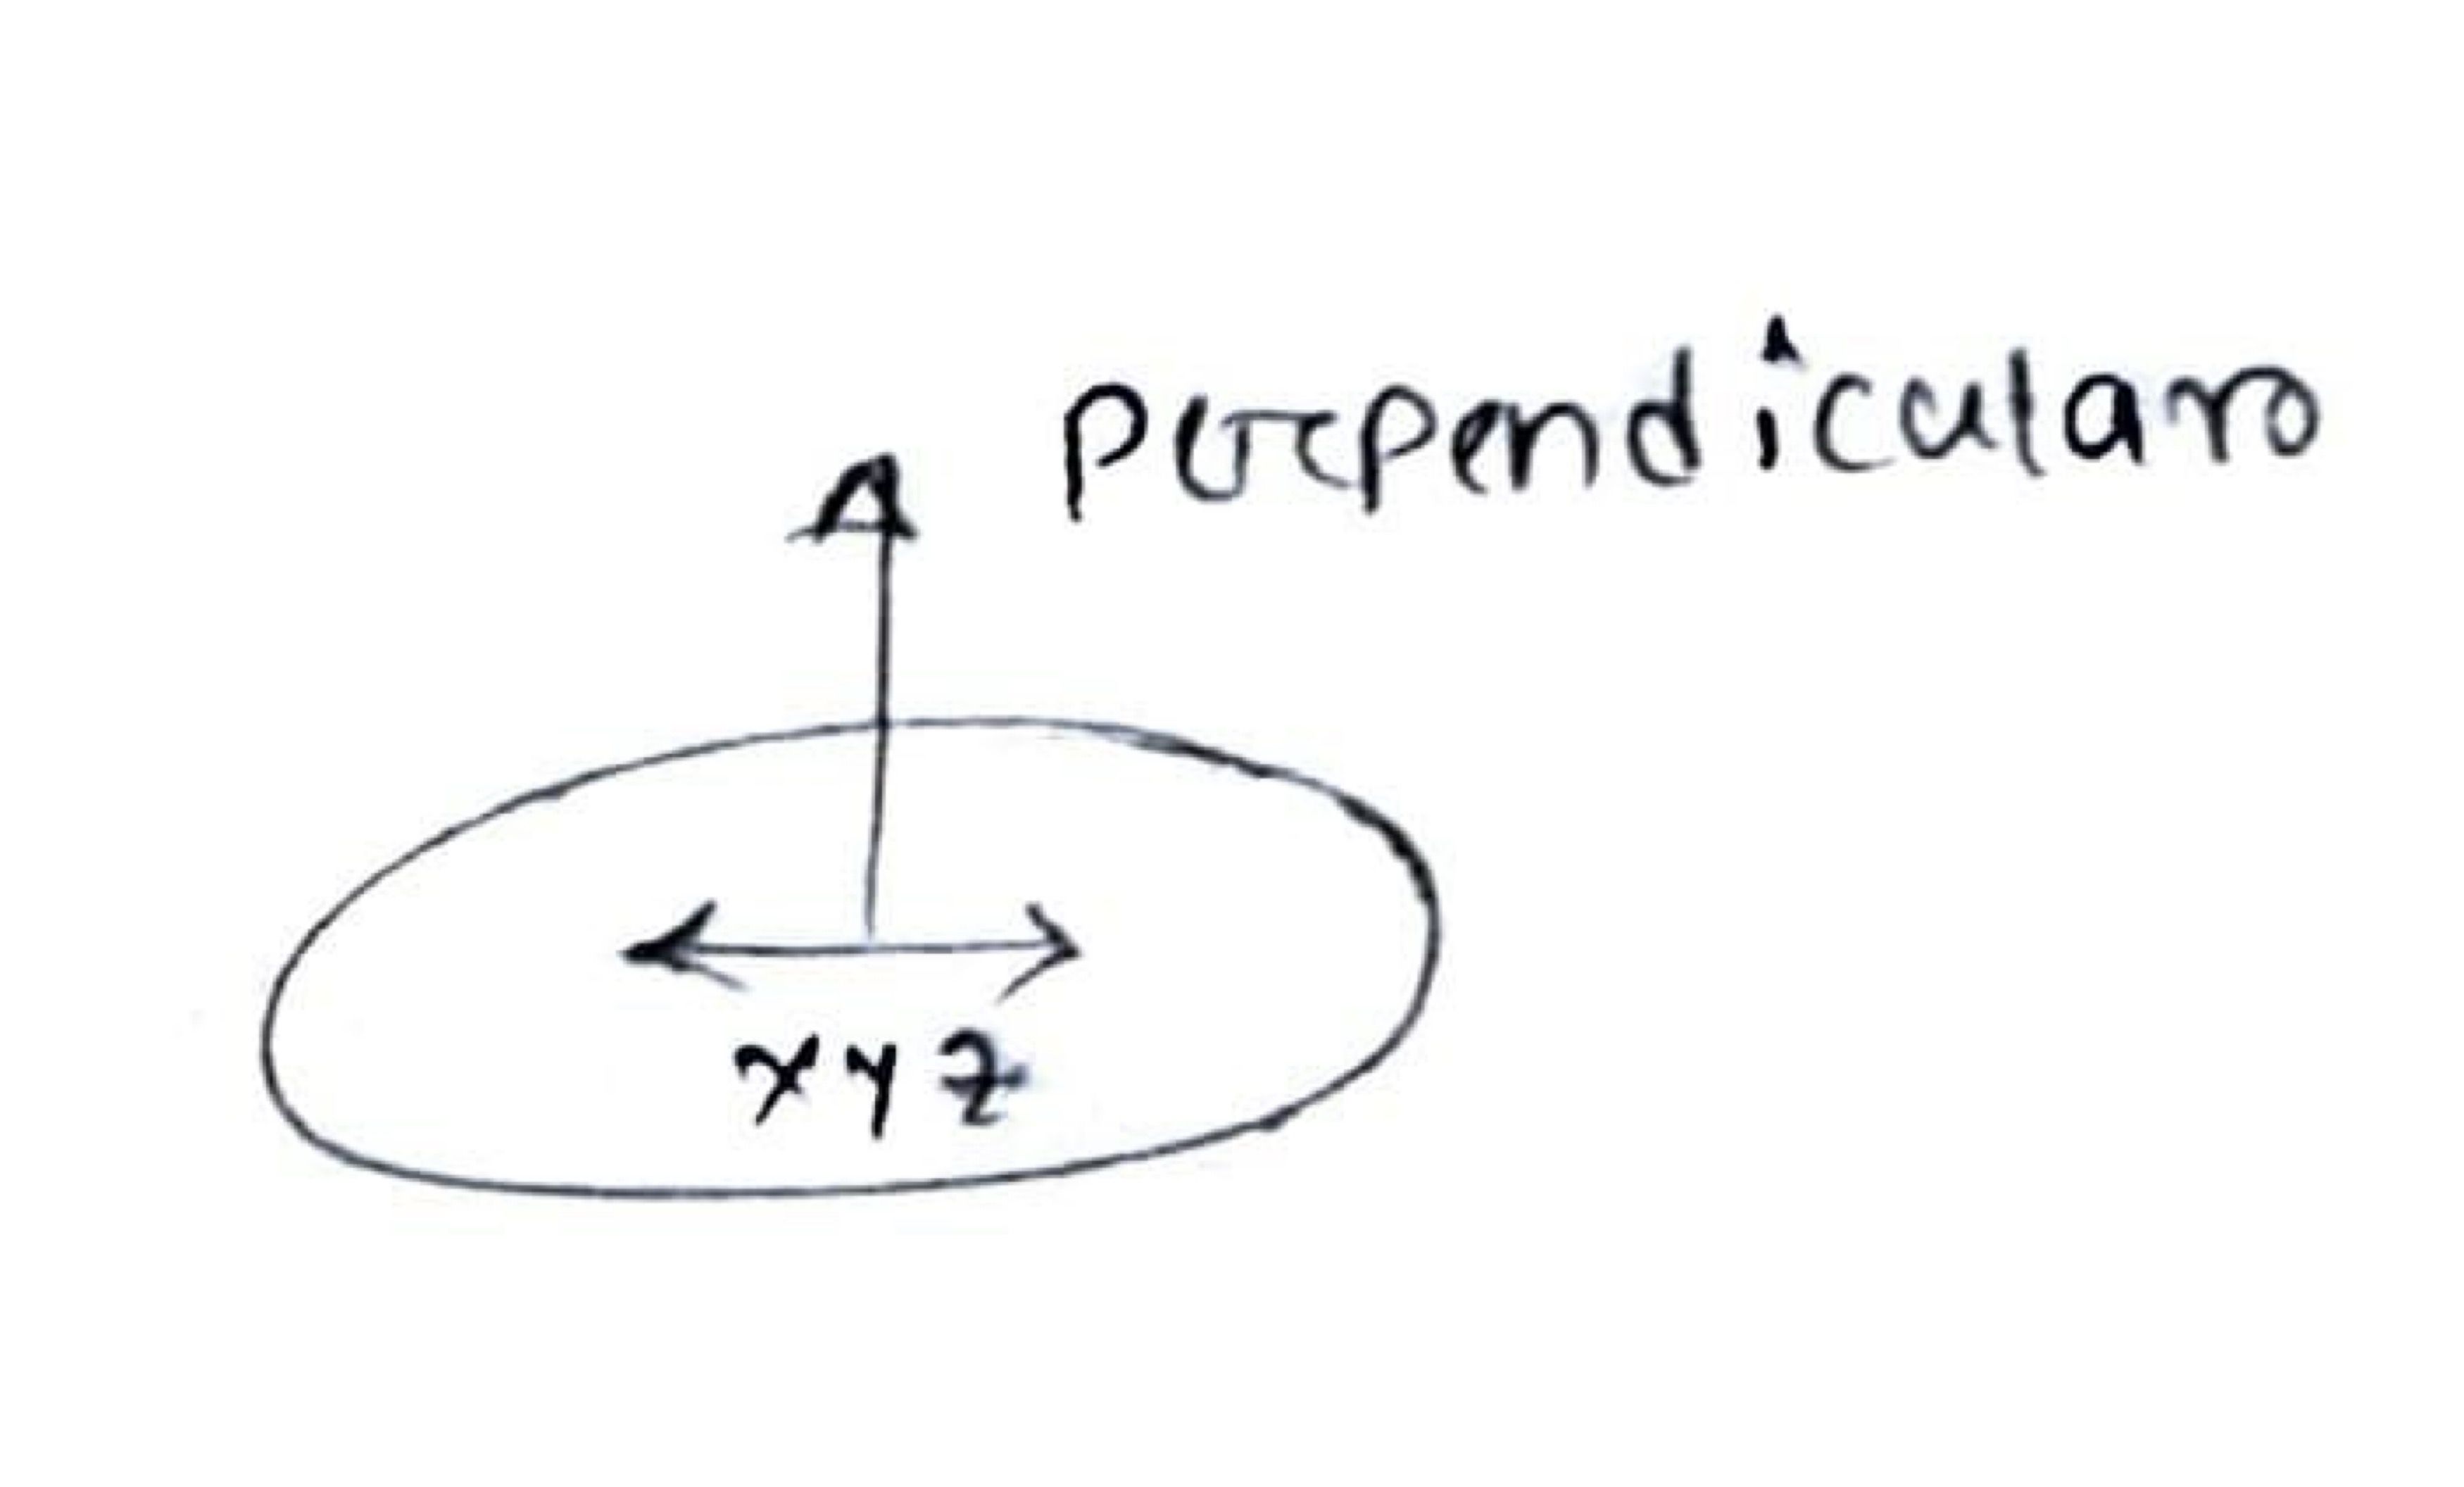
\includegraphics[width=\linewidth]{figures/L5_5.jpeg}
    \end{minipage}
    % Space-like Space
    \begin{minipage}[t]{0.6\textwidth}
    \vspace{-3.5cm}
        \textbf{Space-like Space:}
        \begin{itemize}
            \item Perpendicular is in z-direction.
        \end{itemize}
    \end{minipage}%
    \hfill
    \begin{minipage}[t]{0.35\textwidth}
        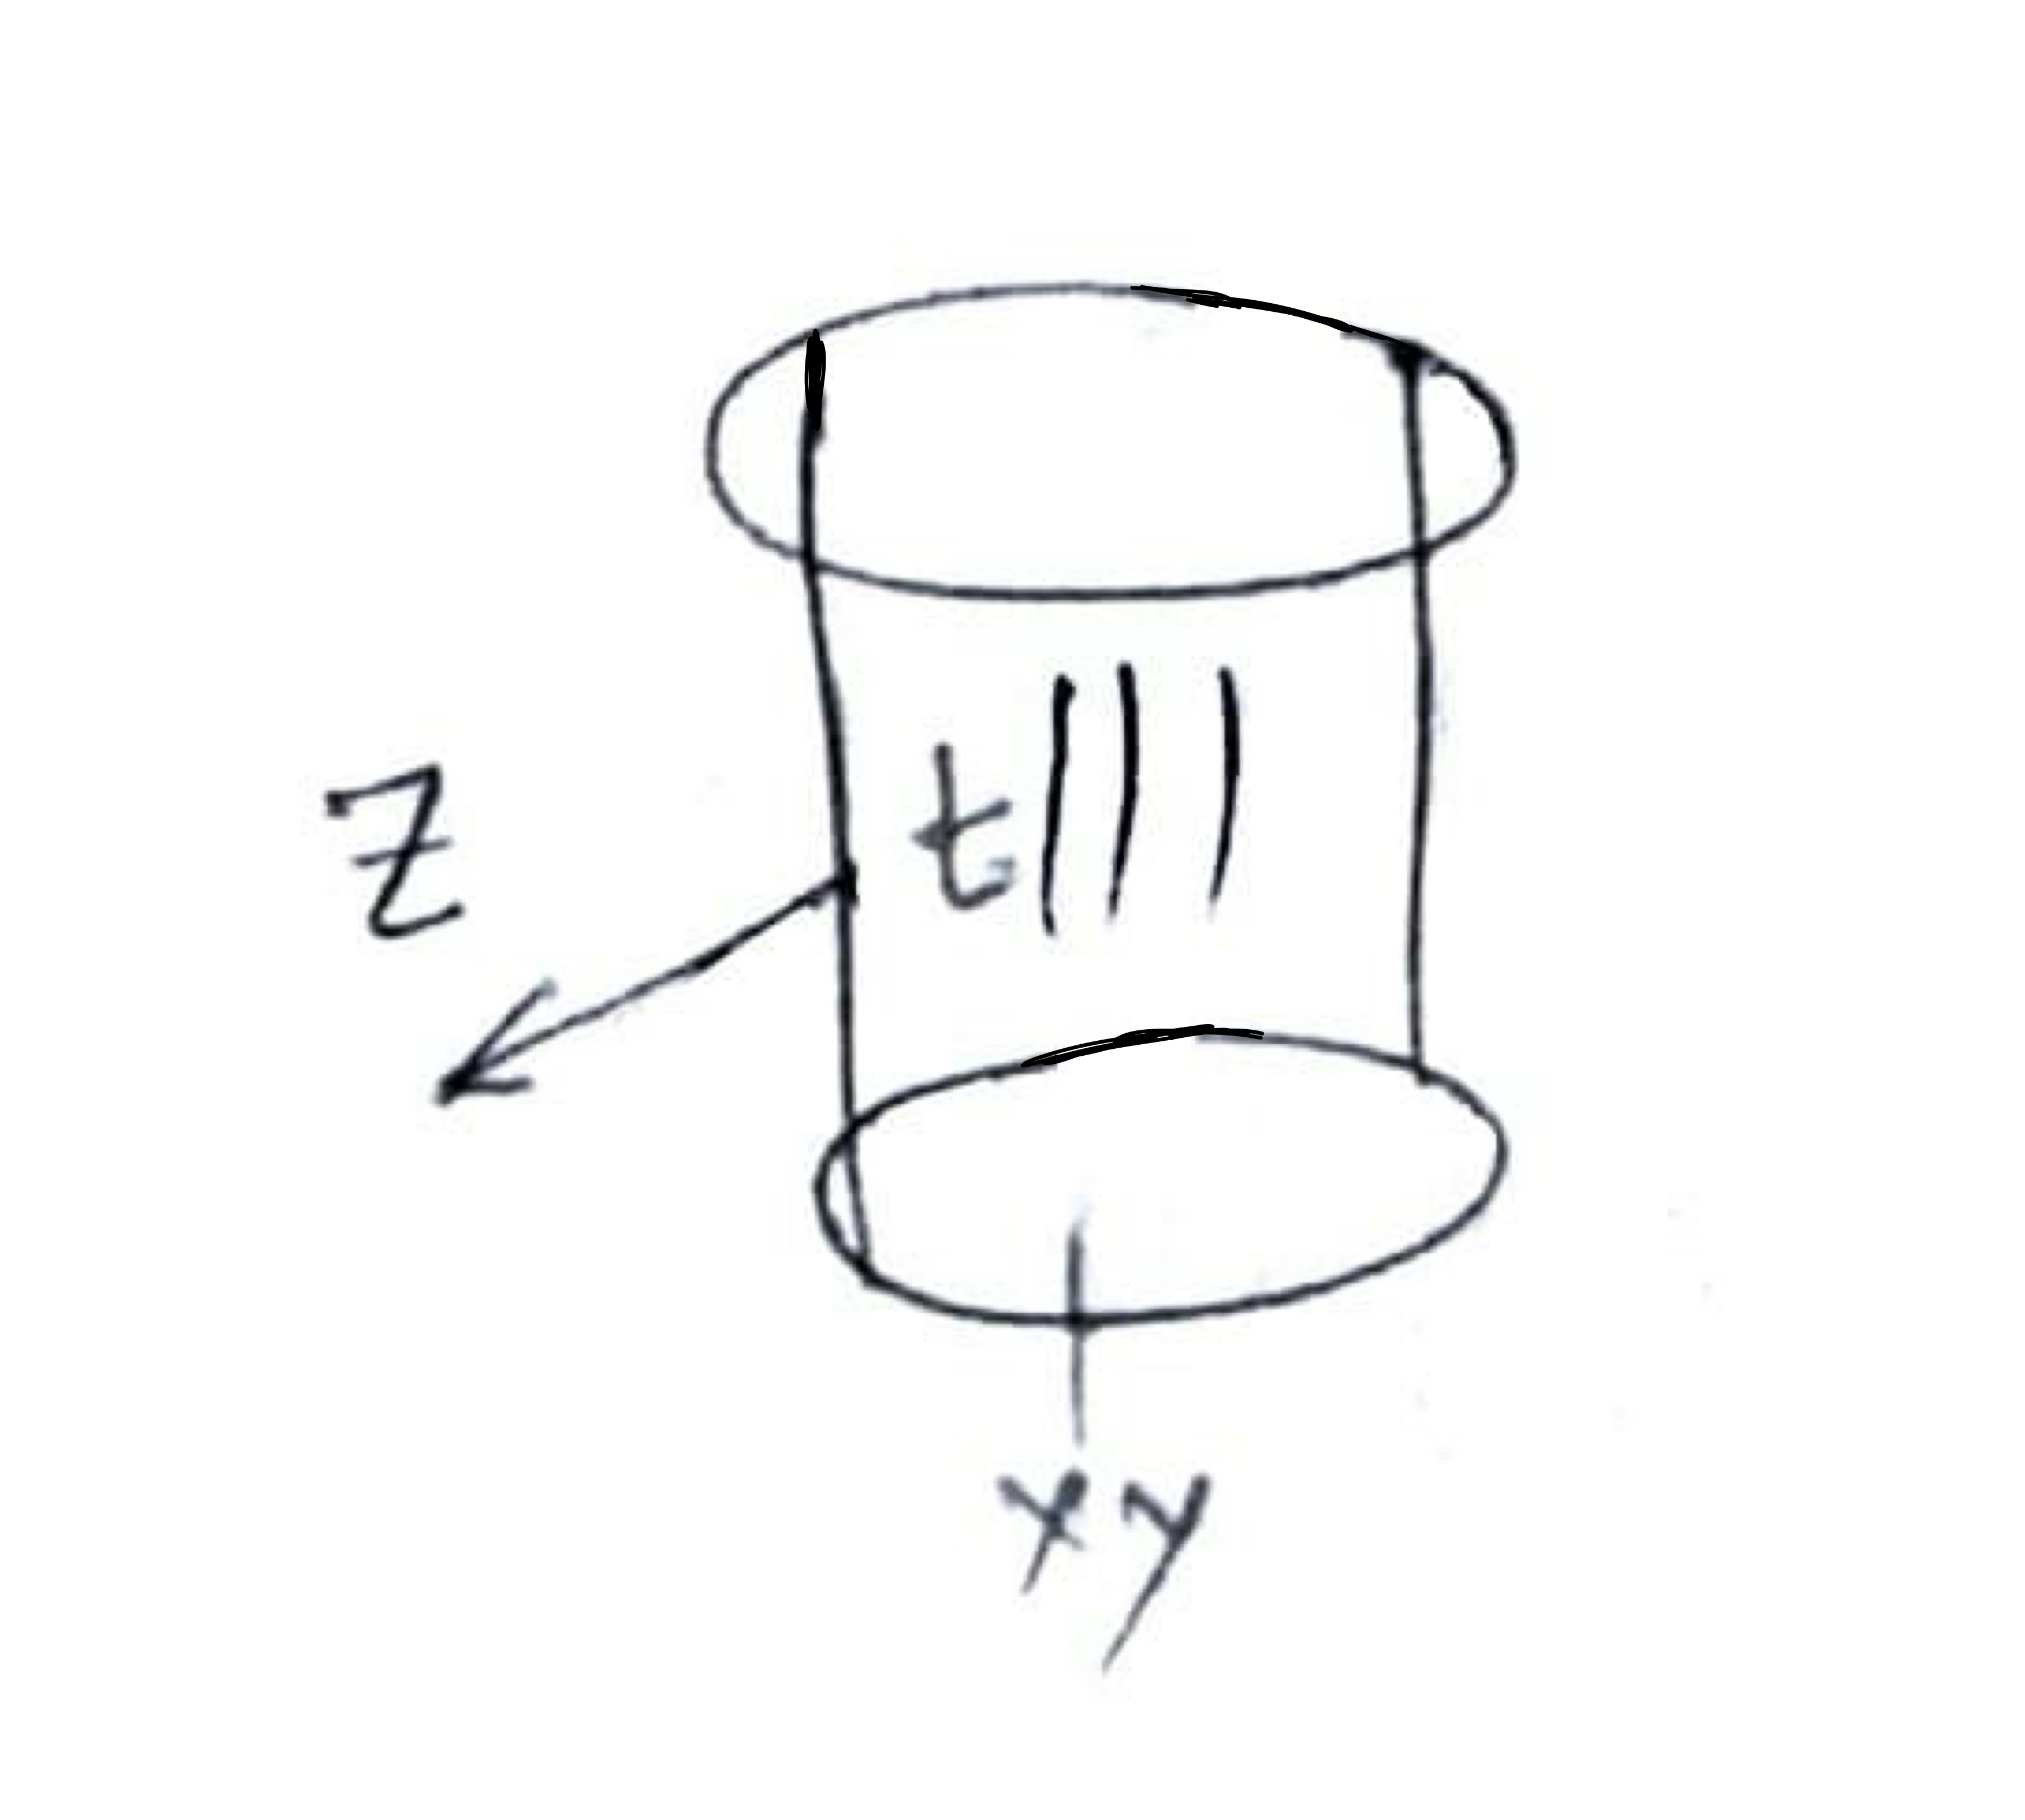
\includegraphics[width=\linewidth]{figures/L5_4.jpeg}
    \end{minipage}
    % Null-like Space
    \begin{minipage}[t]{0.6\textwidth}
    \vspace{-3cm}
        \textbf{Null-like Space:}
        \begin{itemize}
            \item Null object's perpendicular is also null.
            \item E.g., light ray.
        \end{itemize}
    \end{minipage}%
    \hfill
    \begin{minipage}[t]{0.35\textwidth}
        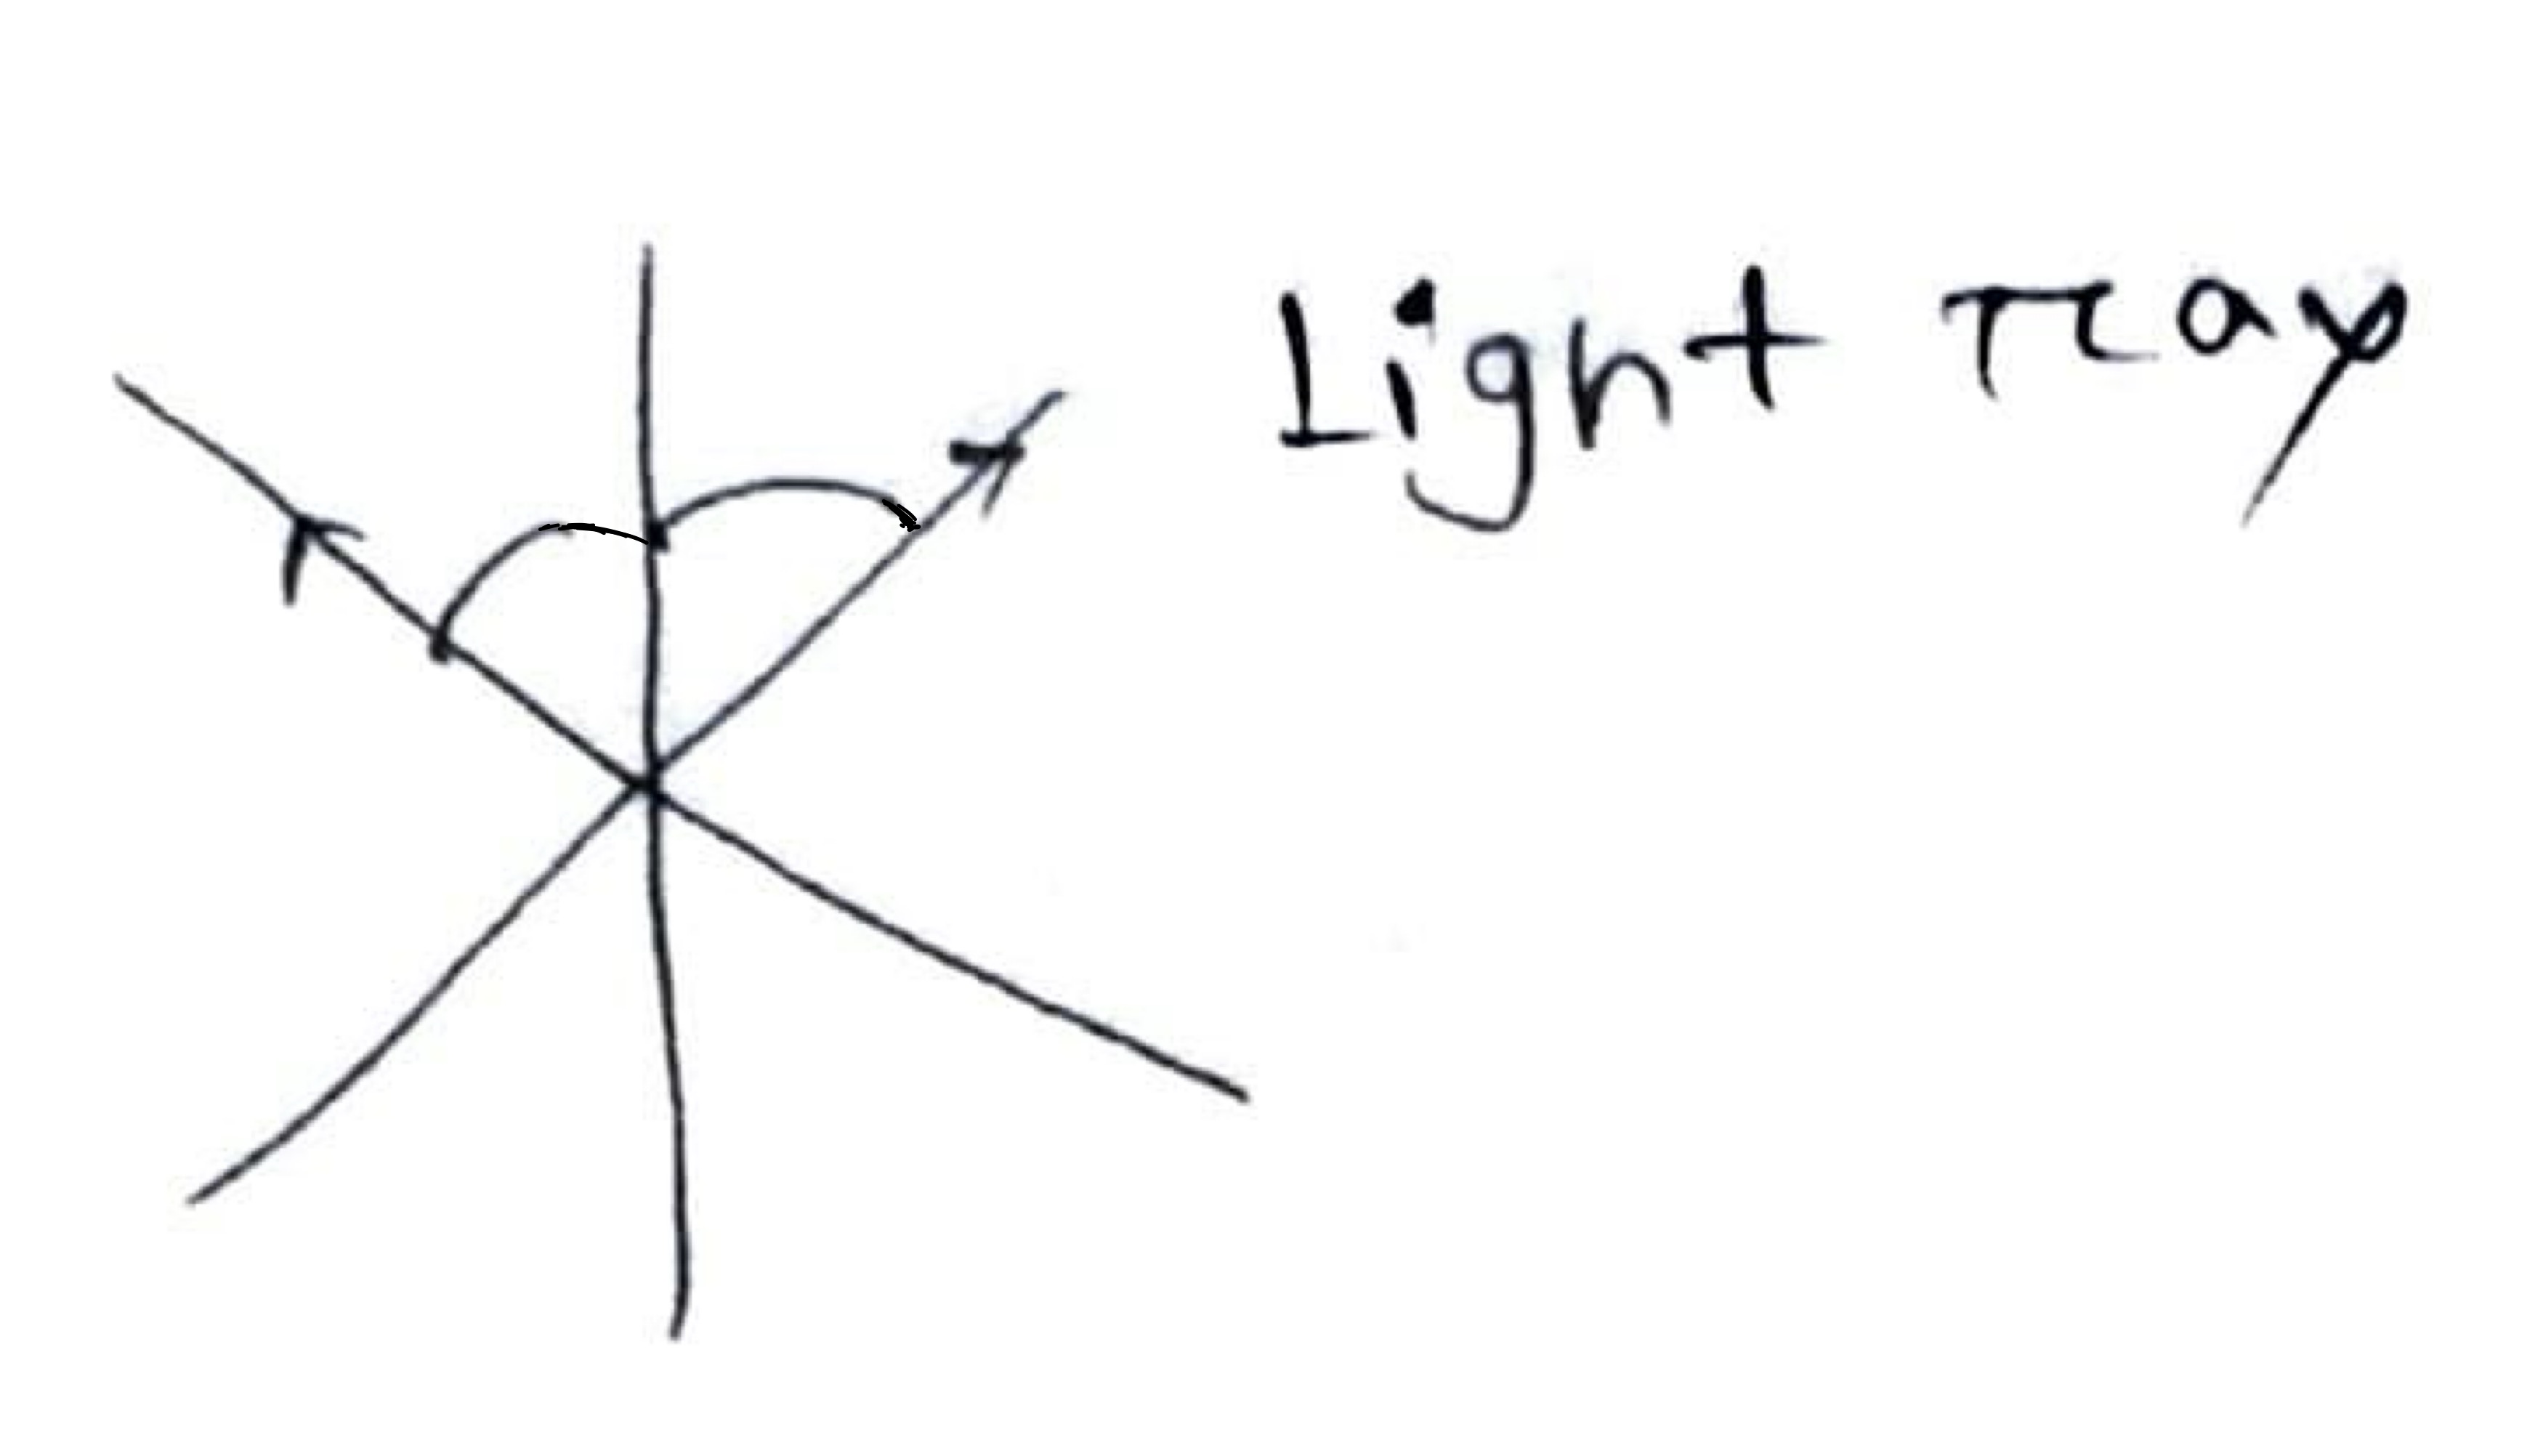
\includegraphics[width=\linewidth]{figures/L5_6.jpeg}
    \end{minipage}

\end{figure}
\end{tcolorbox}
\newpage

\stepcounter{section}
\renewcommand{\thesection}{\arabic{section}}
\fancysection{(\textit{\textbf{Class-9})} Lecture \textbf{6}: Sat, June 28, 2025}{\textbf{\textit{Gauge Theory}}}
%---
% For a free particle, $m = 1$. The Lagrangian, 
% \[
% \mathcal{L} = \frac{1}{2} m \dot{q}^2 \rightarrow q, \dot{q}~\text{as independent}
% \]
% Also, if 
% \[
% \mathcal{L} = -\frac{1}{2}q\,\ddot{q} \to q, \dot{q}~\text{as independent}
% \]

% Therefore, $\delta \mathcal{L} = 0$ implies
% \begin{align*}
% &\quad \frac{\partial \mathcal{L}}{\partial q} - \frac{d}{dt} \left( \frac{\partial \mathcal{L}}{\partial \dot{q}} \right) + \frac{d^2}{dt^2} \left( \frac{\partial \mathcal{L}}{\partial \ddot{q}} \right) = 0 \\
% &\Rightarrow 0 - \frac{d}{dt} \left( \frac{1}{2} \times 2m \dot{q} \right) + \frac{d^2}{dt^2}(0) = 0  \quad [\,\because \ddot{q}=0~]\\
% & \Rightarrow \frac{d}{dt}(m \dot{q}) = 0
% \Rightarrow m \ddot{q} = 0
% \Rightarrow \ddot{q} = 0 
% \end{align*}
% Now, if 
% \[
% \mathcal{L} = \frac{1}{2} \ddot{q}^2 \Rightarrow \frac{d^2}{dt^2} \left( \frac{\partial \mathcal{L}}{\partial \ddot{q}} \right) = \frac{d^2}{dt^2} (\ddot{q}) = 0
% \]

% \[
% \Rightarrow \text{No Unique Lagrangian!}
% \]

\subsection{Gauge Field}
\subsubsection{Free Field}
Maxwell field $\equiv$ EM field \\
Electromagnetism is \textbf{not} a theory of \textbf{field strength tensor}, but a \textbf{theory of potential}.

Now, 
\[
\mathcal{L} = -\frac{1}{4} F^{ab} F_{ab} \quad;\quad F_{ab} = \partial_{[a}A_{b]} = \partial_a A_b - \partial_b A_a
\]
\begin{tcolorbox}[ proofbox, title=Note about the factor-$\frac{1}{2}$ ]
\begin{itemize}
    \item If we put $\frac{1}{4}$ in the Lagrangian, the $\frac{1}{2}$ is necessary in $F_{ab}$, otherwise we can omit it.
    \item `$\frac{1}{2}$' was also used in \textit{Penrose's} book
\end{itemize}
\end{tcolorbox}
To find the equation of motion from the Lagrangian, we vary $A$,
\begin{align*}
\delta \mathcal{L} &= -\frac{1}{4} F^{ab}~\delta F_{ab}  -\frac{1}{4} \delta F_{ab}~ F^{ab} \\
&= -\frac{1}{2} F_{ab}~ \delta F^{ab} \\
&= -\frac{1}{2} F_{ab}~\delta ( \partial^a A^b - \partial^b A^a ) \\
&= -F_{ab}~ \delta (\partial^a A^b) \tag{9.1} \label{9.1} \\
\therefore \delta \mathcal{L}&= -F_{ab}~ \partial^a (\delta A^b) =0 \quad [\text{however, } \delta A^b \ne 0] \\
\therefore \partial^a &F_{ab} = 0 \quad \text{(Free Maxwell Equation)}
\end{align*}
\begin{tcolorbox}
Derivation of \eqref{9.1}
\begin{align}
F_{ab}~(\partial^a C^b - \partial^b C^a ) &= F_{ab}~\partial^a C^b - F_{ab}~\partial^b C^a  \\
&= F_{ab}~\partial^a C^b - F_{ba}~\partial^a C^b \\
&= F_{ab}~\partial^a C^b + F_{ab}~\partial^a C^b \quad [\because F_{ab} = -F_{ba} ] \\
\therefore F_{ab}~(\partial^a C^b - \partial^b C^a ) &= 2F_{ab}~\partial^a C^b = 2F_{ab}~\partial^a A^b \quad[ C\to A ]
\end{align}
\end{tcolorbox}
\subsubsection{In Presence of a Source}
\begin{align*}
&\partial^a F_{ab} = J_b \\
\Rightarrow ~&\partial^a F_{ab} - J_b = 0
\end{align*}
and variation:
\[
F_{ab}~\partial^a (\delta A^b) - J_b \, \delta A^b = 0
\]
Thus in presence of a source the Lagrangian becomes,
\[
\mathcal{L} = -\frac{1}{4} F_{ab} F^{ab} - J_b \,A^b
\]
\[
J_b \, A^b \to \text{Interaction term}
\]
\begin{tcolorbox}[ proofbox, title=Notes ]
\begin{itemize}
    \item Everything else other than the gauge field is matter.
    \item In the theory of gravitation, electromagnetism will act as a matter.
\end{itemize}
\end{tcolorbox}

\begin{figure}[H]
    \centering
    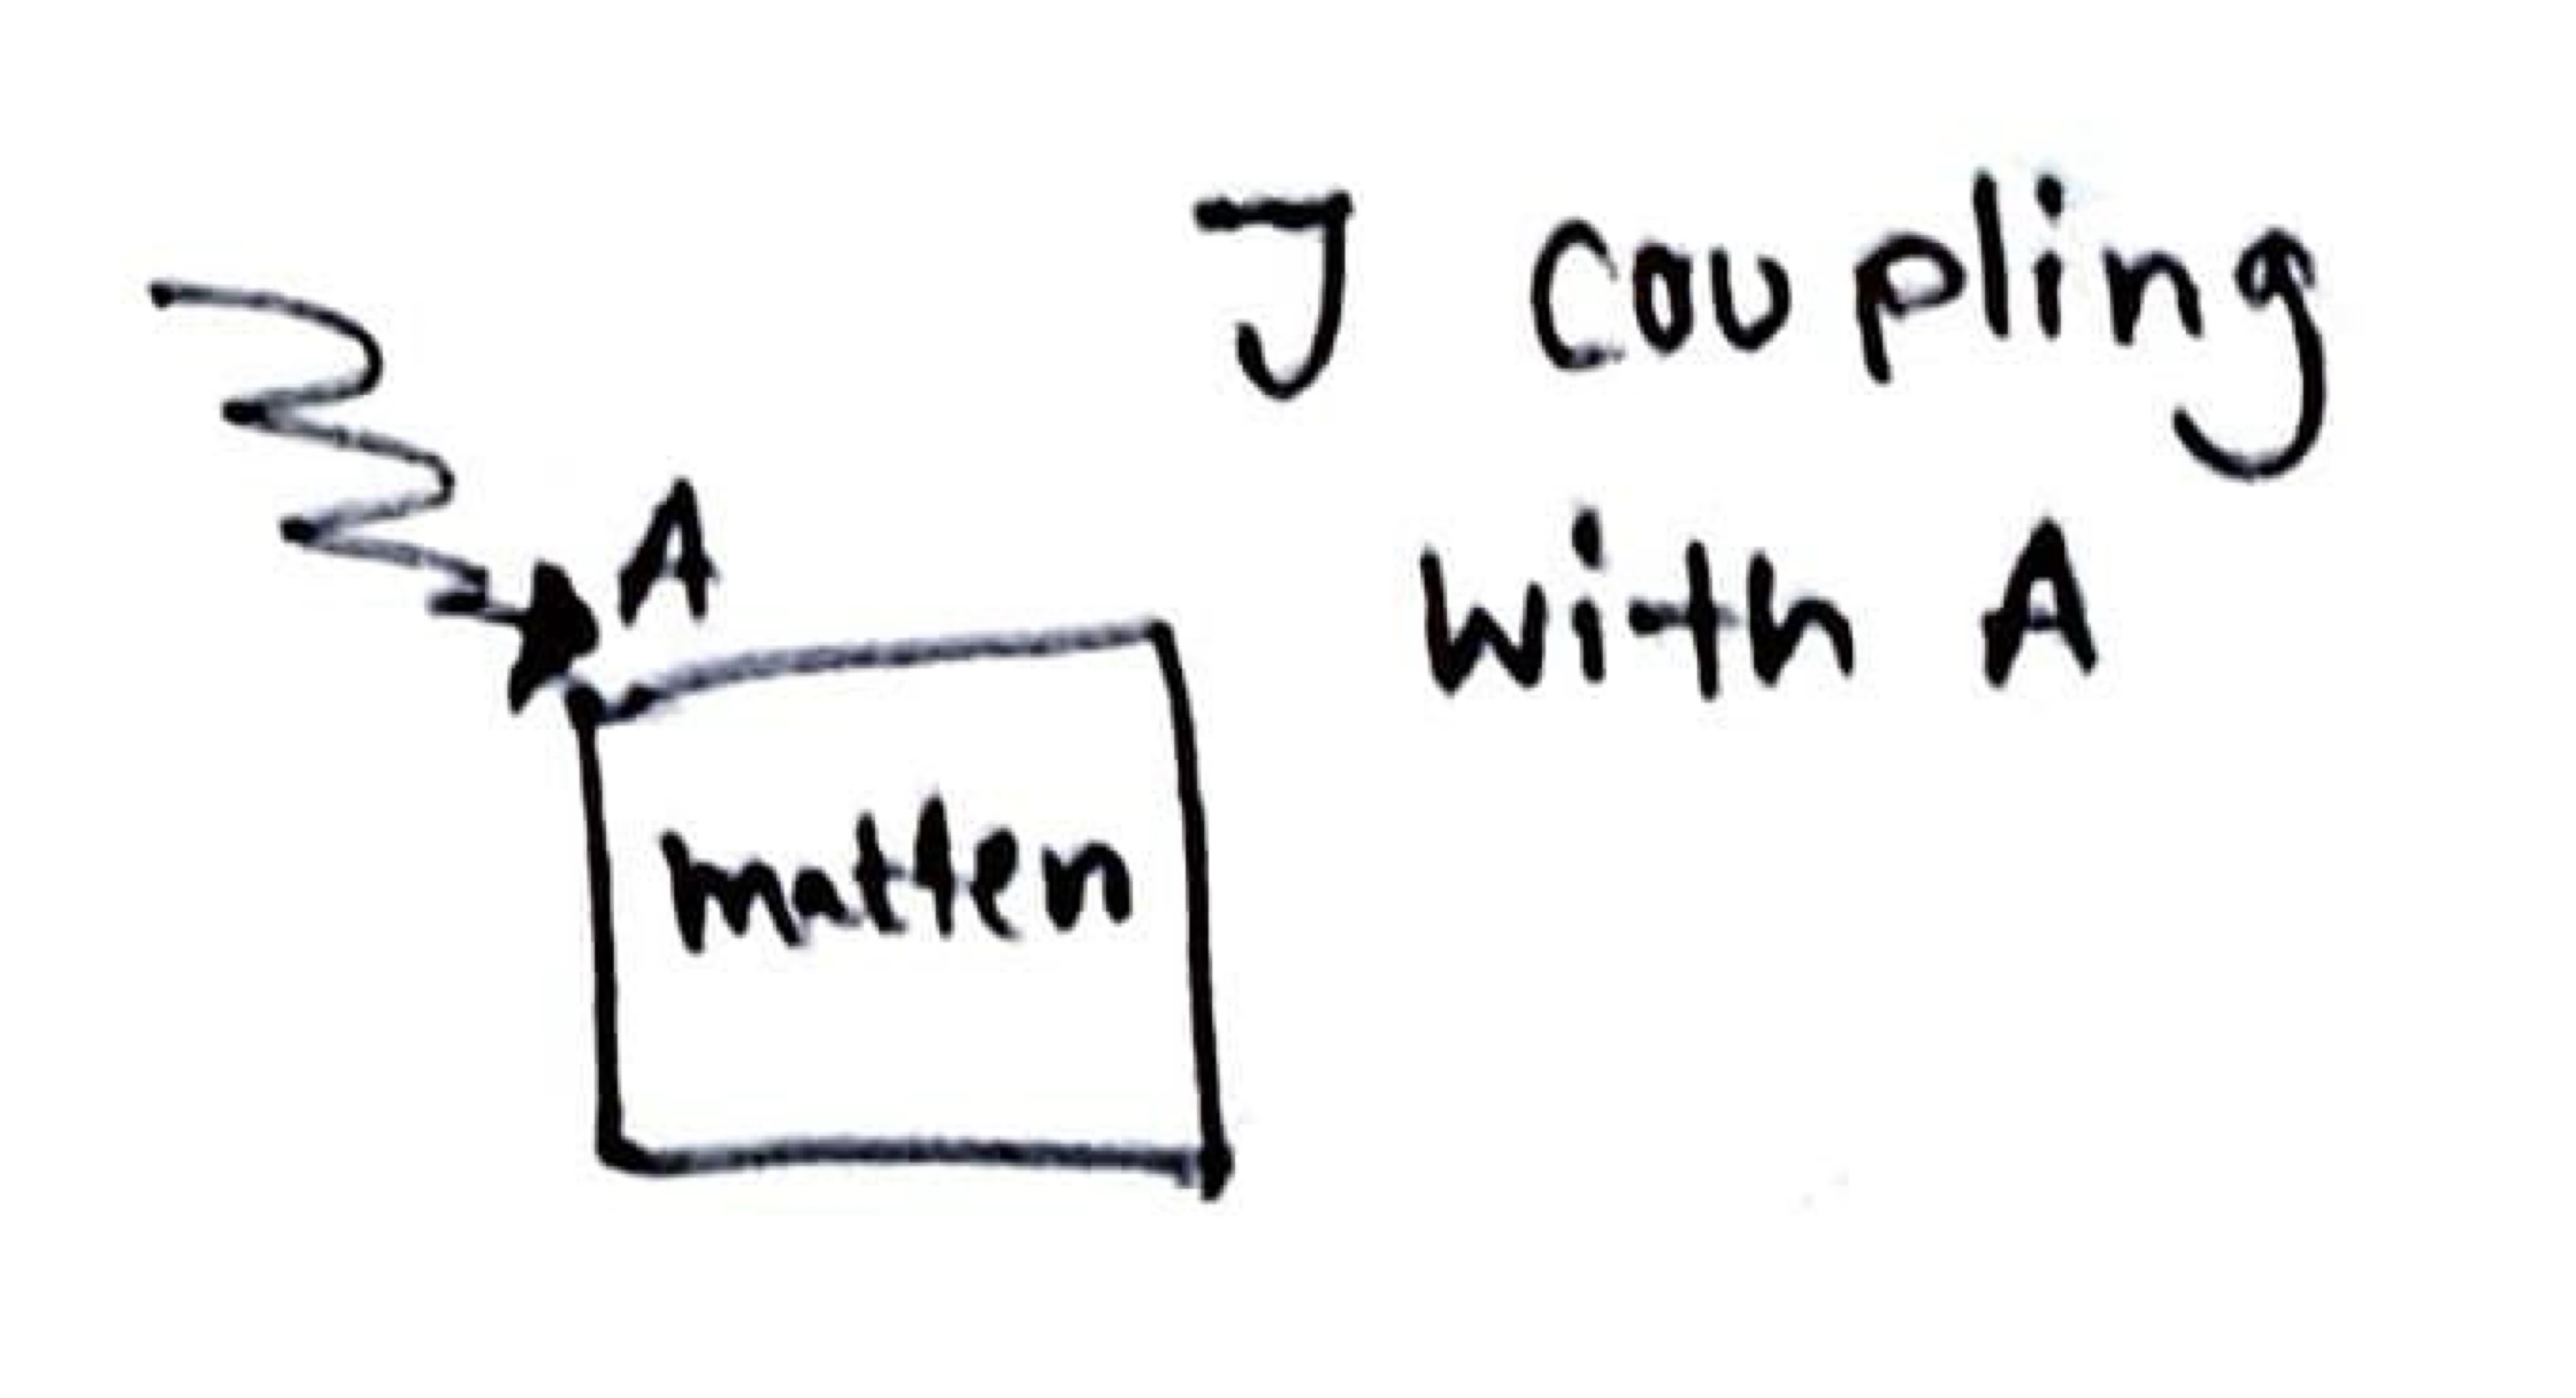
\includegraphics[width=0.3\linewidth]{figures/C09_1.jpeg}
    \caption*{}
\end{figure}
\vspace{-1.5cm}
Therefore,
\[
J^b = -\frac{\delta \mathcal{L}_{\text{matter}}}{\delta A^b(x)}
\]
\subsubsection*{Question: When can a current couple to a photon?}
Answer: Let's do a gauge transformation.
\[
A_a \rightarrow A_a' = A_a + \partial_a F \tag{9.2} \label{9.2}
\]
\begin{figure}[H]
    \centering
    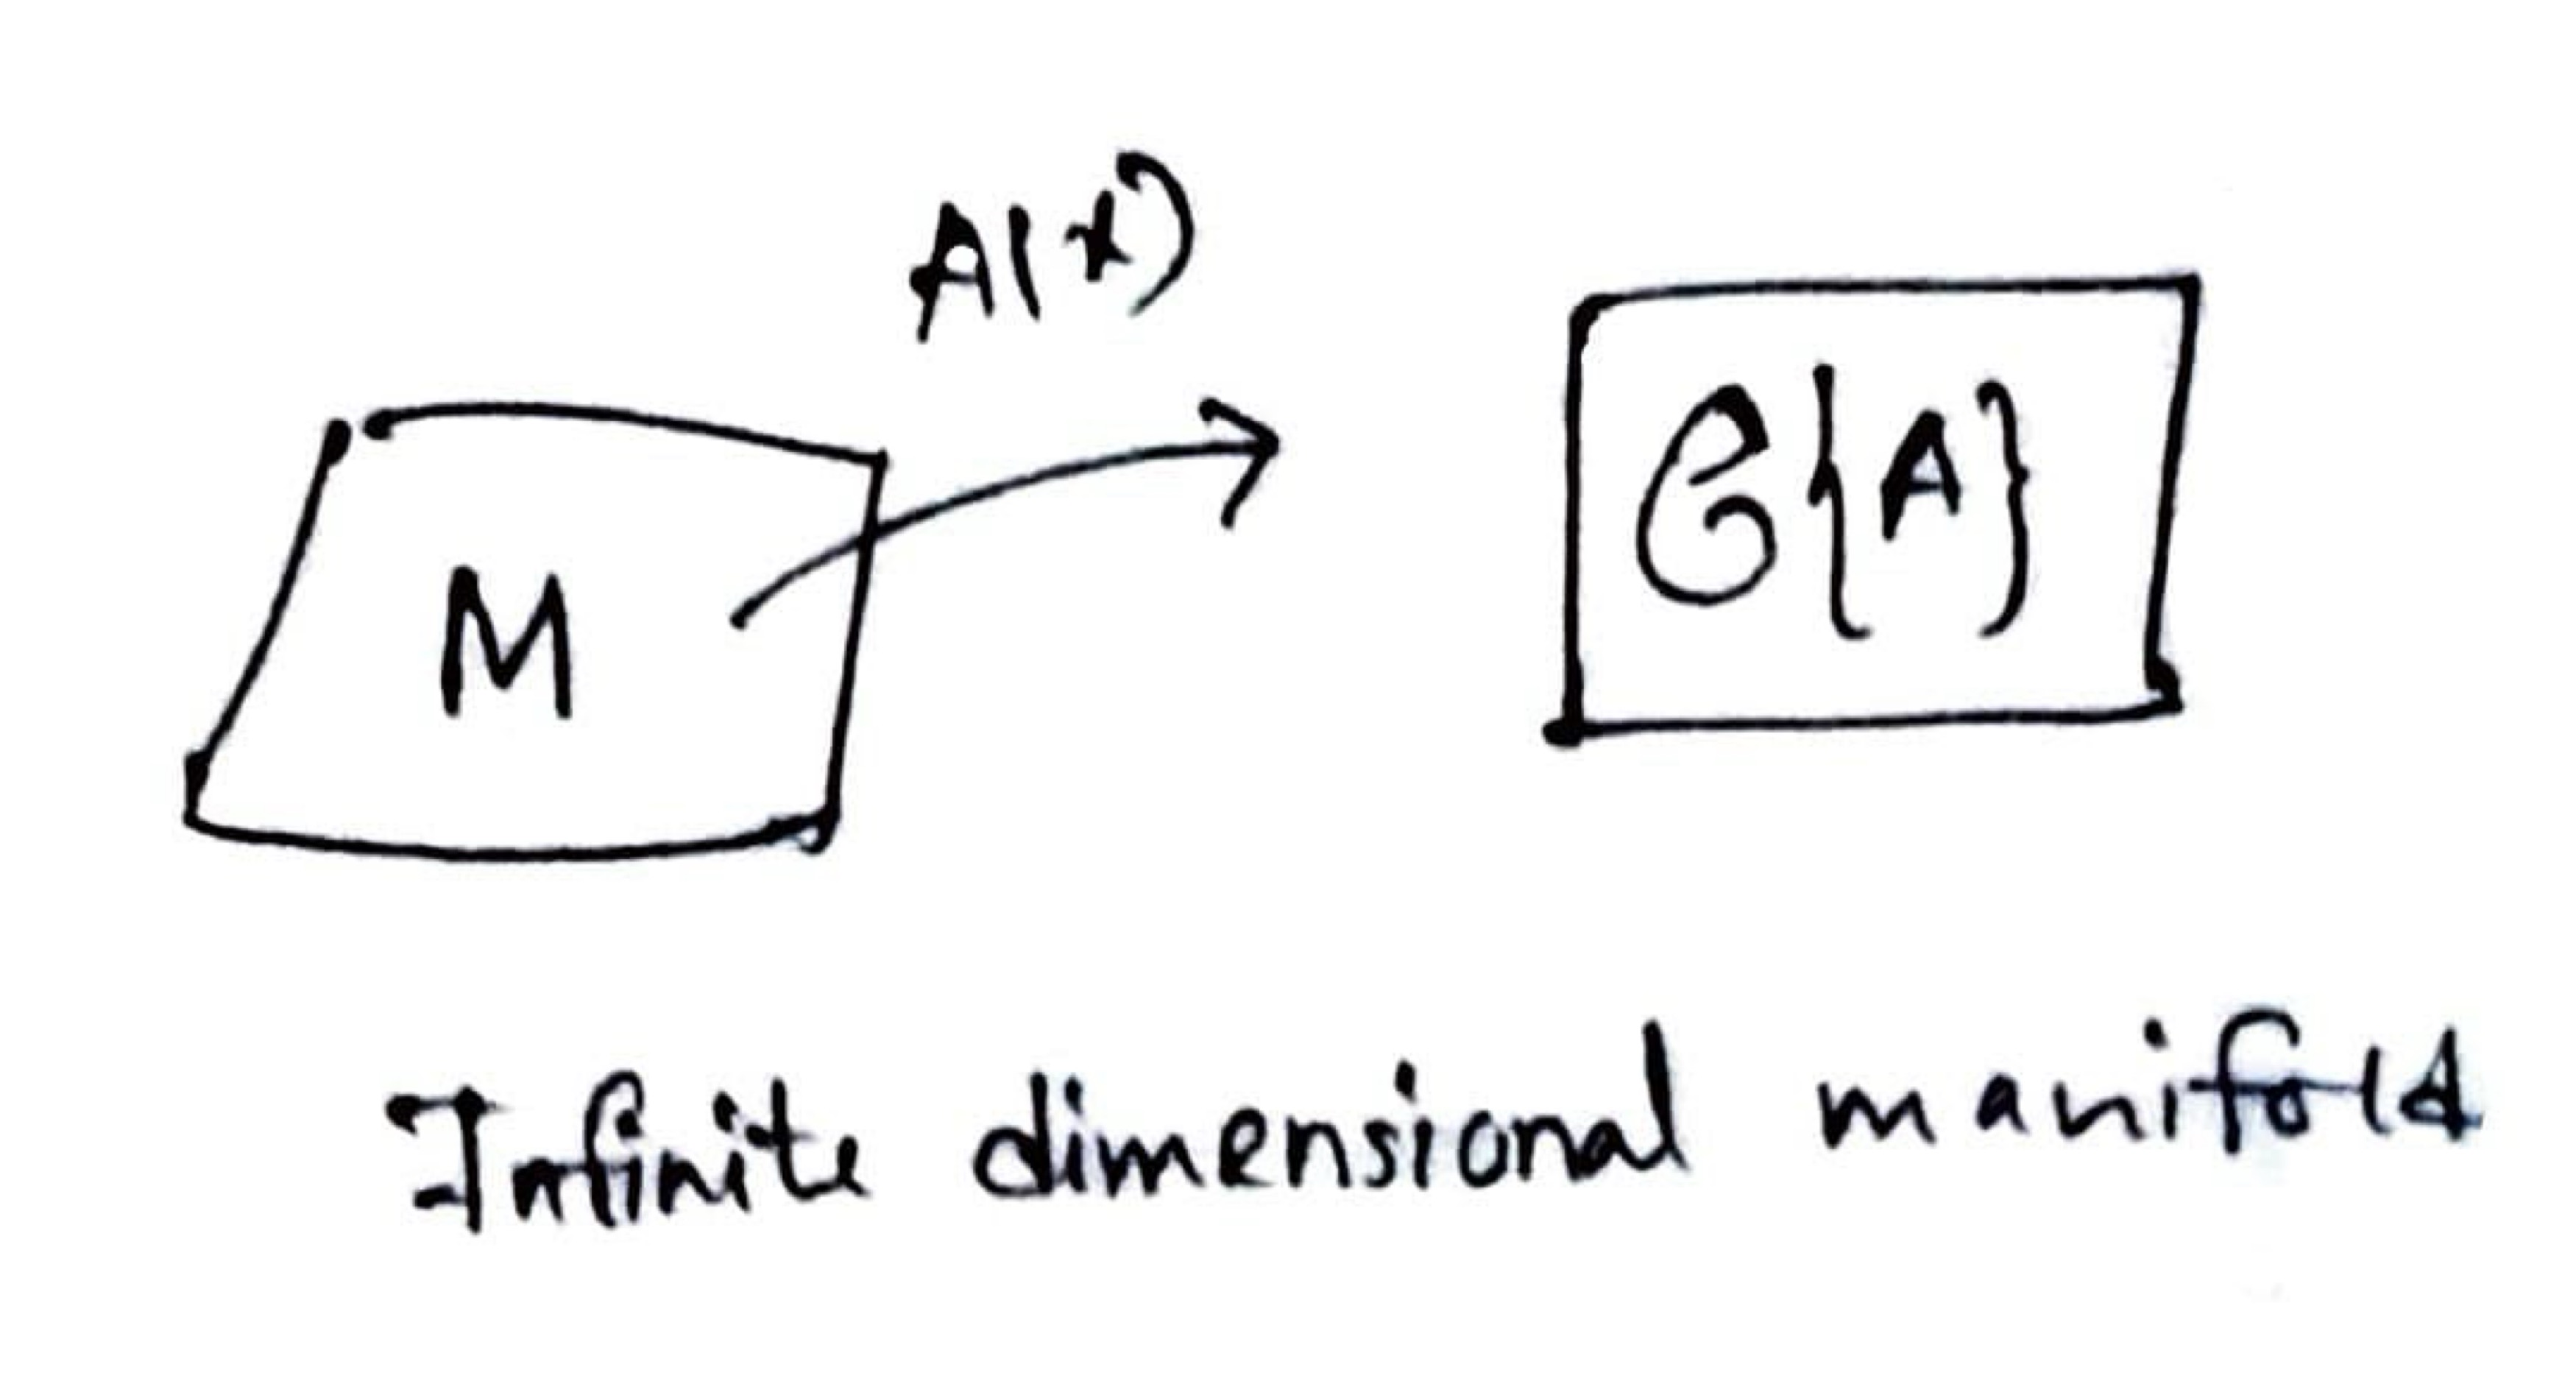
\includegraphics[width=0.4\linewidth]{figures/C09_2.jpeg}
    \caption*{}
\end{figure}
\vspace{-1cm}
\begin{tcolorbox}[title=Notes]
\begin{itemize}
    \item It's like a translation in internal space.
    \item Translation of a configuration space.
    \item Transformation is thought as a translation in extra dimension.
\end{itemize}
\end{tcolorbox}
Now, we want the action (Lagrangian) to be invariant under gauge transformation \eqref{9.2}.
\begin{align*}
-J_b A^b &\to -J_b (A^b + \partial^b F) \\
&= -J_b \, A^b - J_b \,\partial^b F \\
&= -J_b \, A^b +(\partial^b J_b) F \quad [ \text{integration by parts} ]
\end{align*}
\begin{itemize}
    \item $F$ must vanish on boundaries
    \item $F$ is not arbitrary.
    \item Therefore the current must be conserved.
\end{itemize}
\[
\therefore ~\partial^b J_b = 0 \quad; \quad \text{for all } J
\]
\begin{itemize}
    \item Classical EOM $\neq$ Whole Configuration Space.
    \item Here, we extremize action.
\end{itemize}

\subsection{Covariant Derivative}
\begin{figure}[H]
    \centering
    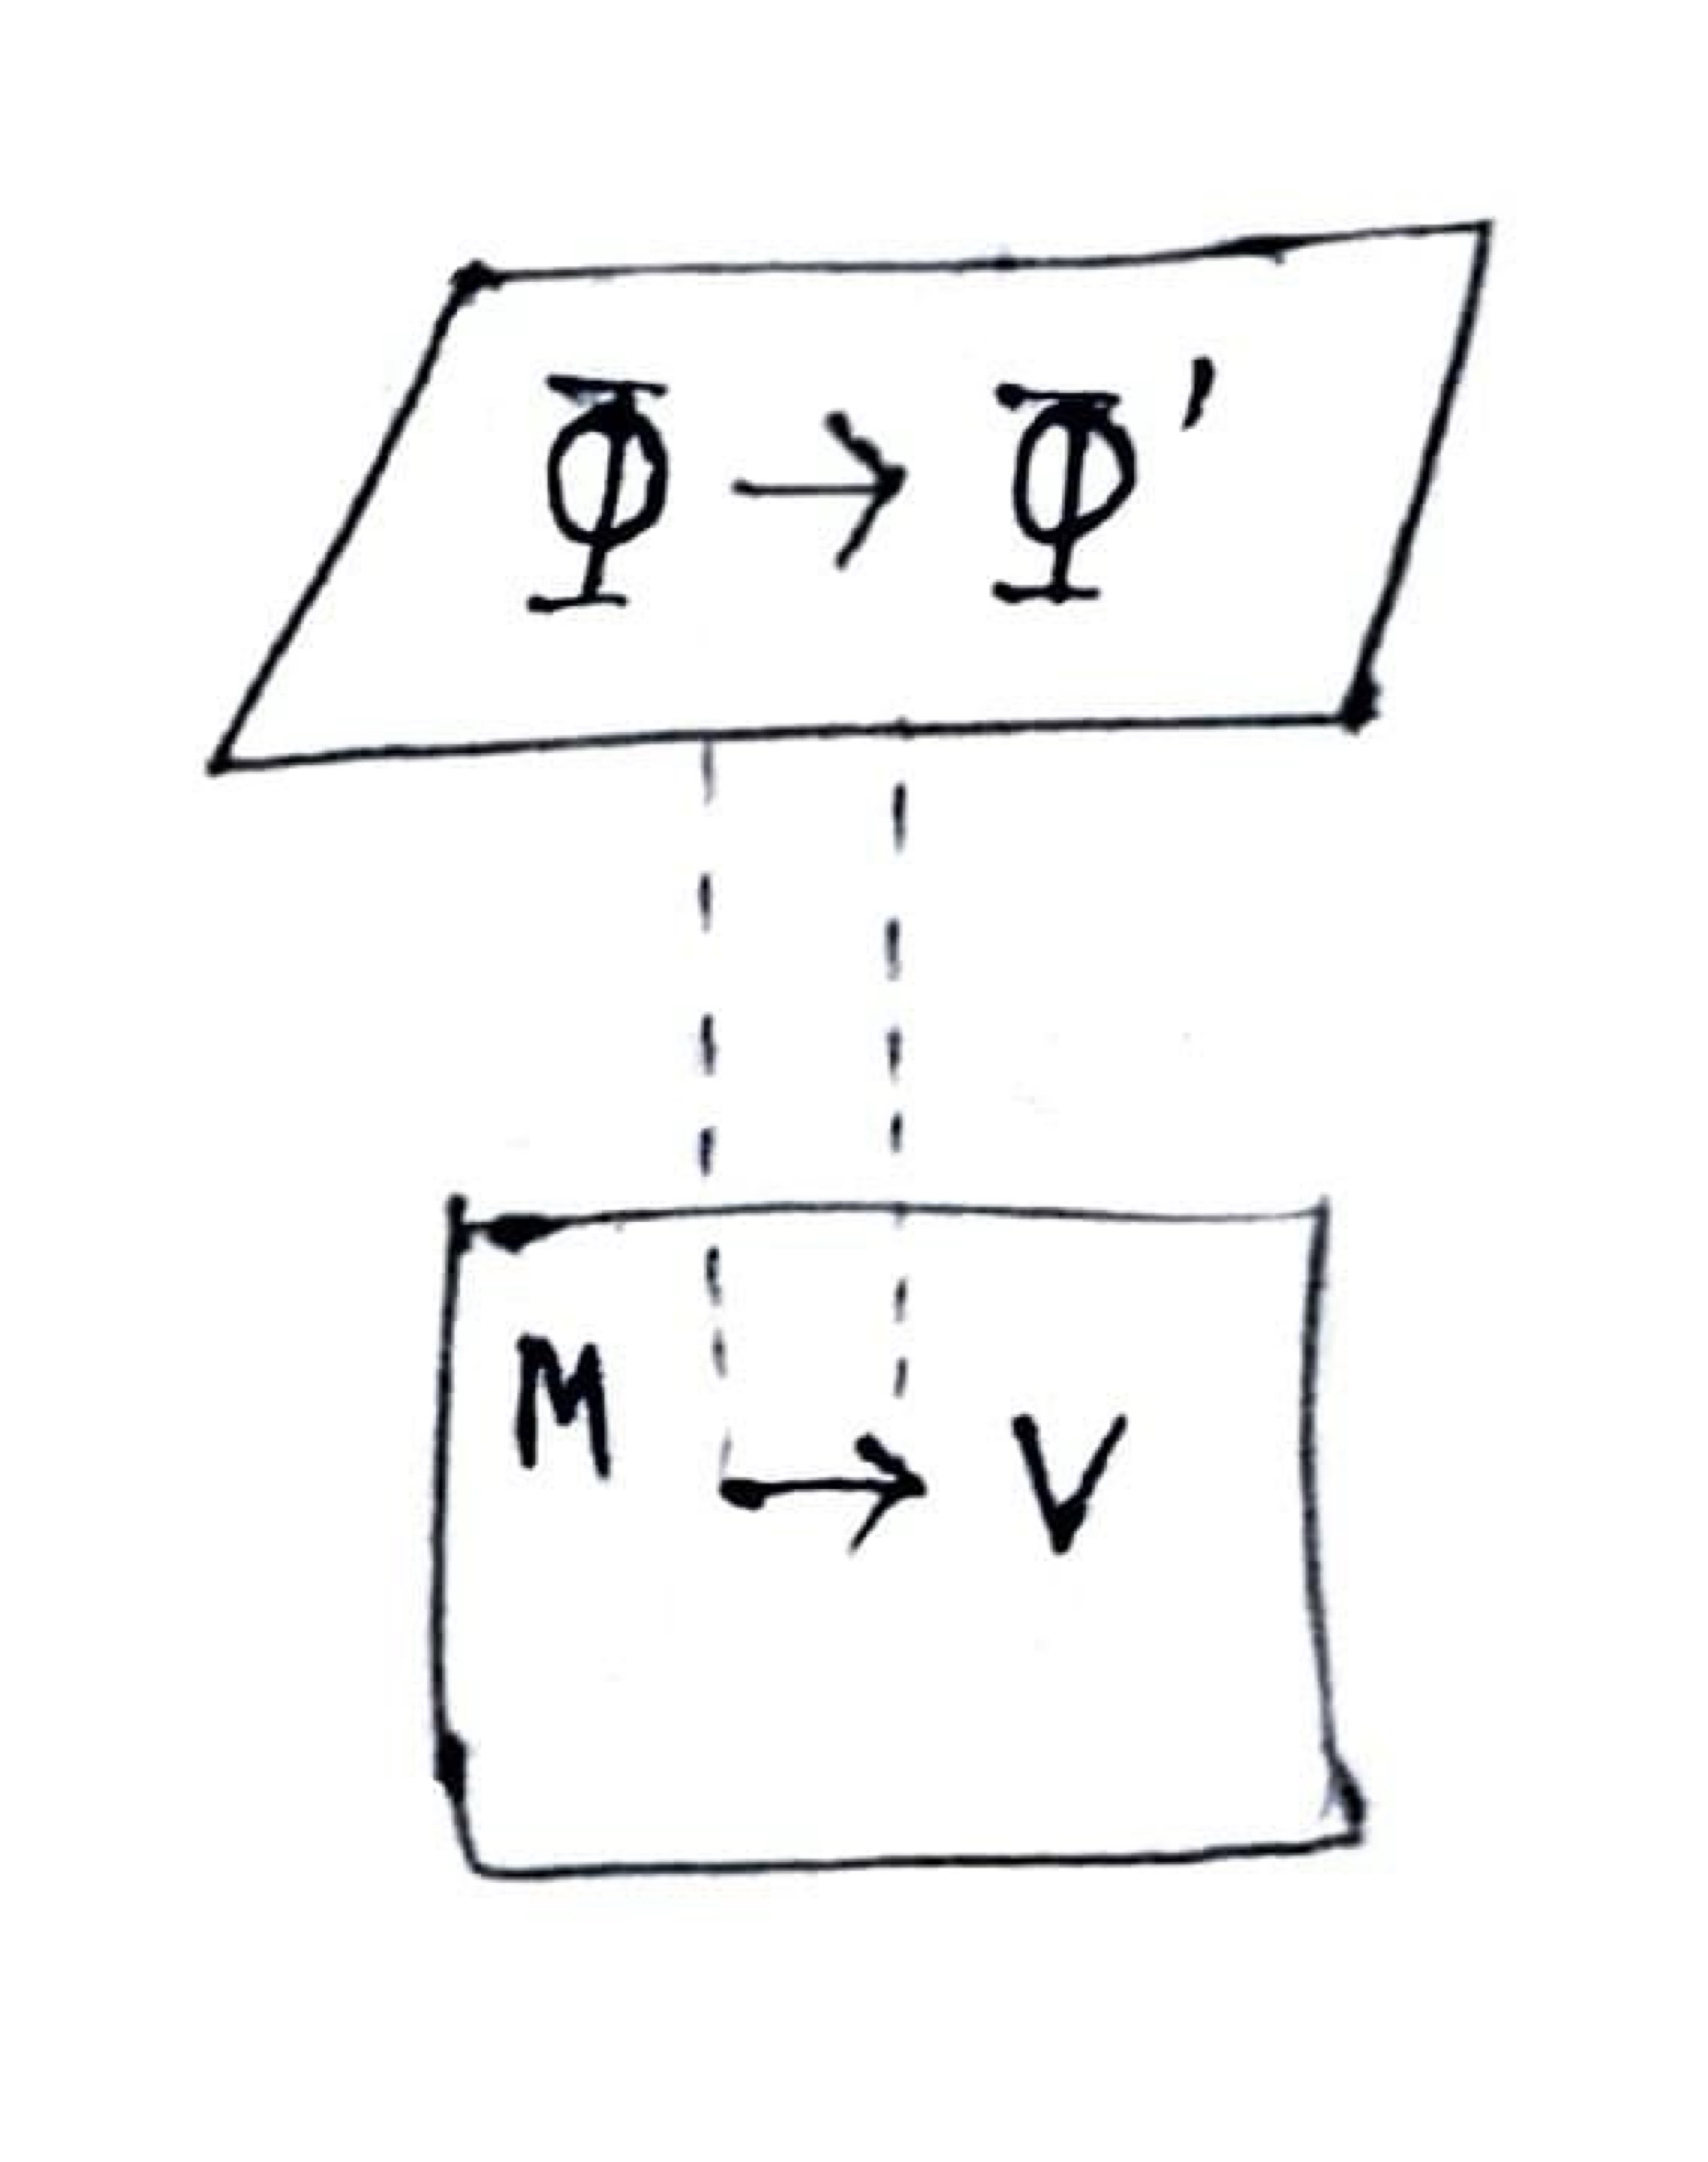
\includegraphics[width=0.3\linewidth]{figures/C09_3.jpeg}
    \caption*{}
\end{figure}
\vspace{-1.5cm}
\[
\phi \rightarrow \phi' = M \phi \quad; \quad M = M(x)
\]
\[
\partial_\mu \phi \to  \partial_\mu \phi' =\partial_\mu (M \phi) = M \partial_\mu \phi + (\partial_\mu M) \phi
\]
The latter term $(\partial_\mu M) \phi$ denotes there is another space dependency on $\phi$

$M$ is a matrix valued. Now we have to add terms whose linear addition removes this garbage (extra term). Therefore,
\[
D_\mu \phi \to M D_\mu \phi \equiv D'_\mu \phi' \equiv D'_\mu (M \phi)
\]
\begin{tcolorbox}
Derivative is not hermitian, it is anti-hermitian. Hence we write,
\[
D_\mu \phi = \partial_\mu \phi + i A_\mu \phi \quad \text{instead of} \quad \partial_\mu \phi + A_\mu \phi.
\]
Also $D_\mu$ is an associative operation.
\end{tcolorbox}

\begin{align*}
&\quad \quad \quad D_\mu'b = M ~D_\mu ~ M^{-1} \\
&\Rightarrow (\partial_\mu + i A'_\mu) = M (\partial_\mu + i A_\mu) M^{-1} \\
&\Rightarrow \partial_\mu + i A'_\mu = \partial_\mu + i ~M A_\mu M^{-1} \quad [\because M \partial_\mu M^{-1} = \partial_\mu]\\
&\Rightarrow i A'_\mu = M (\partial_\mu M^{-1}) + i~ M A_\mu M^{-1}\\
&\Rightarrow i A'_\mu = M \partial_\mu M^{-1} + i ~M A_\mu M^{-1} \\
&\therefore ~~~ A'_\mu = M A_\mu M^{-1} - i ~M \partial_\mu M^{-1}
\end{align*}

\textbf{Findings:}
\begin{itemize}
\item $D$ is matrix valued.
\item $D_\mu$ transforms covariantly $\to$ Tensor
\item $A_\mu$ doesn't transform covariently $\to$ Tensor
\end{itemize}
Now,
\begin{align*}
\tilde{F}_{\mu \nu} &= \frac{1}{i} [D_\mu, D_\nu] \\
&= \frac{1}{i}\big[\partial_\mu \mathbb{I}+ i A_\mu ~,~ \partial_\nu \mathbb{I}+ i A_\nu  \big] \\
&= \frac{1}{i}\left\{ i \big[ \mathbb{I} \partial_\mu , A_\nu \big] + i\big[ A_{\mu}, \mathbb{I} \partial_\nu\big]+i^2 \big[A_\mu , A_\nu \big] \right\} \quad \big( \because \big[ \partial_\mu , \partial_\nu \big] =0 \big)  \\
\therefore\tilde{F}_{\mu\nu} &= \partial_\mu A_\nu - \partial_\nu A_\mu + i[A_\mu, A_\nu] \\
\therefore [D_\mu, &D_\nu] \text{ is a curvature}
\end{align*}
% $A, B$ are hermitian, so
% \[
% [A, B] \text{ is antihermitian}
% \]
Now,
\begin{align*}
\tilde{F}_{\mu \nu} &= M \,F_{\mu \nu} \, M^{-1} \\
&= -\frac{1}{i} \big[D_\mu, D_\nu \big] \\
&= -\frac{1}{i} \left[ M \,D_\mu \,M^{-1}, M \, D_\nu \, M^{-1} \right] \\
&= -\frac{1}{i} M \big[D_\mu, D_\nu \big] M^{-1} \\
\therefore \tilde{F}_{\mu \nu}&= M \,\tilde{F}_{\mu \nu}\, M^{-1}
\end{align*}
Now, for a transformation $\quad \phi \to \phi' = M \phi$
\begin{align*}
A_\mu \to M A_\mu M^{-1} - i \,M \partial_\mu M^{-1} \quad \tag{9.3a} \label{9.3a} \\
\bar{A}_\mu \to M \bar{A}_\mu M^{-1} - i\,M \partial_\mu M^{-1} \quad \tag{9.3b} \label{9.3b}
\end{align*}
Subtracting \eqref{9.3b} to \eqref{9.3a} we get
\[
(\bar{A}_\mu - A_\mu) \to M\,(\bar{A}_\mu - A_\mu) \, M^{-1}
\]
Therefore, the variation $(\bar{A}_\mu - A_\mu)$ of a connection acts as a tensor, not $A_\mu$ itself.
\begin{tcolorbox}[ title=Extra information]
\begin{itemize}
\item [a)] \textbf{Affine space}: the origin is not known.
\item [b)] If $A$ is a matrix, we can define some norm out of it:
    \begin{itemize}
        \item $\det A \to$ not additive
        \item Tr $A \to$ additive
    \end{itemize}
\end{itemize}
\end{tcolorbox}
Now,
\begin{align*}
S_{YM} &= -\frac{1}{4} \int d^D x \, \mathrm{Tr}\left( \tilde{F}_{\mu \nu} \tilde{F}^{\mu \nu} \right) \\
\delta S_{YM} &= -\frac{1}{2} \int d^D x \, \mathrm{Tr}\left( \tilde{F}^{\mu \nu} \delta \tilde{F}_{\mu \nu} \right) =0 \tag{9.4} \label{9.4}
\end{align*}
Here,
\begin{align*}
\delta \tilde{F}_{\mu \nu} &= \frac{1}{i}\, \delta [D_\mu, D_\nu] \\
&= \frac{1}{i} \delta (D_\mu D_\nu - D_\nu D_\mu) \\
&= \frac{1}{i} \left\{ (\delta D_\mu) D_\nu + D_\mu (\delta D_\nu) - (\delta D_\nu) D_\mu - D_\nu (\delta D_\mu) \right\} \\
&= -\frac{1}{i} \left\{ [\delta D_\mu, D_\nu] + [D_\mu, \delta D_\nu] \right\} \\
&=[\delta A_\mu, D_\nu] + [D_\mu, \delta A_\nu] \\
\therefore \delta \tilde{F}_{\mu \nu} &= [D_\mu, \delta A_\nu] - [D_\nu, \delta A_\mu] \tag{9.5} \label{9.5}
\end{align*}
\begin{tcolorbox}
Recall for electromagnetism,
\[
\delta F_{\mu \nu} = \partial_\mu (\delta A_\nu )-\partial_\nu (\delta A_\mu) = [\partial_\mu , \delta A_\nu ] - [\partial_\nu , \delta A_\mu]
\]
\end{tcolorbox}
Using \eqref{9.5} in \eqref{9.4} we get,
\begin{align*}
\delta S_{YM} &= -\frac{1}{2} \int d^D x \, \mathrm{Tr}\left( \tilde{F}^{\mu \nu}\left\{ \big[ D_\mu, \delta A_\nu \big] - \left[ D_\nu, \delta A_\mu \right] \right\}\right) \\
&= -\frac{1}{2} \int d^D x \, \mathrm{Tr}\left( \tilde{F}^{\mu \nu}\left[ D_\mu, \delta A_\nu \right] - \tilde{F}^{\mu \nu}\left[ D_\nu, \delta A_\mu \right] \right) \\
&=- \int d^D x \, \mathrm{Tr}\left( \tilde{F}^{\mu \nu}\left[ D_\mu, \delta A_\nu \right]\right) \\
\therefore \delta S_{YM}&= \int d^D x \, \mathrm{Tr}\left( \left[ D_\mu, \tilde{F}^{\mu \nu}\right] \delta A_\nu \right) = 0
\end{align*}
\[
\therefore \left[ D_\mu, F^{\mu \nu}\right]=0 \quad (\tilde{F}_{\mu \nu} \to A^1 + A^2 \to A^3 \quad \text{highly nonlinear})
\]
\begin{tcolorbox}
Proof of \eqref{9.5},
\[
\mathrm{Tr}\big( A[X,B] \big) = - \mathrm{Tr}\big([X,A]B \big)  
\]
\begin{align*}
\mathrm{Tr}\big( A[X,B] \big) &= \mathrm{Tr}\big( AXB - ABX \big) \\
&= \mathrm{Tr}\big( XAB \big) + \mathrm{Tr}\big( AXB \big) \\
&= -\mathrm{Tr}\big( ~\{XA-AX\} B ~\big) \\
\therefore \mathrm{Tr}\big( A[X,B] \big)&= - \mathrm{Tr}\big( [X,A]B \big) \\
\therefore \mathrm{Tr}\big( \tilde{F}_{\mu \nu}[D_\mu,\delta A_\nu] \big)&= - \mathrm{Tr}\big( [D_\mu,\tilde{F}_{\mu \nu}] \delta A_\nu \big)
\end{align*}
\end{tcolorbox}

\newpage

\stepcounter{section}
\renewcommand{\thesection}{\arabic{section}}
\fancysection{(\textit{\textbf{Class-10})} Lecture \textbf{7}: Sat, July 5, 2025}{\textbf{\textit{Path Integral Formalism}}}
%---
\subsection{Quantization}
\subsubsection{What is Quantization?}
Quantization is the process that turns classical variables into quantum operators that act on a state space. 
\newline
\textbf{Example:} In the harmonic oscillator, we quantize by defining:
\begin{itemize}
    \item Ladder operators: \( a, a^\dagger \)
    \item Number states: \( \ket{n} \)
\end{itemize}

Then, we can calculate overlaps like:
\[
\bra{m} e^{i\hat{H}t/\hbar} \ket{n}
\]
\begin{tcolorbox}[ title=Overlaps]
In quantum mechanics, states are represented as vectors in a Hilbert space. The overlap between two quantum states \( \ket{\psi} \) and \( \ket{\phi} \) is their inner product:
\[
\braket{\phi|\psi} \quad \text{(Complex number)}
\]
\end{tcolorbox}
This is only possible because we quantized—i.e., built a Hilbert space of states and defined how operators act.
\[
\boxed{\textbf{No Hilbert Space = No quantization.}}
\]

\subsubsection{Why Quantization?}
\begin{itemize}
    \item Matches with experimental results.
    \item The ultimate goal is to calculate \textbf{overlaps}. No operators / Hilbert space is necessarily involved.
\end{itemize}
\vspace{1cm}
\begin{tcolorbox}[ title=Note]
\subsubsection*{Why in quantum mechanics we take \( [a, a^\dagger] = 1 \)but why not \( a^\dagger \ket{0} = 0 \)?}
Because if \( a^\dagger \ket{0} = 0 \), then:
\[
(x + ip) \psi = 0 \quad \Rightarrow \quad \left( x - \frac{d}{dx} \right) \psi = 0
\]
If \( \psi \sim A e^{+x^2/2} \), it won't be normalizable.
\end{tcolorbox}
\subsection{Quantization Methods}
\begin{figure}[H]
    \centering
    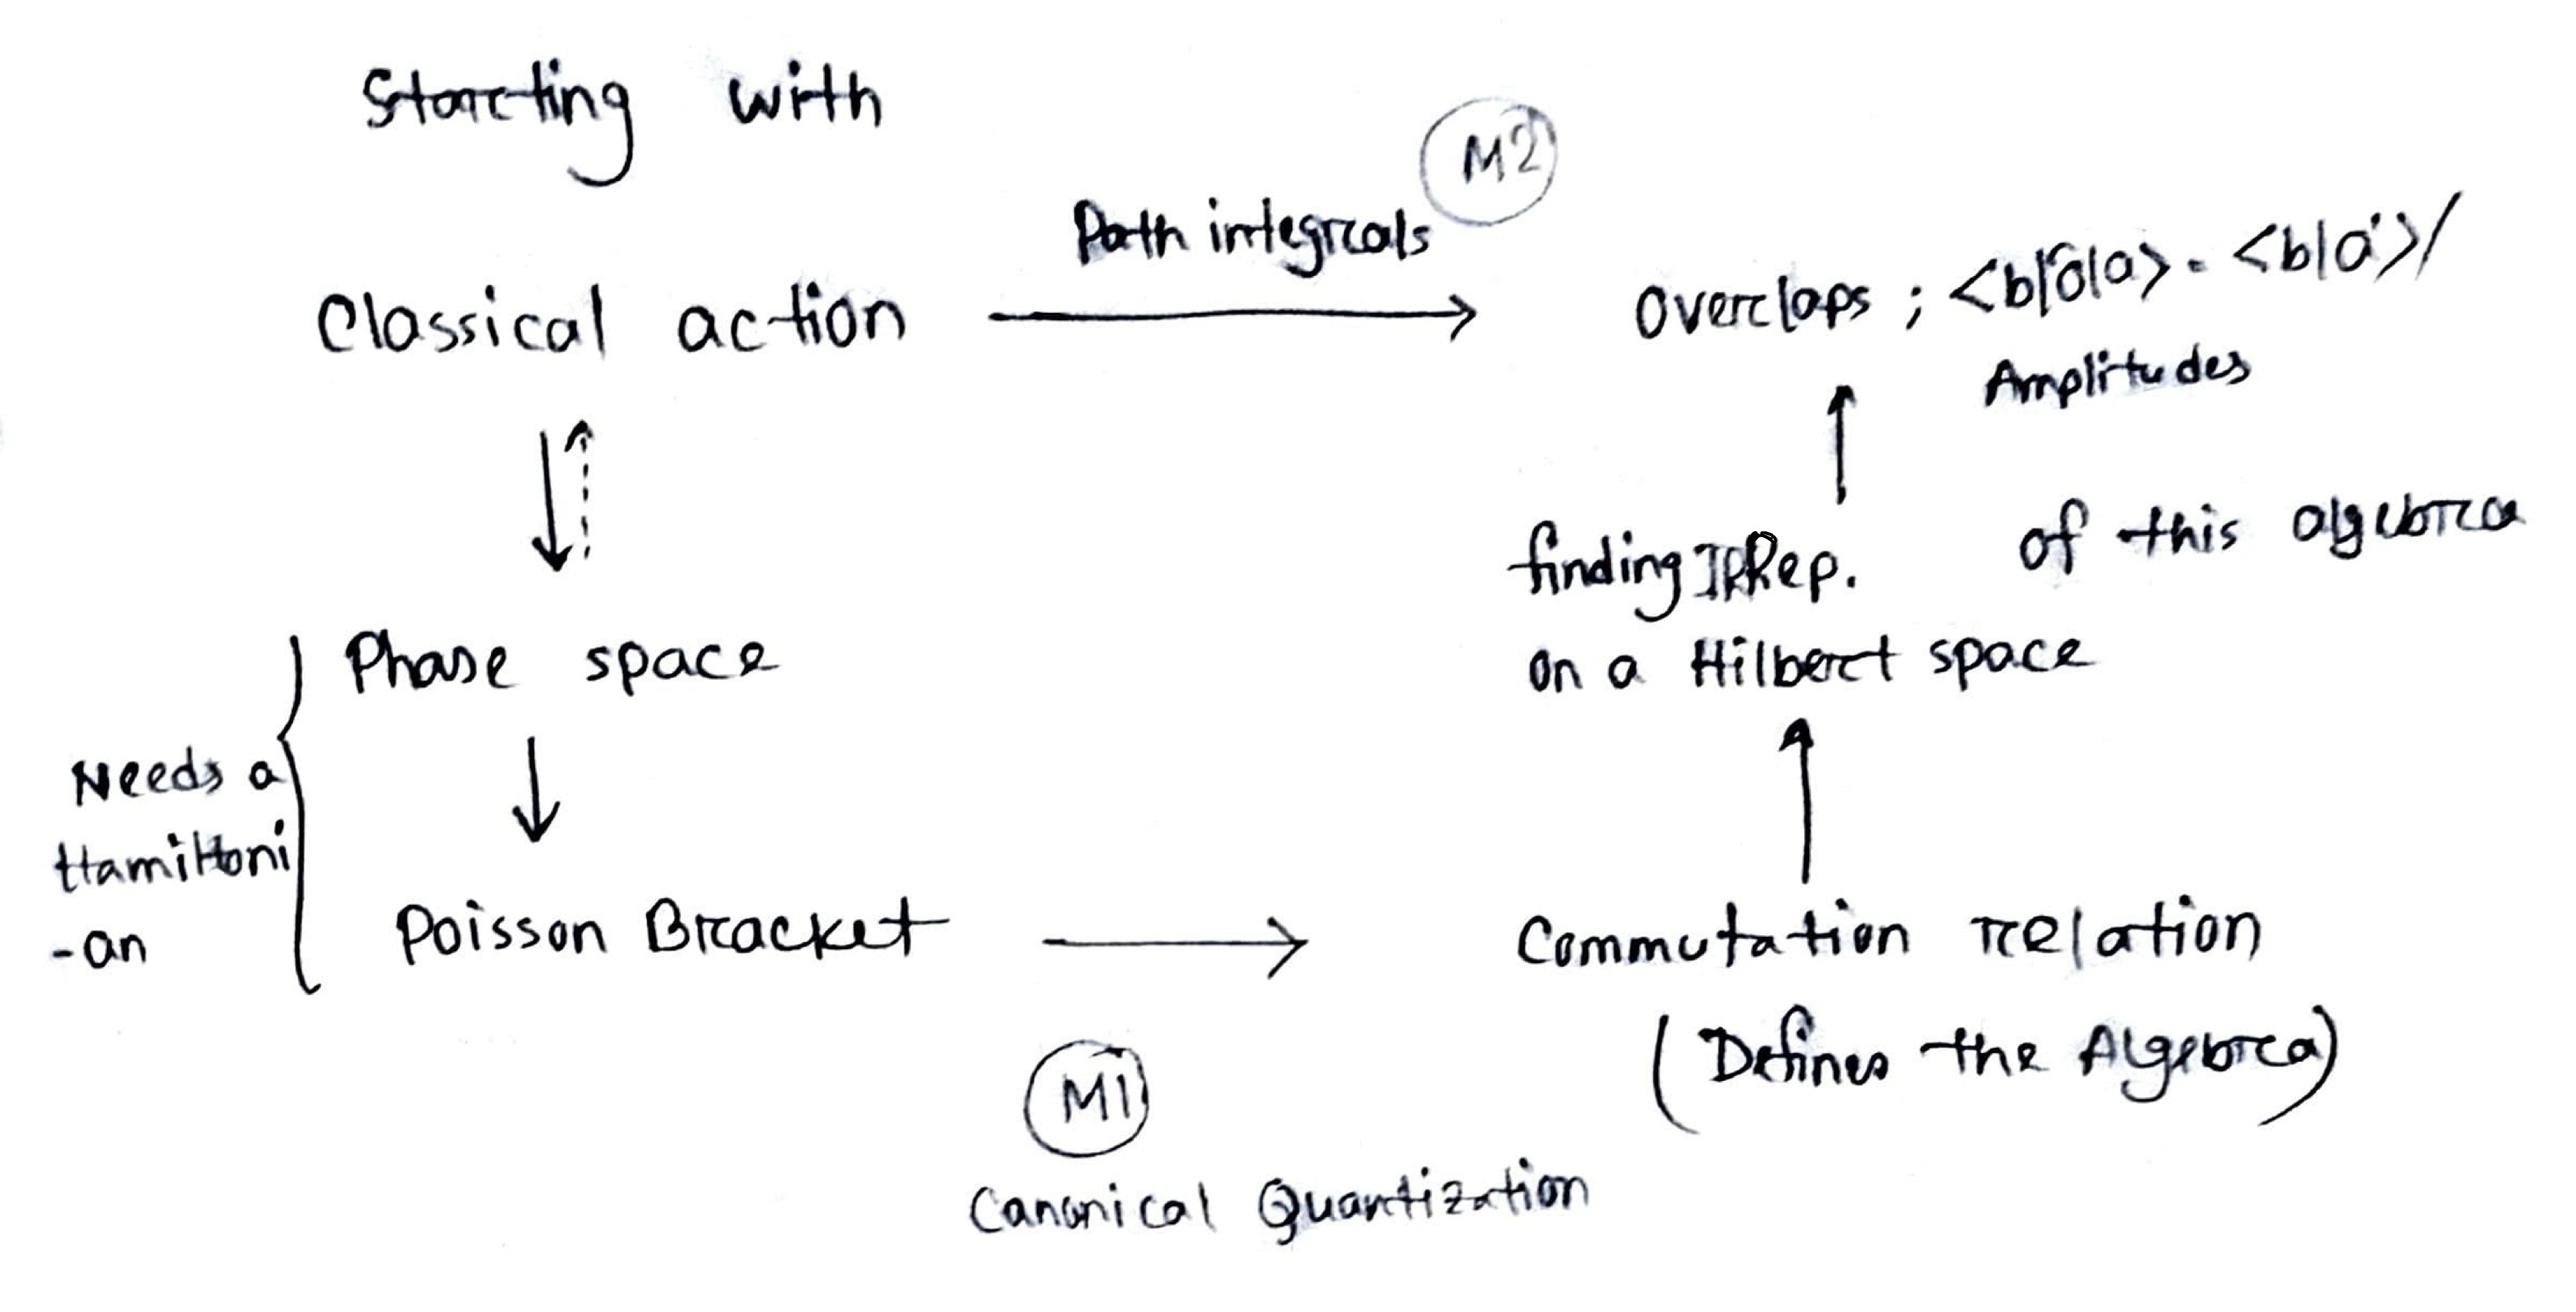
\includegraphics[width=1.1\linewidth]{figures/C10_1.jpeg}
    \caption*{}
\end{figure}
% \vspace{}
% Starting with classical action:

% \[
% \text{Classical Action} \longrightarrow \text{Phase Space} \longrightarrow \text{Poisson Bracket} \longrightarrow \text{Commutation Relation}
% \]

% \begin{itemize}
%     \item[\textbf{M1}] Canonical Quantization
%     \item[\textbf{M2}] Path Integrals
% \end{itemize}

% \textbf{Overlaps:} \( \braket{\phi | O | \psi} \) = Amplitude of observation

\begin{tcolorbox}
\subsection*{GNS Construction}
\[\text{GNS Construction : Algebra} \rightarrow \text{Hilbert space} \]
Regular Representation of a Group (Algebra):
\[
gg' = g' g
\]
Think of a vector:
\[
R(g)
\begin{pmatrix}
g_1 \\
g_2 \\
\vdots \\
g_n
\end{pmatrix}
=
\begin{pmatrix}
g_1' \\
g_2' \\
\vdots \\
g_n'
\end{pmatrix}
\]
\begin{itemize}
    \item Regular representation is not necessarily an irreducible representation (irrep).
\end{itemize}

\subsection*{Adjoint Representation}
\[
\big[T(g), g\big] = g''
\]
\begin{itemize}
    \item Adjoint Rep. is an irrep.
\end{itemize}
Also,
\[Algebra \to \text{existence of a cyclic vector} \equiv \text{choice of a vacuum state}
\]
\end{tcolorbox}

\section*{Back to Hamiltonian Formulation}
The Hamiltonian depends on a choice of coordinates. It's not a covariant concept.

\begin{enumerate}
    \item We find \( H \) from conjugate momenta.
    \item Then need Lagrangian \( \mathcal{L} \)
    \item Then need \textbf{dot} i.e., time derivatives
    \item Which is frame dependent
    \item Proper time needs to be defined
\end{enumerate}
Hence, not good from the vantage point of General Relativity.
\begin{tcolorbox}
\subsection*{Haag's Theorem}
\textbf{Statement:} The interaction picture does not rigorously exist in interacting relativistic quantum field theory.
\end{tcolorbox}
\subsection{Pictures in Quantum Mechanics}
\begin{center}
\begin{tabular}{@{}lccc@{}}
\toprule
Pictures    & State & Operator \\
\midrule
Schrödinger & \checkmark & $\times$ \\
Heisenberg  & $\times$   & \checkmark \\
\bottomrule
\end{tabular}
\end{center}
\[
\text{QFT} \to  \text{Infinite Degrees of Freedom}
\]
\textbf{Schrödinger Picture:} Needs a state vector which is a \textbf{functional} of the degrees of freedom (DOFs).

In one particle,
\begin{itemize}
    \item \( \hat{x} \to \) can be independent of time
    \item \( \psi \to \) can be time dependent
\end{itemize}
$\therefore \, \hat{x} \ket{\psi} \to$ eigenvalue can be dependent on time.
\begin{tcolorbox}
In Quantum Field Theory, 
\[
\psi (x) \to \psi [\phi]
\]
This is because $x$ is just a \textbf{label}, so relabeling does not change the wavefunction.
\end{tcolorbox}
\noindent
Also for one particle,
\[\psi \sim e^{-x^2/2}\]
But for many particles,
\[\psi \sim e^{-x_1^2/2} ~\cdot e^{-x_2^2/2} \dots \dotsc \sim \prod_i e^{-x_i^2/2} \]
\begin{figure}[H]
    \centering
    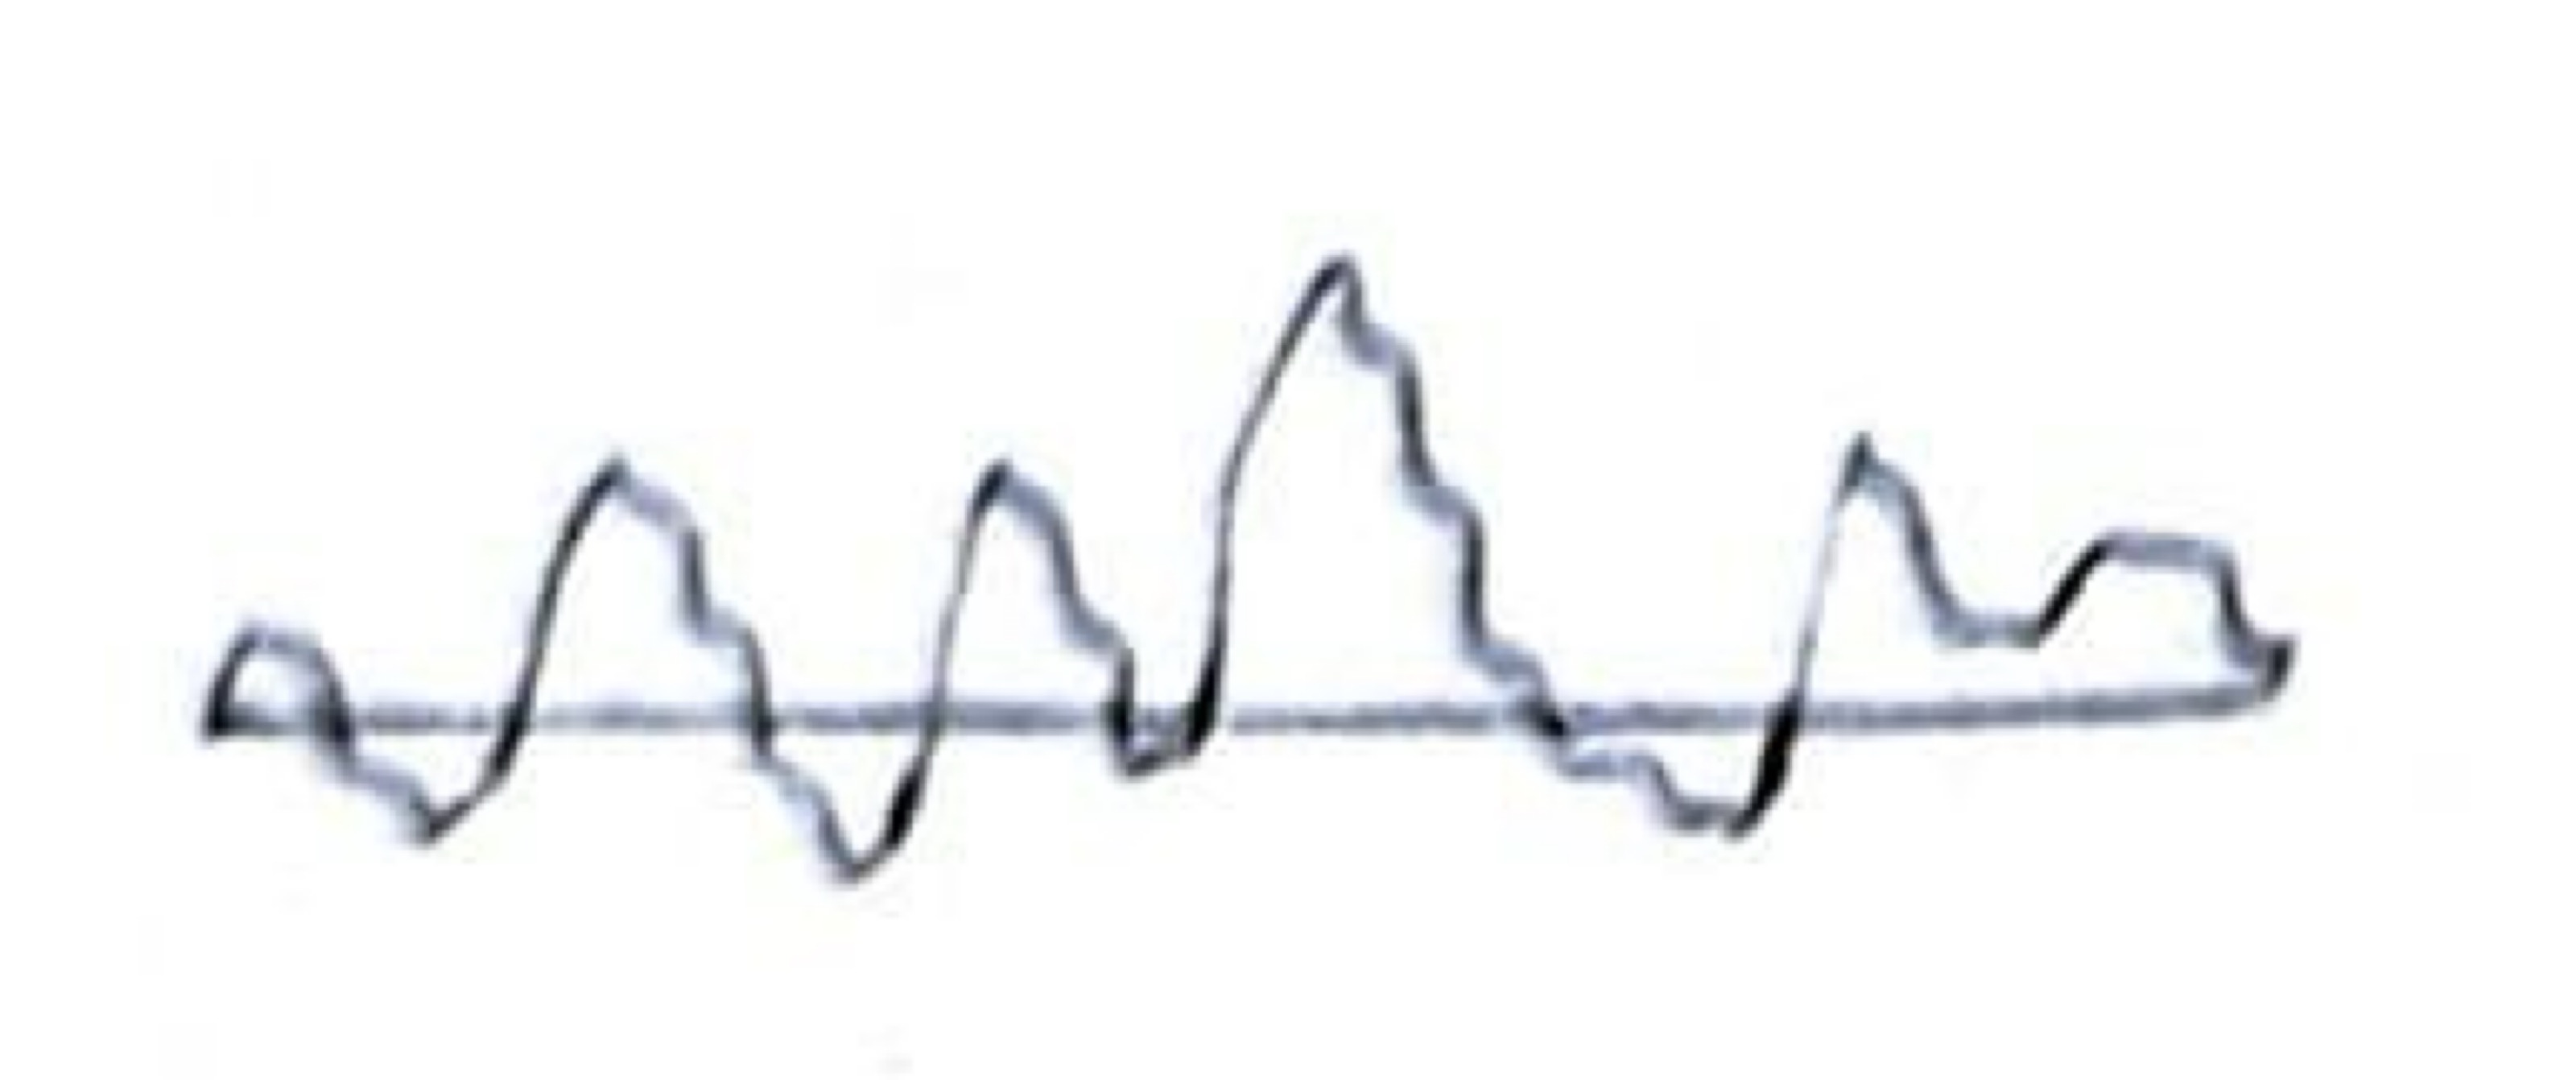
\includegraphics[width=0.4\linewidth]{figures/C10_3.jpeg}
    \caption*{}
\end{figure}
% \vspace{}
For Hamiltonian:
\[
H = \sum_i p_i^2 + V = -\sum_i \left(\frac{\partial^2}{\partial x_i^2}\right) + V
\]
As we can see there are infinite derivatives $\big(\frac{\partial}{\partial x}\big)$ and we need to find their eigenvalues. This is why the Heisenberg picture is often preferred where, \textbf{states are independent of time}. 

\begin{tcolorbox}
\textbf{Notice, in Quantum Mechanics:}
\[
[x_i, p_j] = i \hbar \delta_{ij}
\]
- Eigenvalues are unbounded  
- \(1 \leq i,j \leq \mathbb{N}\)  
- Degrees of freedom are \textbf{finite} \\[1em]

\textbf{In Quantum Field Theory:}
\[
[\phi(x), \pi(y)] = i\, \delta^3(x - y)\, \hat{\mathbb{I}}
\]
- Degrees of freedom are \textbf{infinite}  
- Representations of the commutation relations are \textbf{not unitarily equivalent} \\[1em]

\textbf{Another way to realize this:}
\[
[x_i, p_j] = i \hbar \delta_{ij}
\]
The trace of the right-hand side is non-zero:  
\[
\mathrm{Tr}(\mathbb{I}) \neq 0
\]
But the trace of the left-hand side:
\[
\mathrm{Tr}(xp - px) =
\begin{cases}
0        & \text{(finite d.o.f.)} \\
\neq 0   & \text{(infinite d.o.f.)}
\end{cases}
\]
\end{tcolorbox}
\noindent
We use the Heisenberg picture,

\subsubsection*{Free Particle Wavefunction}

\begin{align*}
\psi(x,t) &= e^{i(kx - \omega t)} \\
          &= e^{\frac{i}{\hbar}(px - Et)} \\
          &= e^{\frac{i}{\hbar} \int (p \frac{dx}{dt} - E) \, dt} \\
          &= e^{\frac{i}{\hbar} \int \mathcal{L} \, dt} \\
          &= e^{\frac{i}{\hbar} S}
\end{align*}

Also,
\[
\psi(x,t) = \braket{x |\, \psi, t}_S = \braket{x,t\, | \psi}_H
\]

We are interested in this "kernel":
\[
\braket{x',t' \,|\, x,t}
\]

\textbf{Why This Kernel?}

We assume we are dealing with linear equations:
\[
\hat{L} \phi(x) = J(x)  \quad ; \quad \text{Effect} \rightarrow \text{Cause} \tag{10.1} \label{10.1}
\]

Recall Ohm's law:

\begin{align*}
J &= \sigma E \\
\Rightarrow J(x) &= \sigma(x) E(x) \quad \text{(Local, like Maxwell's equations)} \\
\text{But,} \quad V &= IR \quad \text{(Bilocal: Involves two points)}
\end{align*}

Inversion of \eqref{10.1} yields:
\[
\phi(x) = \int G(x, y) J(y) \, dy
\]

Where:

\begin{itemize}
    \item \( G(x,y) \): Green’s Function (Kernel)
    \item \( \hat{L} \, G(x, y) = \delta(x,y) \quad \) (not \( \delta(x-y) \))
\end{itemize}
Effect at point $x$ caused by a source of unit strength localized at point $y$. That is: 
$$\langle b | V | a \rangle$$
\vspace{0.5cm}

\textbf{Important Notes:}
\begin{itemize}
    \item \( \delta(x, y) \rightarrow \) Localized cause
    \item \( G(x, y) \) is not necessarily symmetric
    \item Operator \( \hat{L} \) possesses translation symmetry
\end{itemize}
\begin{tcolorbox}
Checking \eqref{10.1}:
\begin{align*}
    \hat{L} \phi(x) &= \int \hat{L}\,G (x,y) J(y) \, dy \\
    &= \int \delta(x,y) J(y) \, dy \\
    &= J(x) \\
    \therefore \phi(x) &= \int G(x,y) J(y) \, dy
\end{align*}
\end{tcolorbox}

\subsection{Double Slit}
\vspace{-1.5cm}
\begin{figure}[H]
    \centering
    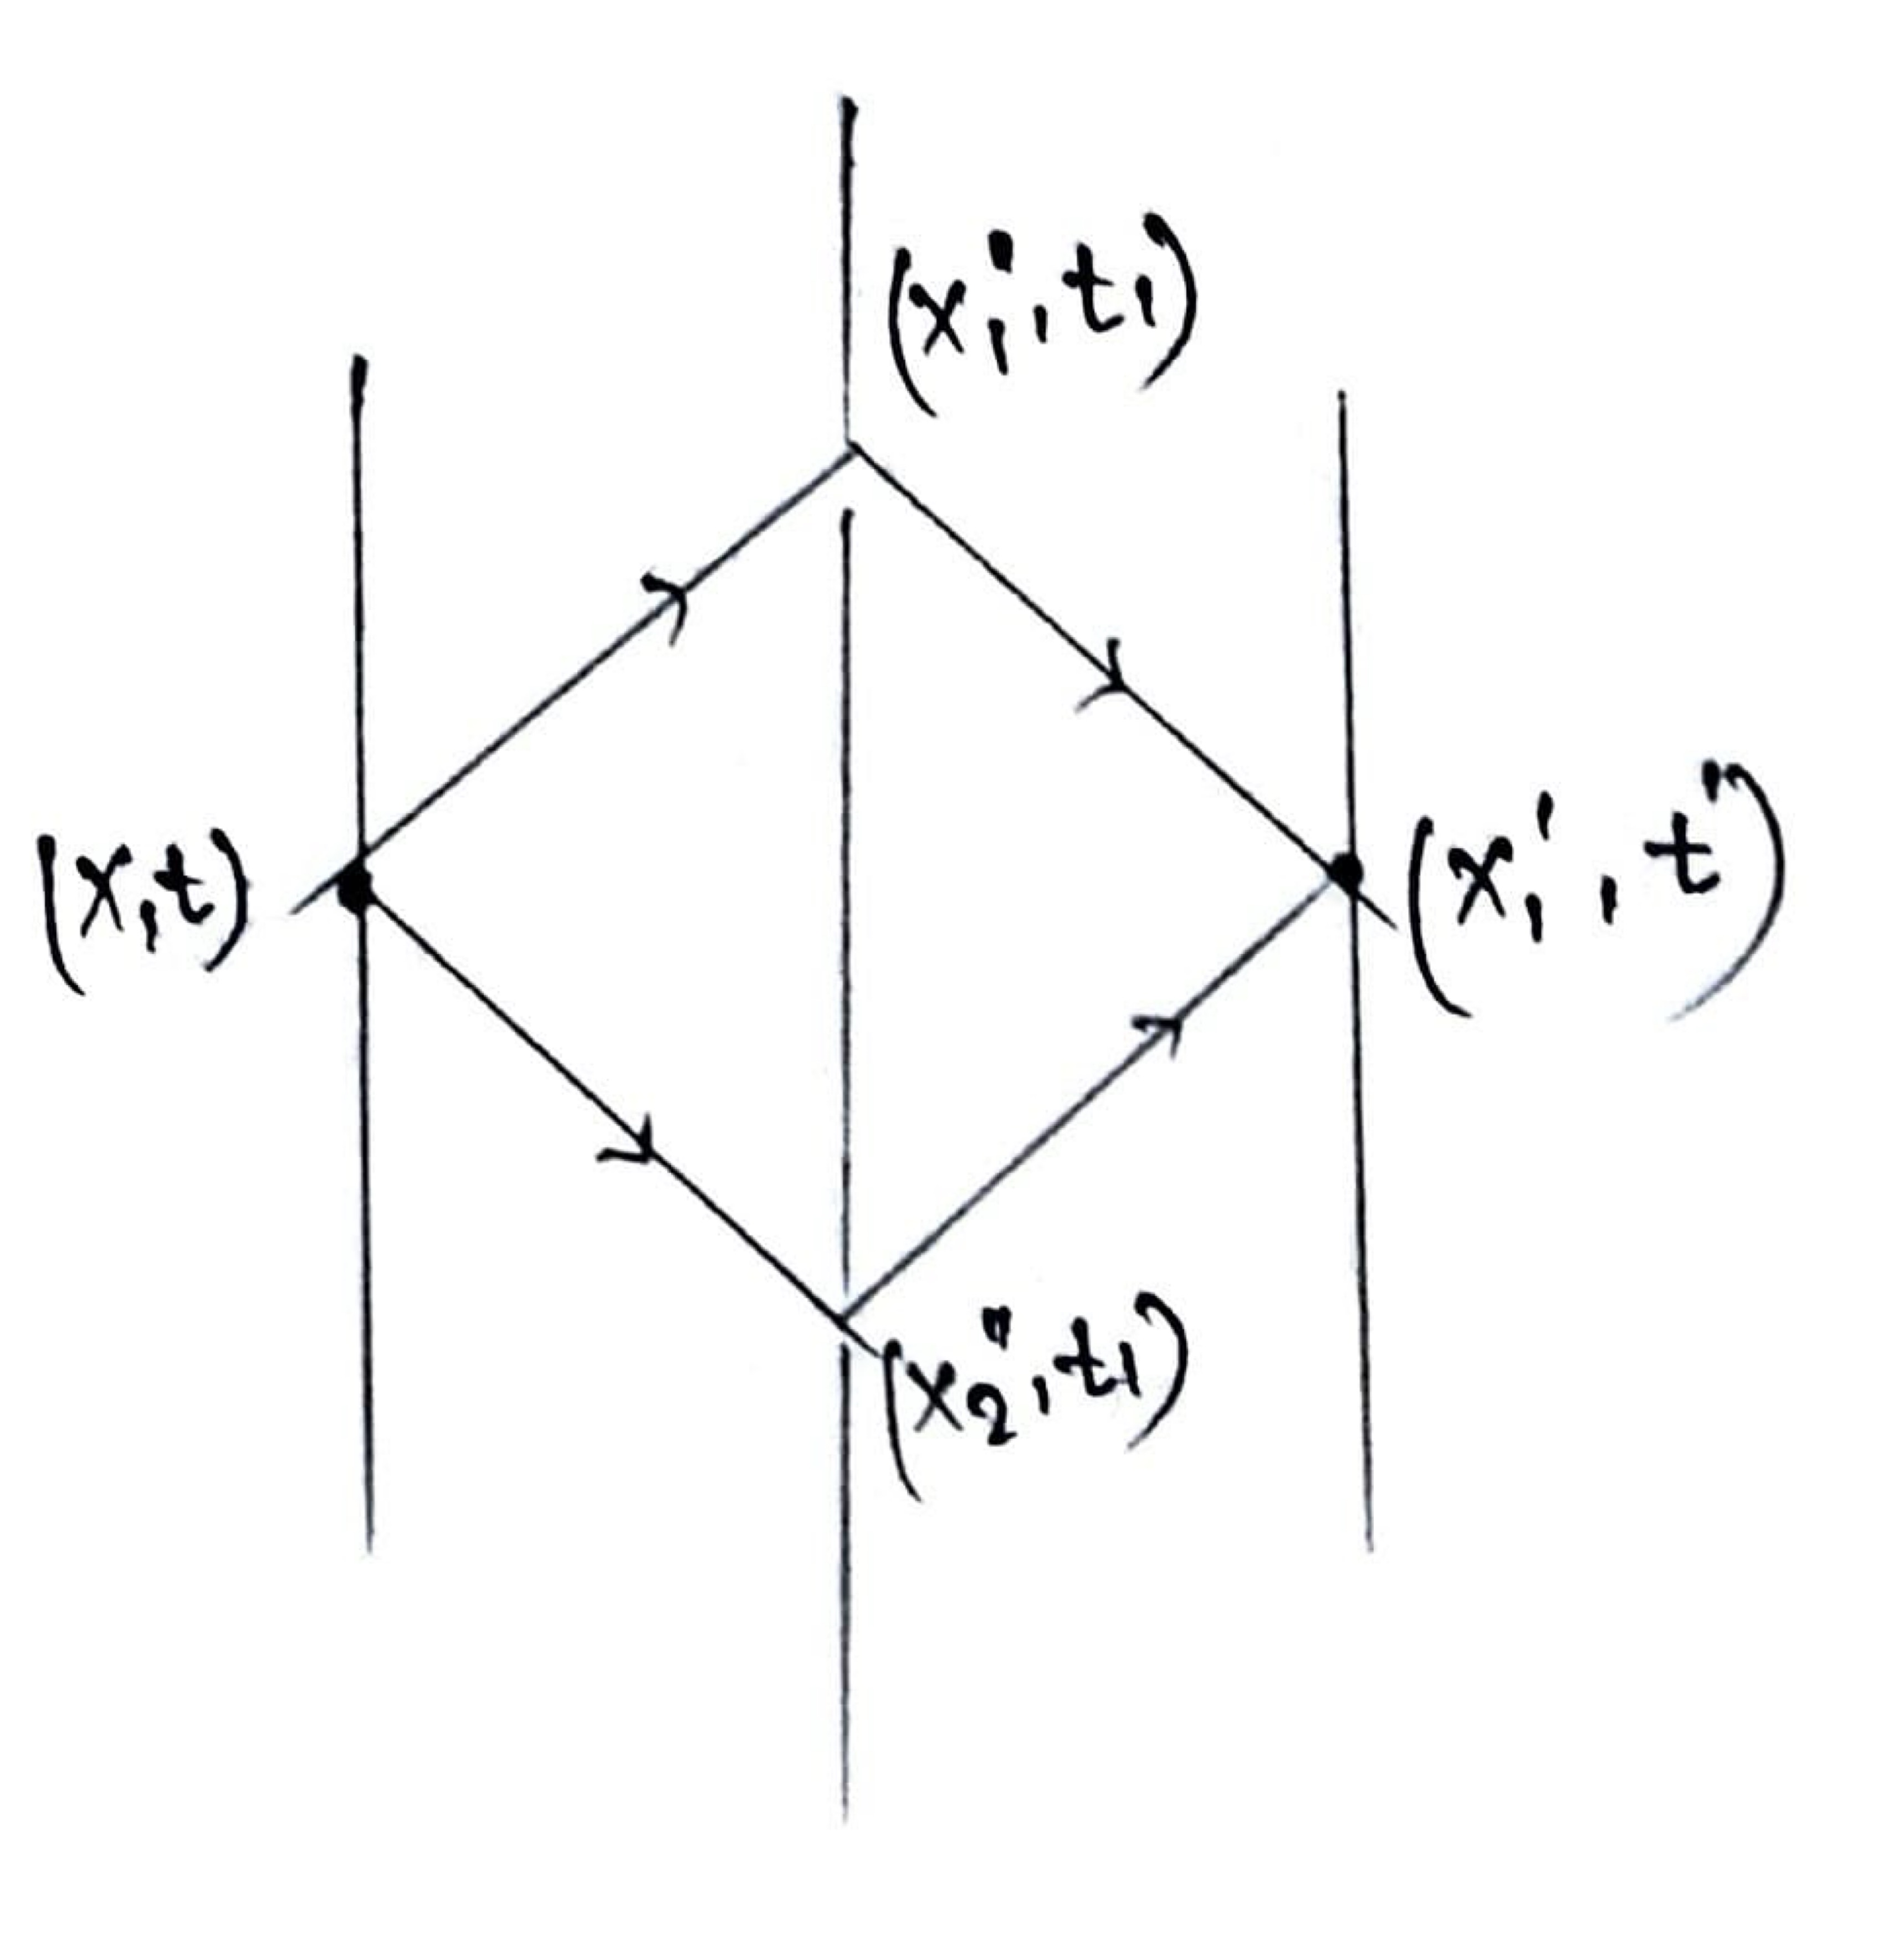
\includegraphics[width=0.5\linewidth]{figures/C10_4.jpeg}
    \caption*{}
\end{figure}
\vspace{-2cm}
\begin{align*}
\langle x', t' | x, t \rangle &= \sum_i \langle x', t' | x_i'', t_2 \rangle \langle x_i'', t_2 | x, t \rangle
 \\
&= \int dx'' \, \langle x', t' | x'' \rangle \langle x' | t \rangle
\end{align*}
\textbf{Completeness Theorem:}
\[
\int dx'' \, \ket{x''} \bra{x''} = \mathbb{I} \quad \to \quad \text{must be a complete set.}
\]
All calculations hereafter are to be done on a discrete space-time and we will take the continuum limit.\\

\noindent
Hence,
\[
\langle x', t' | x, t \rangle = \int \prod_{i=1}^N dx_i \, \langle x', t' | x_{i-1} \rangle \langle x_{i-1}| x_{i-2} \rangle \langle x_{i-2}| \dots \rangle \langle x_1 | x, t \rangle
\]
Now, we need to measure:
\[
\langle x',\, t + \delta t \,| x, t \rangle
\]
Recall,
\[
\langle x, t | \psi \rangle_H = \langle x | \psi, t \rangle_S
\]
Schrödinger equation:
\begin{align*}
i \frac{\partial}{\partial t} \ket{\psi(t)} &= \hat{H} \ket{\psi} \\
\Rightarrow \ket{\psi(t)} &= e^{-i \hat{H} t}  \ket{\psi(0)} = e^{- i \hat{H}t } |\psi \rangle_H \\
\therefore  \langle x | \psi, t \rangle_S &= \langle x | e^{-i \hat{H} t} \ket{\psi}_H
\end{align*}
\[
\boxed{\therefore \langle x',\, t + dt | x, t \rangle 
= \langle x', \Delta t | x,0 \rangle =  ~_H\langle x' | e^{-i \hat{H} t} | x \rangle_H}
\]
\[
\big[ \text{ here, } ~_H\langle x' | e^{-i \hat{H} t} | x \rangle_H \to \text{measure at the same time} \big]
\]
Note as $\Delta t \to 0$,
\[
\langle x', \Delta t | x,0 \rangle = \delta(x - x') \quad \text{(compare at the same time)}
\]
Hence,
\begin{align*}
\langle x' | e^{-i \hat{H} \Delta t} | x \rangle &= \int dp \, \langle x' | e^{-i \hat{H} \Delta t} |p \rangle \langle p | x \rangle \\
&= \int dp \, dp' \, \langle x' | p' \rangle \langle p' | e^{-i \hat{H} \Delta t} | p \rangle \langle p | x \rangle \\
&= \int dp \, dp' \, \frac{1}{2\pi} e^{ip'x'} \langle p' | e^{-i \hat{H} \Delta t} | p \rangle ~e^{-ipx} \\
&\quad \quad \big[ \because \langle x|p \rangle = \frac{1}{\sqrt{2 \pi}} e^{ipx} ; \hbar=1 \big] \\
&= \frac{1}{2\pi}\int dp \, dp' \,  e^{i(p'x'-px)}\, \langle p' | e^{-i \hat{H} \Delta t} | p \rangle \\
\end{align*}
Now, for a free particle,
\[
\hat{H} = \frac{\hat{p}^2}{2m} \quad \big[ V(x) ~\text{not discussed here} \big]
\]
Hence,
\begin{align*}
\langle p' | e^{-i \hat{H} \Delta t} | p \rangle &= \langle p' | e^{-i \frac{\hat{p}^2}{2m} \Delta t} | p \rangle\\
&= e^{-i \frac{\hat{p}^2}{2m}} \langle p'|p \rangle \\
&= e^{-i \frac{p^2}{2m} \Delta t} \delta(p - p')
\end{align*}
Therefore,
\begin{align*}
\langle x' | e^{-i \hat{H} \Delta t} | x \rangle &= \frac{1}{2\pi} \int dp \, dp' \, e^{i(p' x' - p x)} e^{-i \frac{p^2}{2m} \Delta t} \delta(p - p') \\
&= \frac{1}{2\pi} \int dp \, e^{i (p x' - px)} e^{-i \frac{p^2}{2m} \Delta t}
\end{align*}
Using the Gaussian integral identity:
\[
\int_{-\infty}^{\infty} dz \, e^{-a z^2 + b z} = \sqrt{\frac{\pi}{a}} e^{\frac{b^2}{4a}}
\]
We get,
\begin{align*}
&= \frac{1}{2\pi} \int dp \,e^{- {(\frac{i \Delta t}{2m})}^2 p^2} ~ e^{ ip [ x' -x ] } \\
&= \frac{1}{2\pi} \left( \frac{\pi}{\frac{i \Delta t}{2m}} \right)^{1/2} 
e^{- \frac{(x' - x)^2}{4 i \Delta t / (2m)}} \\
&= \left( \frac{m}{2 \pi i \Delta t} \right)^{1/2} 
e^{i \frac{m}{2} {\left( \frac{x' - x}{\Delta t} \right)}^2 \Delta t} \\
&= \left( \frac{m}{2 \pi i \Delta t} \right)^{1/2} 
e^{i \frac{m}{2} v^2 \Delta t} \\\\
&= A ~ e^{ i \mathcal{L} \Delta t } \quad ; \quad \big[ A= \left( \frac{m}{2 \pi i \Delta t} \right)^{1/2} \big] \quad
\end{align*}
So,
\[
\langle x', t' | x, t \rangle = \int dx'\,dx'' \, \prod_i e^{{i m \big[\frac{x_{i+1} - x_i}{2 \Delta t}}\big]^2} = \int \mathcal{D}x \, e^{i S[x]}
\]
Where $\mathcal{D}x$ is an infinite-dimensional factor.




%-------------------------------
% Document ends
%-------------------------------
\end{document}
